\documentclass[]{book}
\usepackage{lmodern}
\usepackage{amssymb,amsmath}
\usepackage{ifxetex,ifluatex}
\usepackage{fixltx2e} % provides \textsubscript
\ifnum 0\ifxetex 1\fi\ifluatex 1\fi=0 % if pdftex
  \usepackage[T1]{fontenc}
  \usepackage[utf8]{inputenc}
\else % if luatex or xelatex
  \ifxetex
    \usepackage{mathspec}
  \else
    \usepackage{fontspec}
  \fi
  \defaultfontfeatures{Ligatures=TeX,Scale=MatchLowercase}
\fi
% use upquote if available, for straight quotes in verbatim environments
\IfFileExists{upquote.sty}{\usepackage{upquote}}{}
% use microtype if available
\IfFileExists{microtype.sty}{%
\usepackage[]{microtype}
\UseMicrotypeSet[protrusion]{basicmath} % disable protrusion for tt fonts
}{}
\PassOptionsToPackage{hyphens}{url} % url is loaded by hyperref
\usepackage[unicode=true]{hyperref}
\hypersetup{
            pdftitle={WildCo: Examples of camera trap data exploration and analysis in R},
            pdfauthor={WildCo Lab, UBC},
            pdfborder={0 0 0},
            breaklinks=true}
\urlstyle{same}  % don't use monospace font for urls
\usepackage{natbib}
\bibliographystyle{apalike}
\usepackage{color}
\usepackage{fancyvrb}
\newcommand{\VerbBar}{|}
\newcommand{\VERB}{\Verb[commandchars=\\\{\}]}
\DefineVerbatimEnvironment{Highlighting}{Verbatim}{commandchars=\\\{\}}
% Add ',fontsize=\small' for more characters per line
\usepackage{framed}
\definecolor{shadecolor}{RGB}{248,248,248}
\newenvironment{Shaded}{\begin{snugshade}}{\end{snugshade}}
\newcommand{\KeywordTok}[1]{\textcolor[rgb]{0.13,0.29,0.53}{\textbf{#1}}}
\newcommand{\DataTypeTok}[1]{\textcolor[rgb]{0.13,0.29,0.53}{#1}}
\newcommand{\DecValTok}[1]{\textcolor[rgb]{0.00,0.00,0.81}{#1}}
\newcommand{\BaseNTok}[1]{\textcolor[rgb]{0.00,0.00,0.81}{#1}}
\newcommand{\FloatTok}[1]{\textcolor[rgb]{0.00,0.00,0.81}{#1}}
\newcommand{\ConstantTok}[1]{\textcolor[rgb]{0.00,0.00,0.00}{#1}}
\newcommand{\CharTok}[1]{\textcolor[rgb]{0.31,0.60,0.02}{#1}}
\newcommand{\SpecialCharTok}[1]{\textcolor[rgb]{0.00,0.00,0.00}{#1}}
\newcommand{\StringTok}[1]{\textcolor[rgb]{0.31,0.60,0.02}{#1}}
\newcommand{\VerbatimStringTok}[1]{\textcolor[rgb]{0.31,0.60,0.02}{#1}}
\newcommand{\SpecialStringTok}[1]{\textcolor[rgb]{0.31,0.60,0.02}{#1}}
\newcommand{\ImportTok}[1]{#1}
\newcommand{\CommentTok}[1]{\textcolor[rgb]{0.56,0.35,0.01}{\textit{#1}}}
\newcommand{\DocumentationTok}[1]{\textcolor[rgb]{0.56,0.35,0.01}{\textbf{\textit{#1}}}}
\newcommand{\AnnotationTok}[1]{\textcolor[rgb]{0.56,0.35,0.01}{\textbf{\textit{#1}}}}
\newcommand{\CommentVarTok}[1]{\textcolor[rgb]{0.56,0.35,0.01}{\textbf{\textit{#1}}}}
\newcommand{\OtherTok}[1]{\textcolor[rgb]{0.56,0.35,0.01}{#1}}
\newcommand{\FunctionTok}[1]{\textcolor[rgb]{0.00,0.00,0.00}{#1}}
\newcommand{\VariableTok}[1]{\textcolor[rgb]{0.00,0.00,0.00}{#1}}
\newcommand{\ControlFlowTok}[1]{\textcolor[rgb]{0.13,0.29,0.53}{\textbf{#1}}}
\newcommand{\OperatorTok}[1]{\textcolor[rgb]{0.81,0.36,0.00}{\textbf{#1}}}
\newcommand{\BuiltInTok}[1]{#1}
\newcommand{\ExtensionTok}[1]{#1}
\newcommand{\PreprocessorTok}[1]{\textcolor[rgb]{0.56,0.35,0.01}{\textit{#1}}}
\newcommand{\AttributeTok}[1]{\textcolor[rgb]{0.77,0.63,0.00}{#1}}
\newcommand{\RegionMarkerTok}[1]{#1}
\newcommand{\InformationTok}[1]{\textcolor[rgb]{0.56,0.35,0.01}{\textbf{\textit{#1}}}}
\newcommand{\WarningTok}[1]{\textcolor[rgb]{0.56,0.35,0.01}{\textbf{\textit{#1}}}}
\newcommand{\AlertTok}[1]{\textcolor[rgb]{0.94,0.16,0.16}{#1}}
\newcommand{\ErrorTok}[1]{\textcolor[rgb]{0.64,0.00,0.00}{\textbf{#1}}}
\newcommand{\NormalTok}[1]{#1}
\usepackage{longtable,booktabs}
% Fix footnotes in tables (requires footnote package)
\IfFileExists{footnote.sty}{\usepackage{footnote}\makesavenoteenv{long table}}{}
\usepackage{graphicx,grffile}
\makeatletter
\def\maxwidth{\ifdim\Gin@nat@width>\linewidth\linewidth\else\Gin@nat@width\fi}
\def\maxheight{\ifdim\Gin@nat@height>\textheight\textheight\else\Gin@nat@height\fi}
\makeatother
% Scale images if necessary, so that they will not overflow the page
% margins by default, and it is still possible to overwrite the defaults
% using explicit options in \includegraphics[width, height, ...]{}
\setkeys{Gin}{width=\maxwidth,height=\maxheight,keepaspectratio}
\IfFileExists{parskip.sty}{%
\usepackage{parskip}
}{% else
\setlength{\parindent}{0pt}
\setlength{\parskip}{6pt plus 2pt minus 1pt}
}
\setlength{\emergencystretch}{3em}  % prevent overfull lines
\providecommand{\tightlist}{%
  \setlength{\itemsep}{0pt}\setlength{\parskip}{0pt}}
\setcounter{secnumdepth}{5}
% Redefines (sub)paragraphs to behave more like sections
\ifx\paragraph\undefined\else
\let\oldparagraph\paragraph
\renewcommand{\paragraph}[1]{\oldparagraph{#1}\mbox{}}
\fi
\ifx\subparagraph\undefined\else
\let\oldsubparagraph\subparagraph
\renewcommand{\subparagraph}[1]{\oldsubparagraph{#1}\mbox{}}
\fi

% set default figure placement to htbp
\makeatletter
\def\fps@figure{htbp}
\makeatother

\usepackage{booktabs}
\usepackage{amsthm}
\makeatletter
\def\thm@space@setup{%
  \thm@preskip=8pt plus 2pt minus 4pt
  \thm@postskip=\thm@preskip
}
\makeatother
\usepackage{booktabs}
\usepackage{longtable}
\usepackage{array}
\usepackage{multirow}
\usepackage{wrapfig}
\usepackage{float}
\usepackage{colortbl}
\usepackage{pdflscape}
\usepackage{tabu}
\usepackage{threeparttable}
\usepackage{threeparttablex}
\usepackage[normalem]{ulem}
\usepackage{makecell}
\usepackage{xcolor}

\title{WildCo: Examples of camera trap data exploration and analysis in R}
\author{WildCo Lab, UBC}
\date{2021-05-17}

\begin{document}
\maketitle

{
\setcounter{tocdepth}{1}
\tableofcontents
}
\chapter{Introduction}\label{introduction}

\section{What this guide is}\label{what-this-guide-is}

\begin{itemize}
\tightlist
\item
  An R code reference manual for basic concepts in the exploration and
  analysis of camera data
\item
  A tool to provide hands on experience of standardised camera trap data
  in R
\item
  A link to resources and papers which showcase the types of analyses
  you can perform (and would maybe want to replicate in the future)
\item
  A `living' document - it will updated and curated by different lab
  members through time
\end{itemize}

\section{What this guide is not}\label{what-this-guide-is-not}

\begin{itemize}
\tightlist
\item
  The ``best'' way to explore / analyse your data (although we hopefully
  provide a good foundation)
\item
  The ``best'' R code for camera traps
\item
  A static document
\end{itemize}

\section{How to use this handbook}\label{how-to-use-this-handbook}

\begin{itemize}
\tightlist
\item
  Browse the pages in the Table of Contents, or use the search box
\item
  You can follow-along with the example data
\item
  Explore addition ``Resources'' at the end of each section for great
  applications of camera trap data
\end{itemize}

\section{Get in touch}\label{get-in-touch}

If you have any questions about this document and the information it
contains, please \href{wildco.lab@gmail.com}{email us} or better still,
submit an issue on our
\href{https://github.com/WildCoLab/WildCo_Data_Analysis}{data analysis
GitHub page}.

\section{Acknowledgements}\label{acknowledgements}

This guide is produced by the members of the Wildlife Coexistence Lab at
UBC. Check out our \href{}{website}

\chapter{Data standardisation}\label{data-standardisation}

The benefits of `standardizing' our use of camera traps, or other
sensors of biodiversity, are clear: It allows us to rapidly explore and
analyse camera trap data, apply tools created elsewhere, and synthesise
data from different projects. Ultimately resulting in more robust,
repeatable, and timely science and managament decisions.

This is just as true for the process by which we design and implement
our camera trap studies, as it is for how we curate and analyse the
resultant data. That said, it is becoming increasingly clear that we
will \textbf{never} fully standardise camera trap data. Although this is
sounds somewhat defeatist, the number of different data standards which
exist is increasing, and is a reflection of the different requirements
of researchers, practitioners and research aims/objectives of the camera
trapping community.

That doesnt mean we should not standardise our data however! Simply that
we should be clear about the standards we adopt, and stick to them like
glue.

\section{The WildCo Lab data
standard}\label{the-wildco-lab-data-standard}

\chapter{Data Exploration}\label{data-exploration}

The most important part of analysing camera trap data is exploring and
checking your data. All to frequently, we find that researchers do not
have a thorough grasp for the quality of their datasets!

Dynamic exploration is key - do not leave it until the end. Also, plot
from your dataframes.

\begin{Shaded}
\begin{Highlighting}[]
\CommentTok{# ADD THE DATA FRAMES HERE}
\end{Highlighting}
\end{Shaded}

\section{Standardised exploration
script}\label{standardised-exploration-script}

In the Wildlife coexistance lab we use a standardised R script to
generate summary information for camera trap projects. The most up to
date script for exploring a single site can be found on our
\href{https://github.com/WildCoLab/SingleSiteExploration}{GitHub page}.

\subsection{The output}\label{the-output}

\begin{Shaded}
\begin{Highlighting}[]
\NormalTok{## ADD THE MARKDOWN CODE HERE}
\end{Highlighting}
\end{Shaded}

\subsubsection{Algar Project}\label{algar-project}

\subsubsection{Camera locations}\label{camera-locations}

To date there have been camera deployments at 20 unique locations.

\includegraphics{bookdown-demo_files/figure-latex/map-1.pdf}

\subsubsection{Camera activity through
time}\label{camera-activity-through-time}

The 20 stations have resulted in a total of 7013 camera days (mean =
350.6 days per station; min = 139; max = 372).The daily break down of
camera activity is as follows:

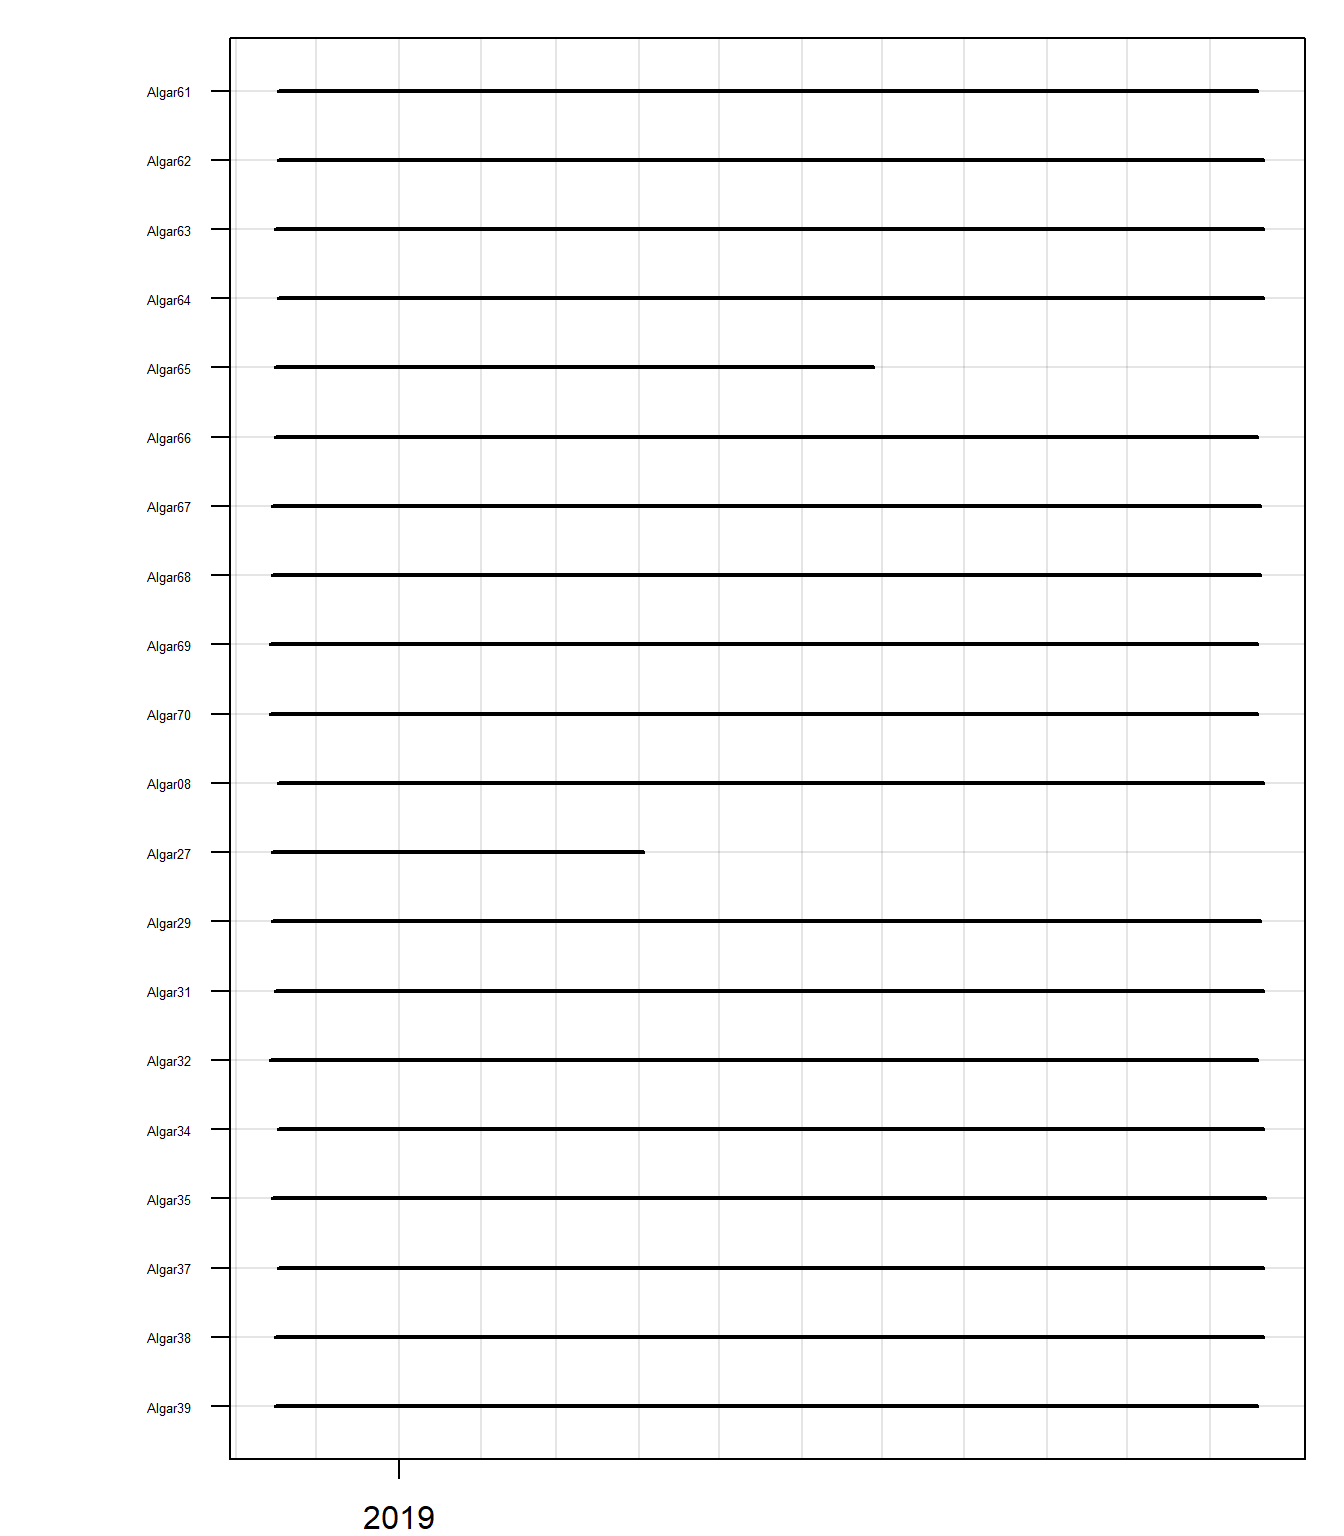
\includegraphics{bookdown-demo_files/figure-latex/activity-1.pdf}

Figure 2: Where black lines denote a camera which is active, white space
indicates cameras which are inactive, grey vertical lines represent the
1st of each calender month.

\subsubsection{Raw camera detections}\label{raw-camera-detections}

To date, there have been 3786 image classifications. Of these, 3786 are
classified as blanks (0\% of the total dataset).

Of the detections which have been identified, there are 12 different
catageories.

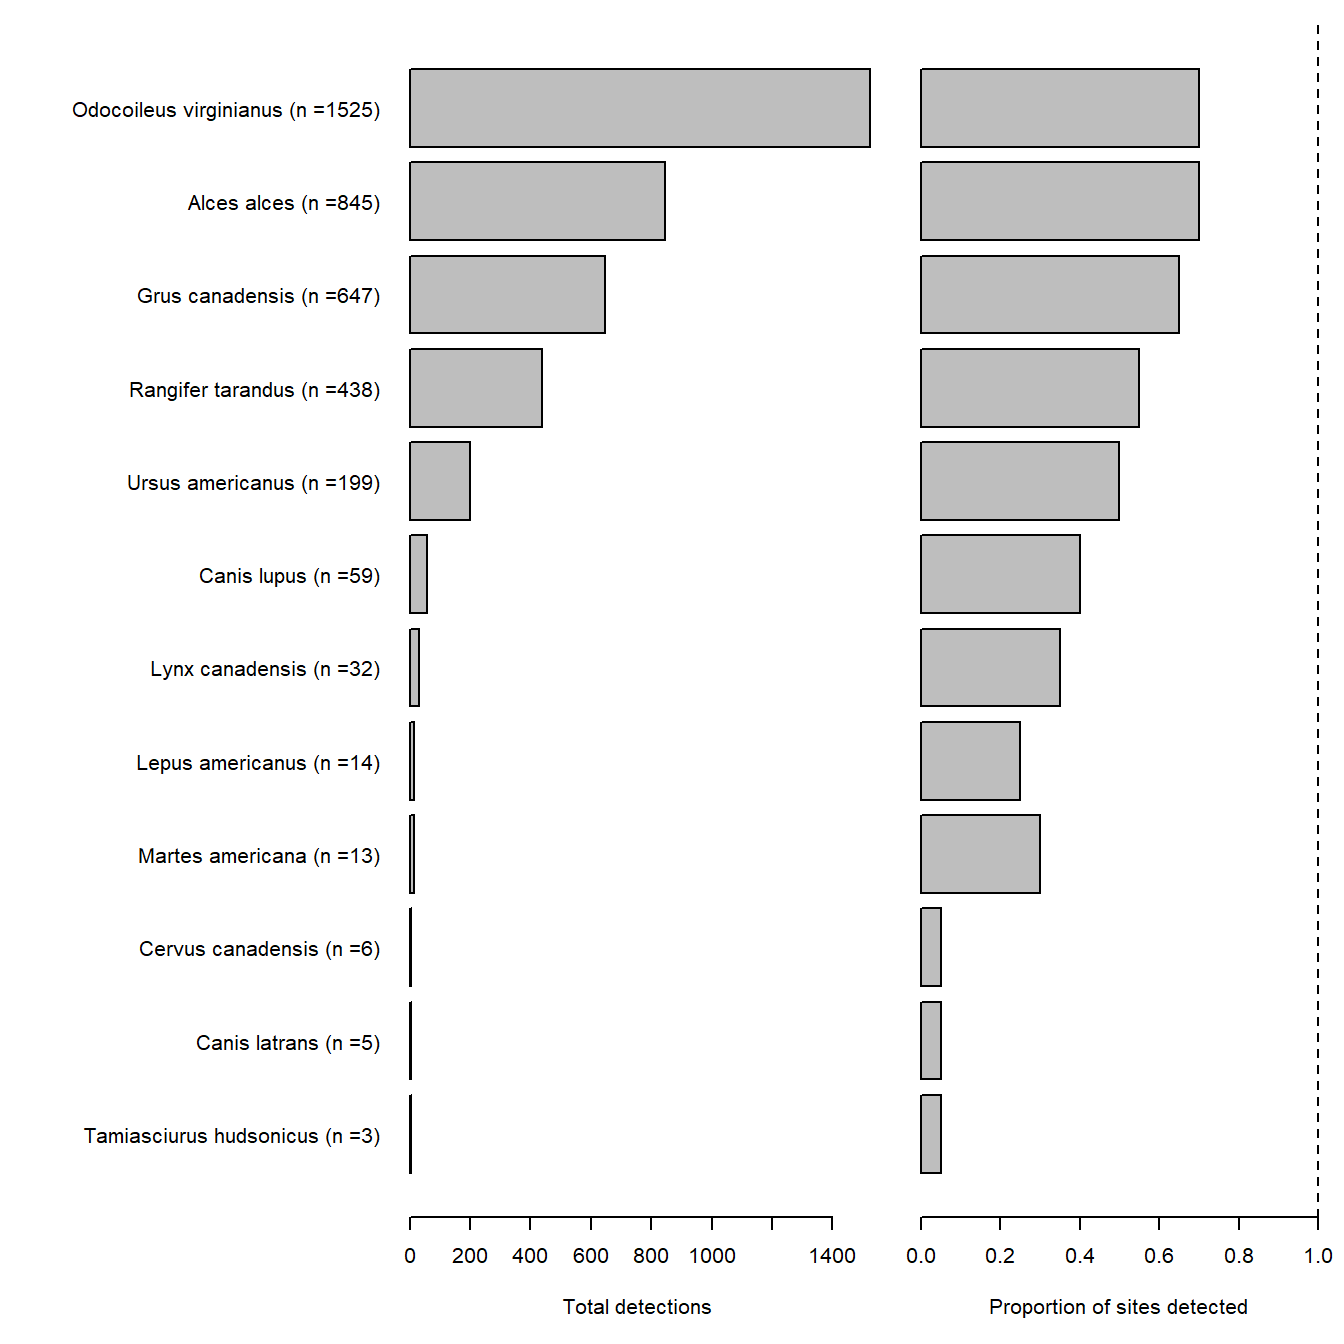
\includegraphics{bookdown-demo_files/figure-latex/captures-1.pdf}

\subsubsection{Detection check}\label{detection-check}

The following plot helps you determine if you have detections occuring
outside of the times cameras are active. \emph{Important note} You can
still get detections outside of the activity period if you have decided
that the field of view was shifted and the data is un-compariable to
that which was collected earlier.

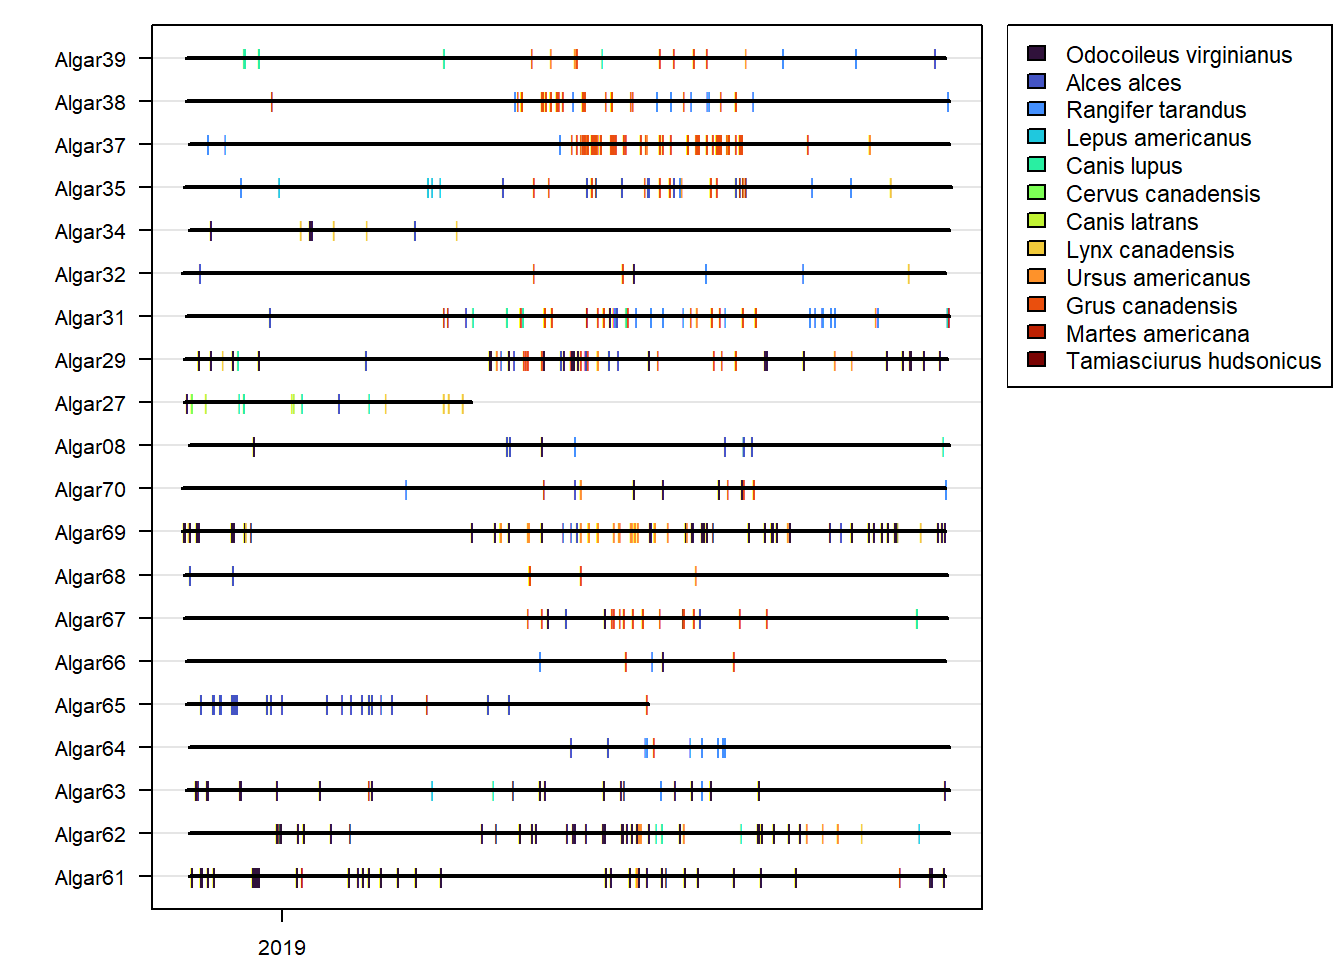
\includegraphics{bookdown-demo_files/figure-latex/detecion summary-1.pdf}

\subsubsection{Species metadata}\label{species-metadata}

Of the images classfied as containing animals, the proportion of
photographs assigned to the following catagories are as follows:

\subsubsection{Sex}\label{sex}

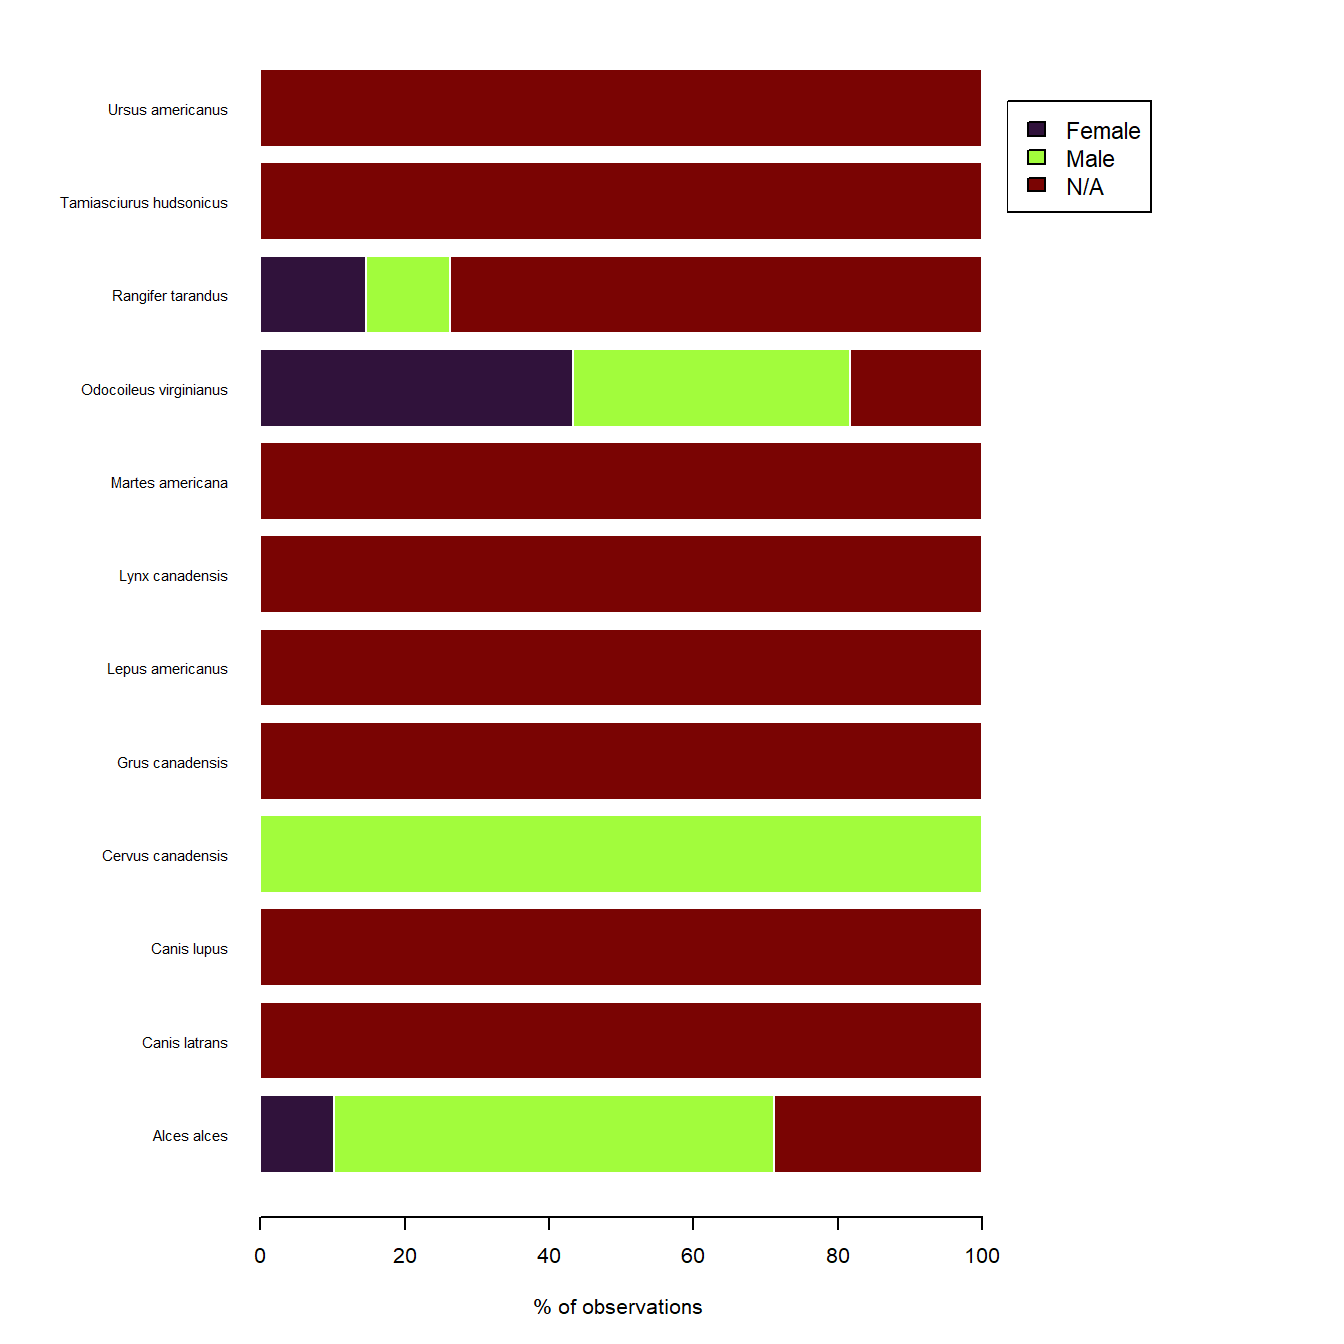
\includegraphics{bookdown-demo_files/figure-latex/sex plot-1.pdf}

\subsubsection{Age}\label{age}

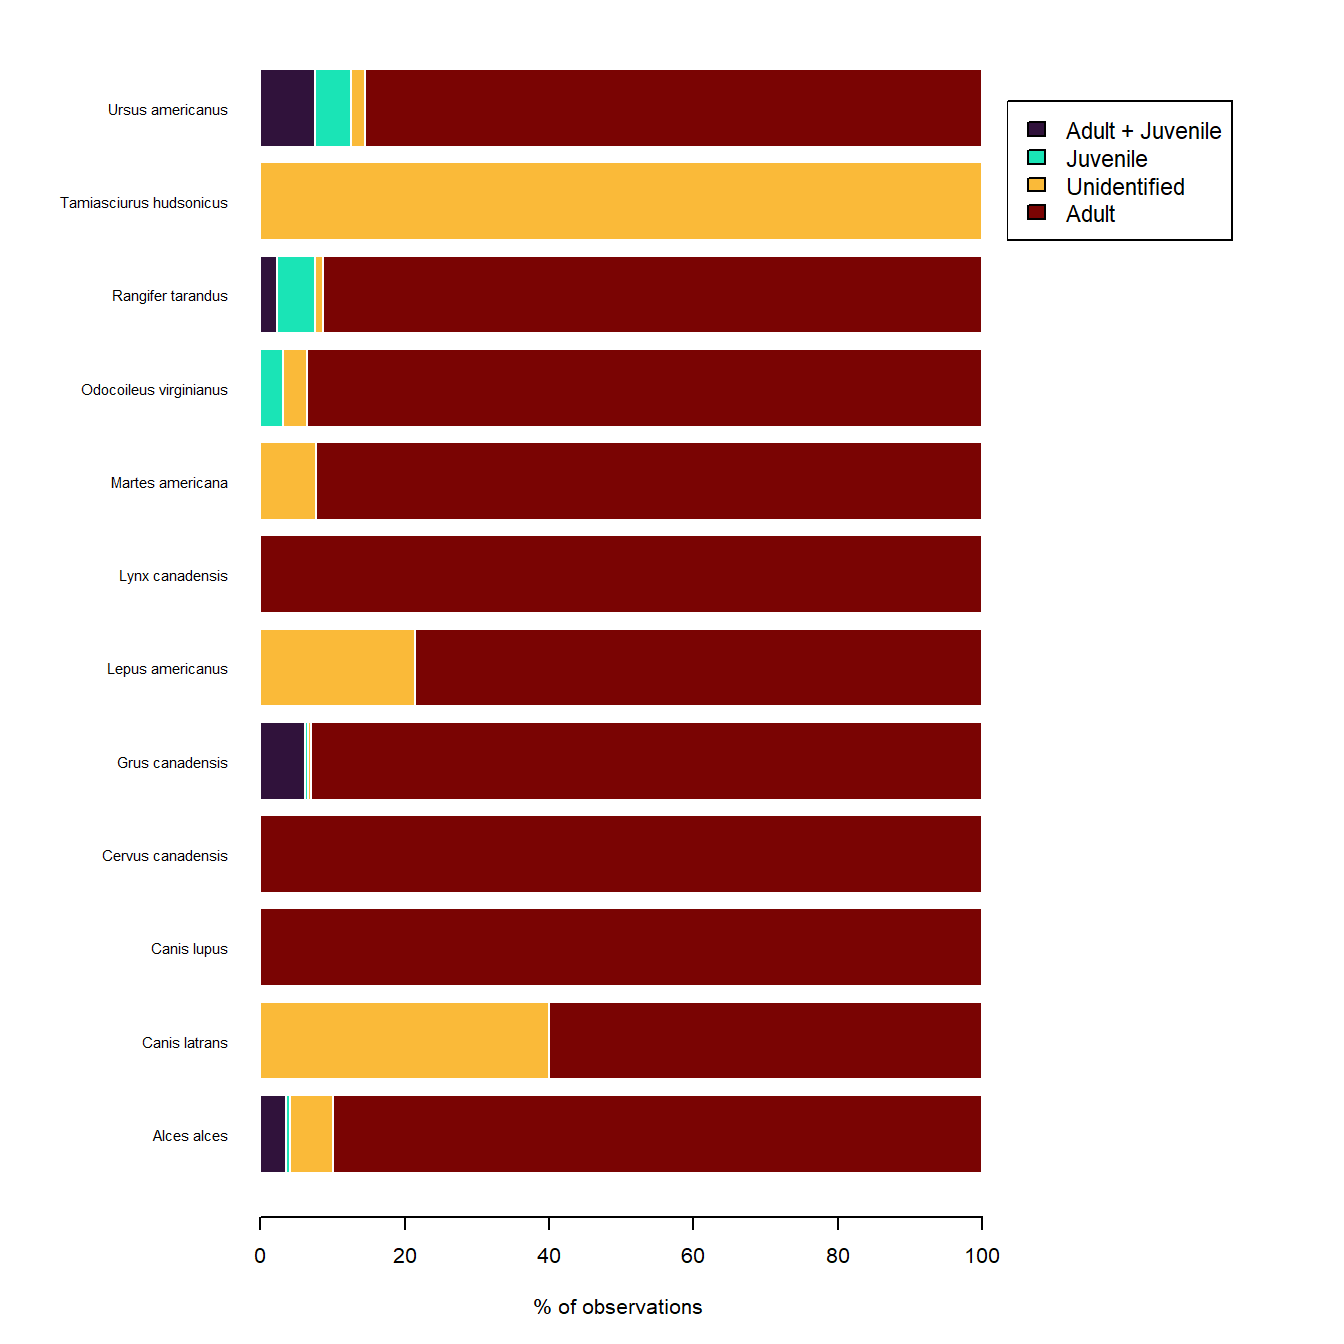
\includegraphics{bookdown-demo_files/figure-latex/age plot-1.pdf}

\subsubsection{Behaviour}\label{behaviour}

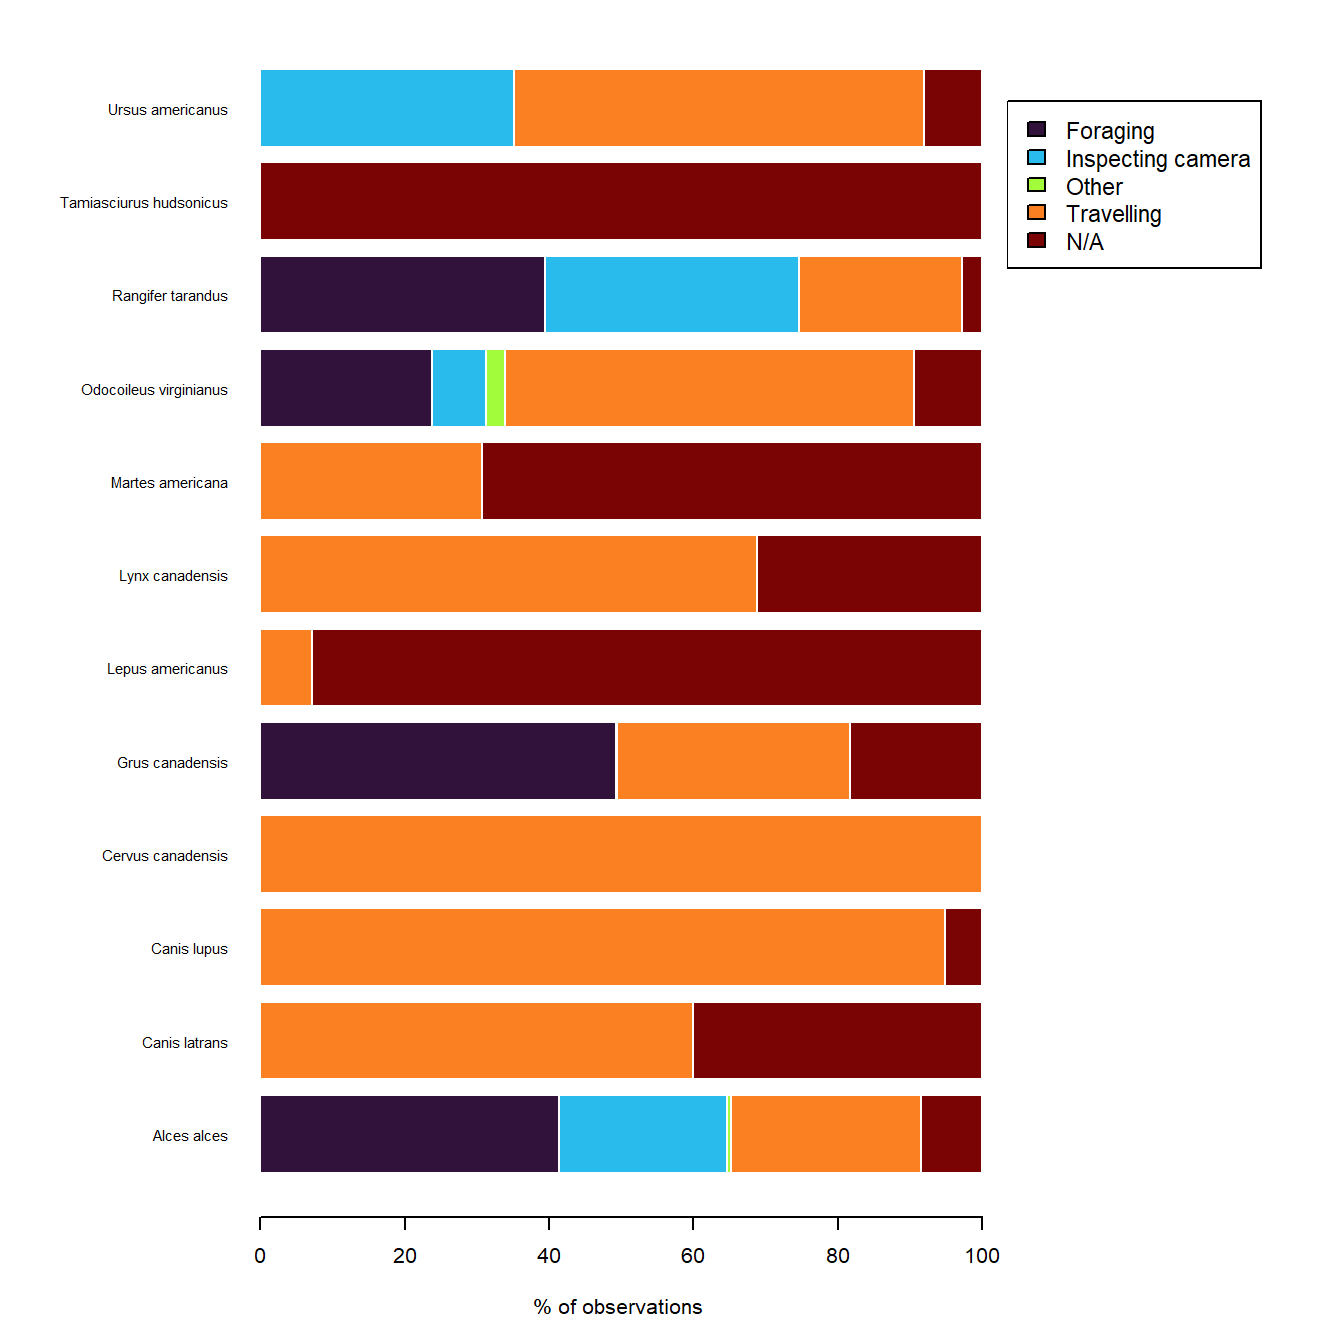
\includegraphics{bookdown-demo_files/figure-latex/behaviour plot-1.pdf}

\subsubsection{Independent camera
detections}\label{independent-camera-detections}

Using an independance threshold of 30 minutes, the number of detections
is reduced to 539. The rest of the analyses are conducted with this
data. The summary of detections is as follows:

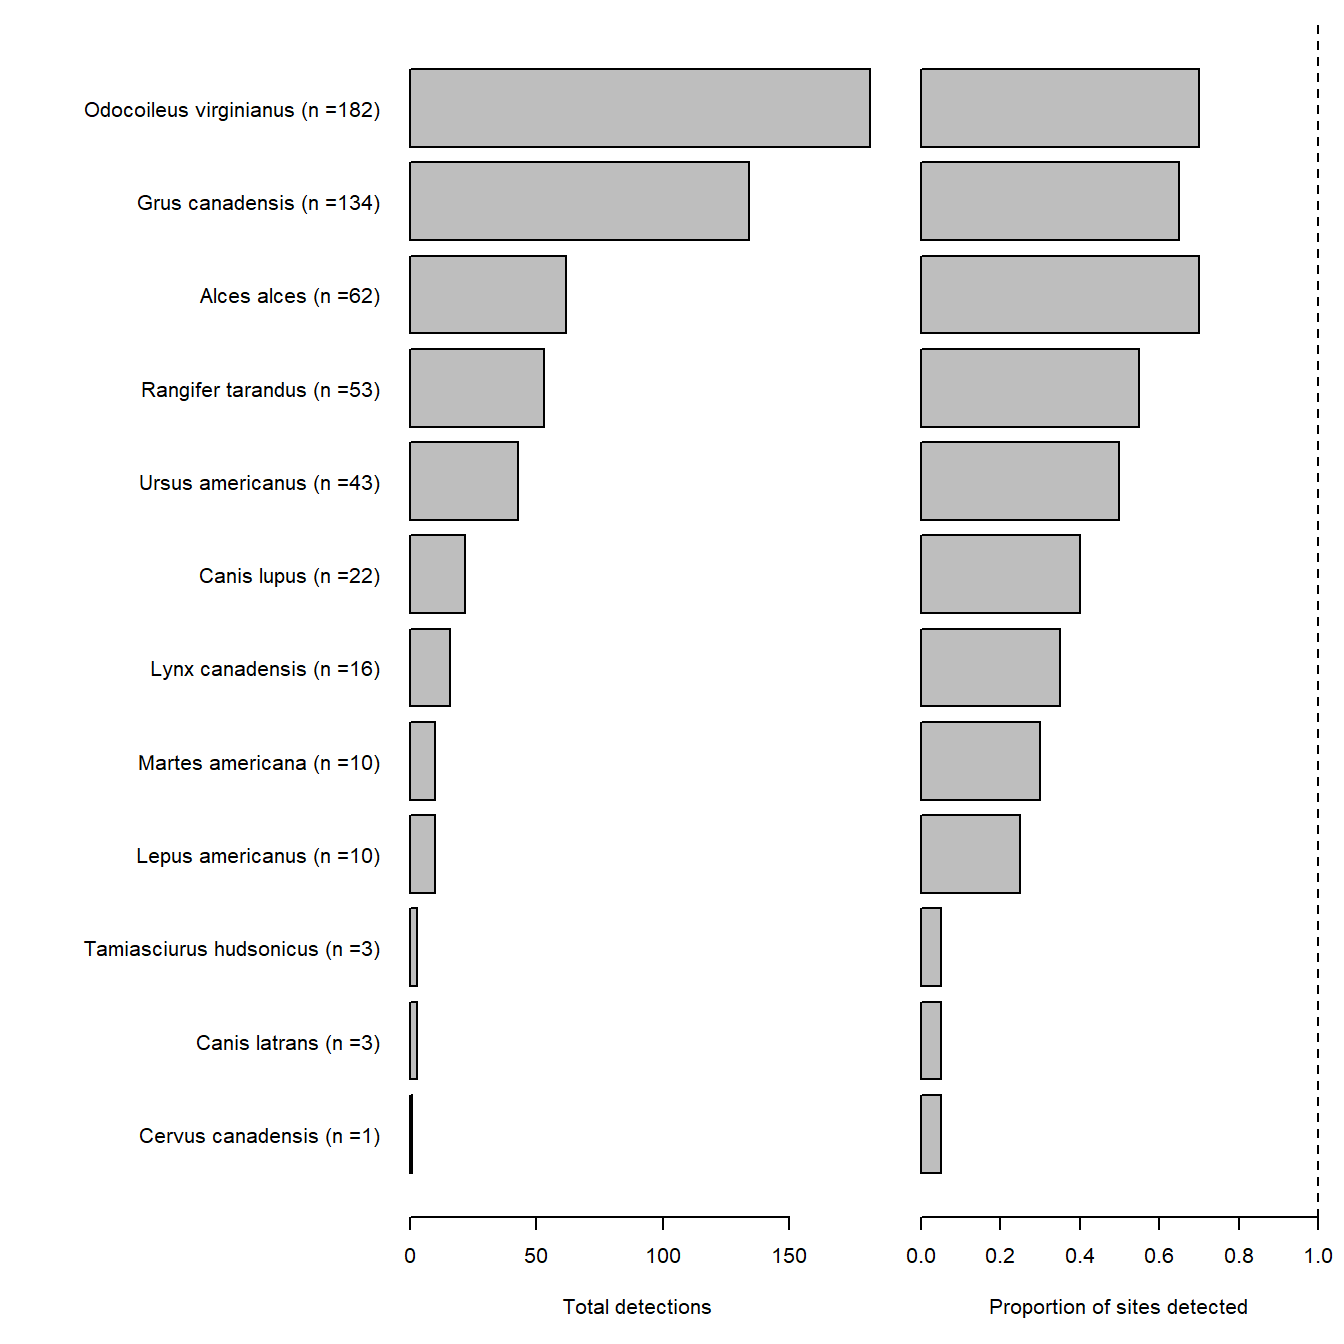
\includegraphics{bookdown-demo_files/figure-latex/ind captures-1.pdf}

\subsubsection{Group size distribution}\label{group-size-distribution}

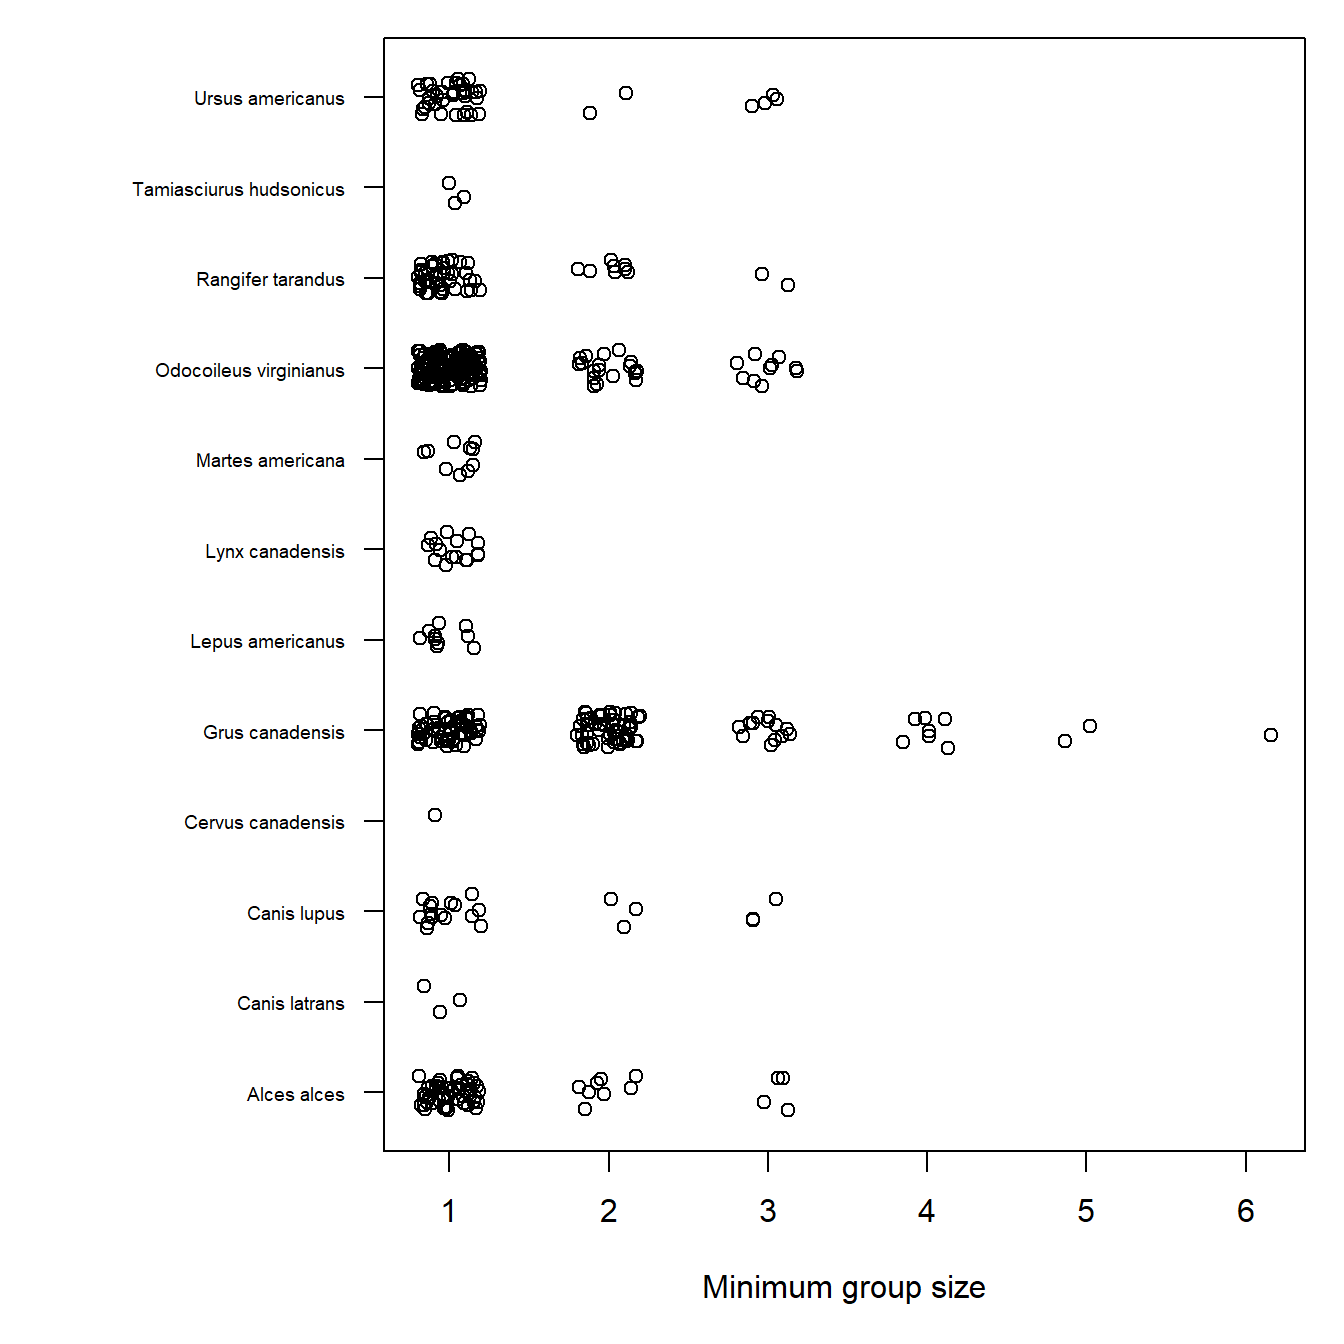
\includegraphics{bookdown-demo_files/figure-latex/group size-1.pdf}

\subsubsection{Site-level species
covariance}\label{site-level-species-covariance}

This plot shows the covariance between different species at the site
level for species with \textgreater{}5 unique detections. For example,
if you typically get lots of caribou and bears at the same site, they
will have positive covariance. If you get caribou where you dont get
bears, they will have negative covariance.

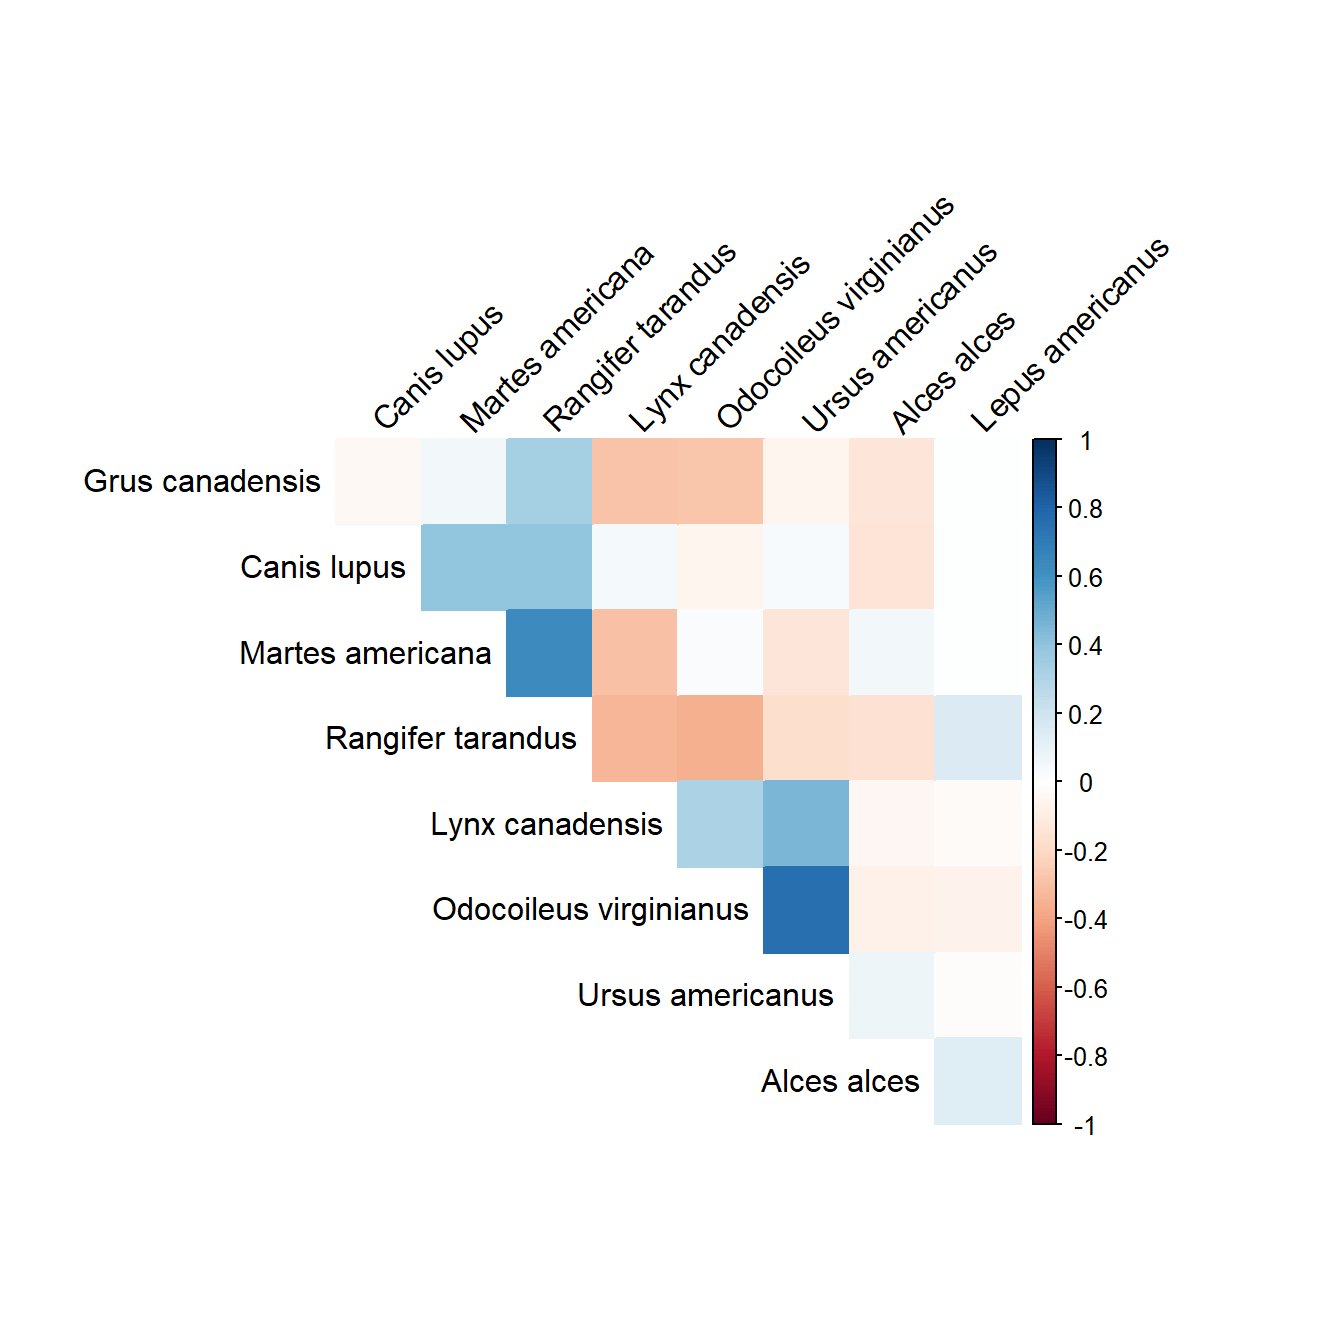
\includegraphics{bookdown-demo_files/figure-latex/covariance-1.pdf}

\subsubsection{Calculate relative
abundance}\label{calculate-relative-abundance}

Note, when calculating relative abundance, we use the minimum group size
column.

\subsubsection{Site-level temporal
plots}\label{site-level-temporal-plots}

\subsubsection{Summary}\label{summary}

Across all sites and species:

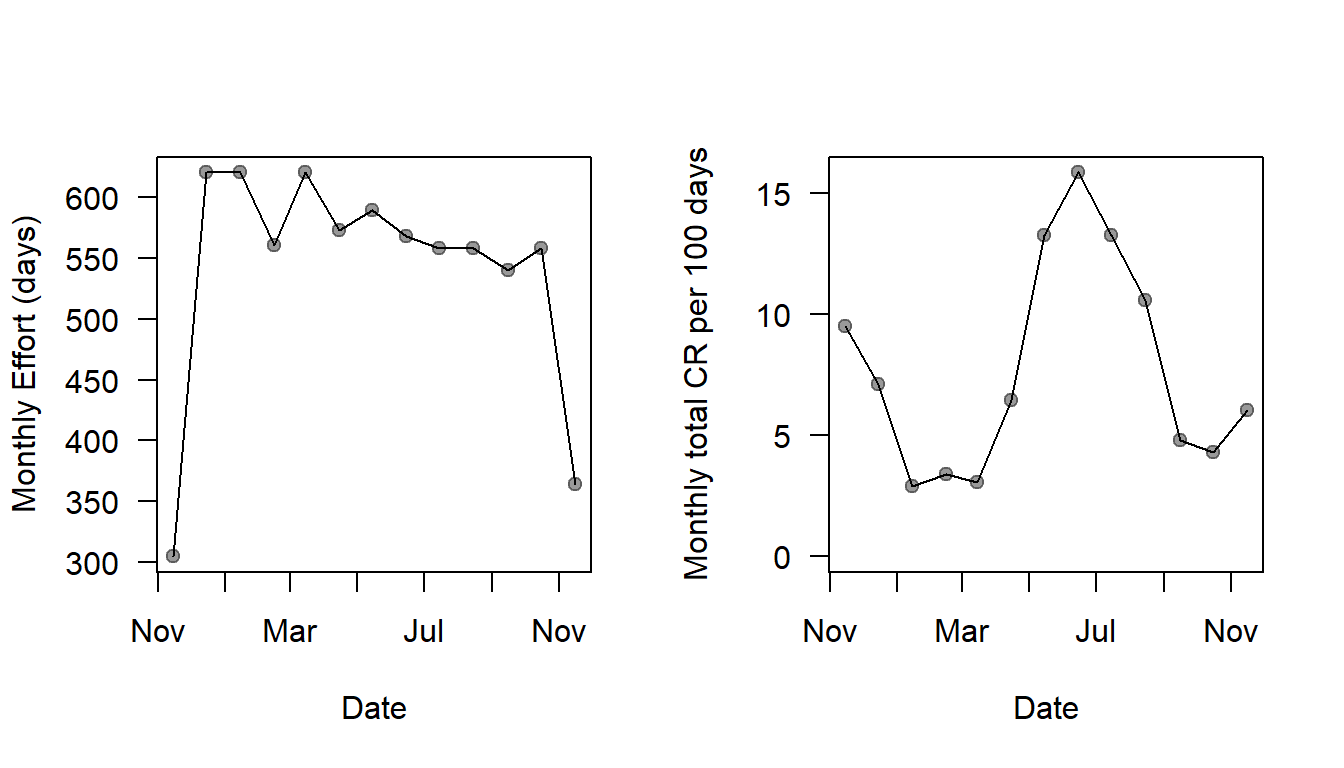
\includegraphics{bookdown-demo_files/figure-latex/overall CR-1.pdf}

\subsubsection{Species-specific temporal
trends}\label{species-specific-temporal-trends}

Species level variation in monthly capture rates are as follows:

\includegraphics{bookdown-demo_files/figure-latex/unnamed-chunk-5-1.pdf}
\includegraphics{bookdown-demo_files/figure-latex/unnamed-chunk-5-2.pdf}

\subsubsection{Data exporting}\label{data-exporting}

This script outputs 9 useful dataframes for future data analysis:

\begin{enumerate}
\def\labelenumi{\arabic{enumi}.}
\tightlist
\item
  A data frame of ``independent detections'' at the 30 minute threshold
  you specified at the start:
\end{enumerate}

\begin{itemize}
\tightlist
\item
  ``data/processed\_data/Algar\_30min\_Independent.csv''
\end{itemize}

2/3: A `site x species' matrix of the number of independent detections
and species counts accross the full study period:

\begin{itemize}
\item
  ``data/processed\_data/Algar\_30min\_Independent\_total\_observations.csv''
\item
  ``data/processed\_data/Algar\_30min\_Independent\_total\_counts.csv''
\end{itemize}

4/5: A `site\_month x species' matrix of the number of independent
detections and species counts accross for each month in the study
period:

\begin{itemize}
\item
  ``data/processed\_data/Algar\_30min\_Monthly\_total\_observations.csv''
\item
  ``data/processed\_data/Algar\_30min\_Monthly\_total\_counts.csv''
\end{itemize}

6/7: A `site\_week x species' matrix of the number of independent
detections and species counts accross for each week in the study period:

\begin{itemize}
\item
  ``data/processed\_data/Algar\_30min\_Weekly\_total\_observations.csv''
\item
  ``data/processed\_data/Algar\_30min\_Weekly\_total\_counts.csv''
\end{itemize}

8/9: A `site\_day x species' matrix of the number of independent
detections and species counts accross for each day a station was active
in the study period:

\begin{itemize}
\item
  ``data/processed\_data/Algar\_30min\_Daily\_total\_observations.csv''
\item
  ``data/processed\_data/Algar\_30min\_Daily\_total\_counts.csv''
\end{itemize}

\subsubsection{Final check}\label{final-check}

If the code is working properly the total observations/counts should be
the same at each temporal scale (total/monthly/weekly). Check this using
the following tables.

\subsubsection{Observations}\label{observations}

\begin{tabu} to \linewidth {>{\raggedright}X>{\raggedleft}X>{\raggedleft}X>{\raggedleft}X>{\raggedleft}X>{\raggedleft}X>{\raggedleft}X>{\raggedleft}X>{\raggedleft}X>{\raggedleft}X>{\raggedleft}X>{\raggedleft}X>{\raggedleft}X>{\raggedleft}X}
\hline
Time & Effort & Alces alces & Canis latrans & Canis lupus & Cervus canadensis & Grus canadensis & Lepus americanus & Lynx canadensis & Martes americana & Odocoileus virginianus & Rangifer tarandus & Tamiasciurus hudsonicus & Ursus americanus\\
\hline
\textbf{Total} & 7033 & 62 & 3 & 22 & 1 & 134 & 10 & 16 & 10 & 182 & 53 & 3 & 43\\
\hline
\textbf{Monthly} & 7033 & 62 & 3 & 22 & 1 & 134 & 10 & 16 & 10 & 182 & 53 & 3 & 43\\
\hline
\textbf{Weekly} & 7033 & 62 & 3 & 22 & 1 & 134 & 10 & 16 & 10 & 182 & 53 & 3 & 43\\
\hline
\textbf{Daily} & 7033 & 62 & 3 & 22 & 1 & 134 & 10 & 16 & 10 & 182 & 53 & 3 & 43\\
\hline
\end{tabu}

\subsubsection{Counts}\label{counts}

\begin{tabu} to \linewidth {>{\raggedright}X>{\raggedleft}X>{\raggedleft}X>{\raggedleft}X>{\raggedleft}X>{\raggedleft}X>{\raggedleft}X>{\raggedleft}X>{\raggedleft}X>{\raggedleft}X>{\raggedleft}X>{\raggedleft}X>{\raggedleft}X>{\raggedleft}X}
\hline
Time & Effort & Alces alces & Canis latrans & Canis lupus & Cervus canadensis & Grus canadensis & Lepus americanus & Lynx canadensis & Martes americana & Odocoileus virginianus & Rangifer tarandus & Tamiasciurus hudsonicus & Ursus americanus\\
\hline
\textbf{Total} & 7033 & 81 & 3 & 31 & 1 & 251 & 10 & 16 & 10 & 225 & 65 & 3 & 53\\
\hline
\textbf{Monthly} & 7033 & 81 & 3 & 31 & 1 & 251 & 10 & 16 & 10 & 225 & 65 & 3 & 53\\
\hline
\textbf{Weekly} & 7033 & 81 & 3 & 31 & 1 & 251 & 10 & 16 & 10 & 225 & 65 & 3 & 53\\
\hline
\textbf{Daily} & 7033 & 81 & 3 & 31 & 1 & 251 & 10 & 16 & 10 & 225 & 65 & 3 & 53\\
\hline
\end{tabu}

\chapter{Common analysis data
formats}\label{common-analysis-data-formats}

When working with standardized datasets, there are three key dataframes
we want to end up with.

\chapter{Community composition}\label{community-composition}

One of the most fundamental questions researchers and practitioners want
to answer with camera traps is \emph{how many species are there?}

To illustrate this, we will continue to use our case study from Northern
Alberta:

\begin{Shaded}
\begin{Highlighting}[]
\CommentTok{# Read in the example dataset}
\NormalTok{dat <-}\StringTok{ }\KeywordTok{read.csv}\NormalTok{(}\StringTok{"data/raw_data/Example_detection_data.csv"}\NormalTok{, }\DataTypeTok{header=}\NormalTok{T)}
\NormalTok{eff <-}\StringTok{ }\KeywordTok{read.csv}\NormalTok{(}\StringTok{"data/raw_data/Example_deployment_data.csv"}\NormalTok{, }\DataTypeTok{header=}\NormalTok{T)}
\NormalTok{sta <-}\StringTok{ }\KeywordTok{read.csv}\NormalTok{(}\StringTok{"data/raw_data/Example_station_data.csv"}\NormalTok{, }\DataTypeTok{header=}\NormalTok{T)}
\end{Highlighting}
\end{Shaded}

\section{Observed richness}\label{observed-richness}

The simplest way to quantify species richness is counting the number of
species you detect on your camera traps - `observed richness'. In the
case of the example data set, this represents 12 species.

\begin{table}
\centering
\begin{tabular}[t]{l|r}
\hline
Species\_observed & Species\_count\\
\hline
Odocoileus virginianus & 1\\
\hline
Alces alces & 2\\
\hline
Rangifer tarandus & 3\\
\hline
Lepus americanus & 4\\
\hline
Canis lupus & 5\\
\hline
Cervus canadensis & 6\\
\hline
Canis latrans & 7\\
\hline
Lynx canadensis & 8\\
\hline
Ursus americanus & 9\\
\hline
Grus canadensis & 10\\
\hline
Martes americana & 11\\
\hline
Tamiasciurus hudsonicus & 12\\
\hline
\end{tabular}
\end{table}

Although you it is possible to compare observed richness across
different strata, survey effort must be identical between your
comparison strata. This often is not the case in camera trap studies
where cameras break, run out of battery or are deployed for different
lengths of time. The number of species you detect is a function of the
amount of effort you spent surveying or the number of individuals
detected - the longer a camera is active/the more individuals detected
the more species it will detect. Observed richness typically
underestimates true richness. Consequently, We need a way of comparing
species richness which accounts in some way for survey effort.

\section{Estimated richness}\label{estimated-richness}

There are two widely accepted ways to account for survey effect and
imperfect detection where estimating species richness using camera
traps:

\begin{enumerate}
\def\labelenumi{\roman{enumi})}
\tightlist
\item
  using the incidence of rare species to correct observed richness
  (non-parametric estimators)
\item
  using multispecies occupancy models to account for the species present
  but not observed
\end{enumerate}

\subsection{iNext package}\label{inext-package}

The \href{https://cran.r-project.org/web/packages/iNEXT/}{iNext package}
(INterpolation and EXTrapolation of species richness) - is an easy to
use and comes with a wealth of plotting functions - see the
\href{https://cran.r-project.org/web/packages/iNEXT/vignettes/Introduction.html}{iNext
Quick Introduction} for a great walk through tutorial. Its core
functionality is based on:

\emph{Chao et. al. (2014) Rarefaction and extrapolation with Hill
numbers: a framework for sampling and estimation in species diversity
studies. Ecological Monographs}

To run this example code you will need \texttt{iNEXT} ,
\texttt{ggplot2}, and \texttt{gridExtra} packages.

\begin{Shaded}
\begin{Highlighting}[]
\KeywordTok{library}\NormalTok{(iNEXT); }\KeywordTok{library}\NormalTok{(ggplot2); }\KeywordTok{library}\NormalTok{(gridExtra)}
\end{Highlighting}
\end{Shaded}

\textbf{Single strata}

You may want to see if your camera project has sufficient survey effort
to capture the species within the focal area. To do this we can produce
species accumulation curves across the site as a whole.

\emph{Data formatting}

Applying the iNEXT functions to camera trap data is simplest using
`abundance' function - a string of abundance frequencies contained
within a list. We can create this format from the
``Independent\_total\_observations'' output of the
``SingleSiteExploration'' script.

\begin{Shaded}
\begin{Highlighting}[]
\NormalTok{totObs <-}\StringTok{ }\KeywordTok{read.csv}\NormalTok{(}\StringTok{"data/processed_data/Algar_30min_Independent_total_observations.csv"}\NormalTok{, }\DataTypeTok{header=}\NormalTok{T)}
\CommentTok{# Make an empty list to store our data}
\NormalTok{site <-}\StringTok{ }\KeywordTok{list}\NormalTok{()}
\CommentTok{# Sum all of the observations of each species (colSums), and then make it an element in the list}
\NormalTok{site[[}\DecValTok{1}\NormalTok{]]<-}\StringTok{ }\KeywordTok{colSums}\NormalTok{(totObs[}\DecValTok{3}\OperatorTok{:}\KeywordTok{ncol}\NormalTok{(totObs)])}
\CommentTok{# Give it the project ID name}
\KeywordTok{names}\NormalTok{(site) <-}\StringTok{ }\NormalTok{dat}\OperatorTok{$}\NormalTok{Project.ID[}\DecValTok{1}\NormalTok{]}
\end{Highlighting}
\end{Shaded}

This will produce a list object which looks like this:

\begin{verbatim}
## $Algar
##             Alces.alces           Canis.latrans             Canis.lupus 
##                      62                       3                      22 
##       Cervus.canadensis         Grus.canadensis        Lepus.americanus 
##                       1                     134                      10 
##         Lynx.canadensis        Martes.americana  Odocoileus.virginianus 
##                      16                      10                     182 
##       Rangifer.tarandus Tamiasciurus.hudsonicus        Ursus.americanus 
##                      53                       3                      43
\end{verbatim}

\textbf{Analysis}

Once you have created your list, it is simple to run a basic iNEXT
analysis, and create a graphs of the result:

\begin{Shaded}
\begin{Highlighting}[]
\NormalTok{out <-}\StringTok{ }\KeywordTok{iNEXT}\NormalTok{(site, }\DataTypeTok{datatype=}\StringTok{"abundance"}\NormalTok{)}
\end{Highlighting}
\end{Shaded}

\begin{Shaded}
\begin{Highlighting}[]
\NormalTok{p1 <-}\StringTok{ }\KeywordTok{ggiNEXT}\NormalTok{(out, }\DataTypeTok{type=}\DecValTok{1}\NormalTok{)}\OperatorTok{+}\StringTok{ }\KeywordTok{theme_classic}\NormalTok{() }
\NormalTok{p2 <-}\StringTok{ }\KeywordTok{ggiNEXT}\NormalTok{(out, }\DataTypeTok{type=}\DecValTok{2}\NormalTok{)}\OperatorTok{+}\StringTok{ }\KeywordTok{theme_classic}\NormalTok{() }
\KeywordTok{grid.arrange}\NormalTok{(p1, p2, }\DataTypeTok{nrow =} \DecValTok{1}\NormalTok{)}
\end{Highlighting}
\end{Shaded}

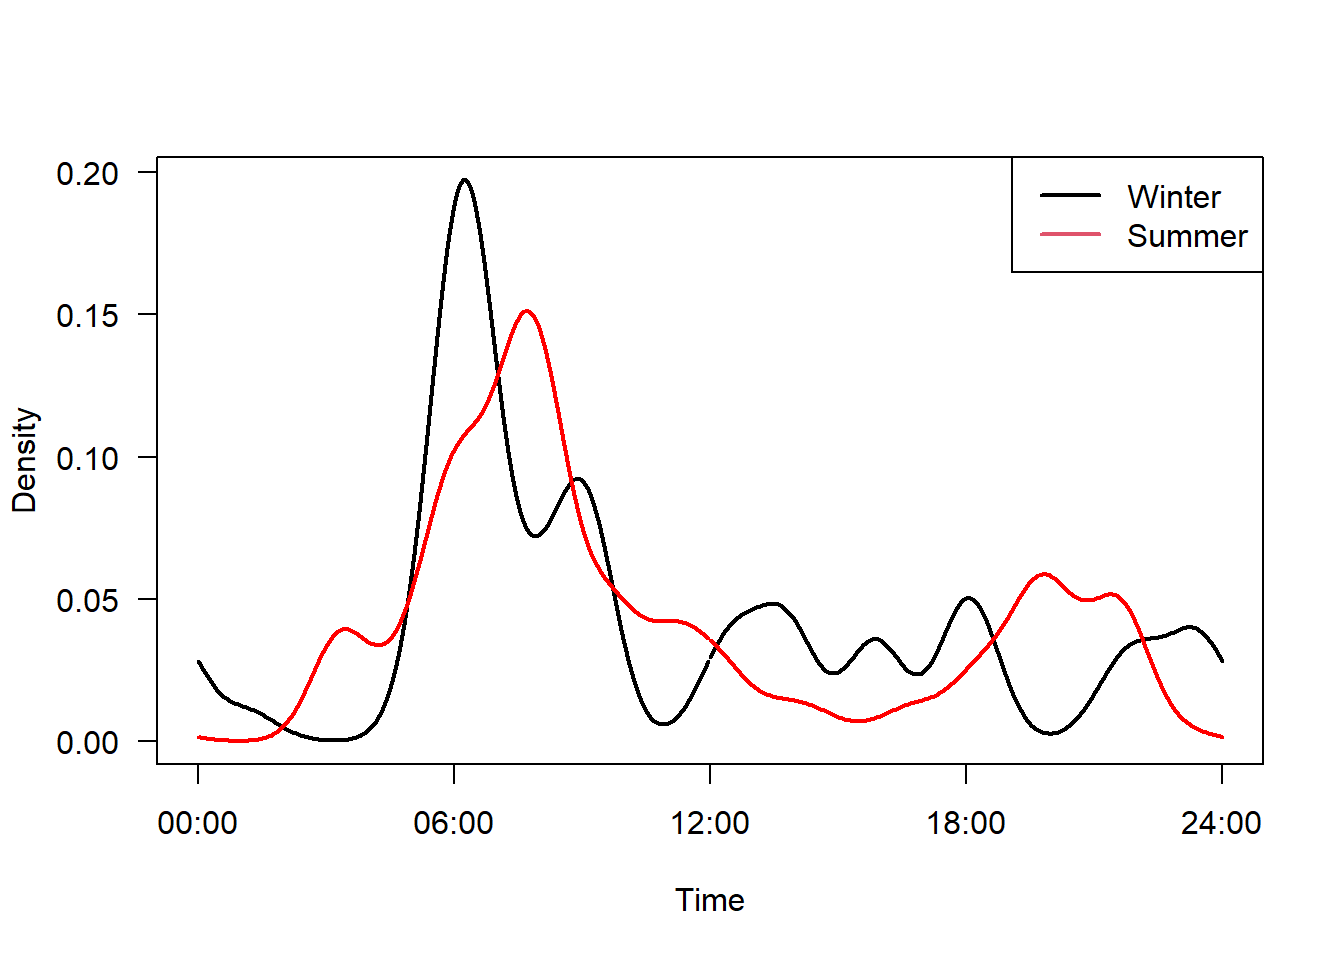
\includegraphics{bookdown-demo_files/figure-latex/unnamed-chunk-20-1.pdf}

\textbf{Multiple strata}

The code to build a multi strata comparison is very similar to that of a
single strata, except now you separate the observations into their
relevent categories. To make this split, we refer to the \texttt{sta}
dataframe, which contains the treatment types for each camera station.
We match the Deployment.Location.ID's in our dataframe with those in
each treatment category using the \texttt{\%in\%} command.

\begin{Shaded}
\begin{Highlighting}[]
\CommentTok{# The treatment types for each Deployment.Location.ID are in the sta file}
\CommentTok{# Make an object containing all of the site ID's for the "Offline" cameras}
\NormalTok{off <-}\StringTok{ }\NormalTok{sta}\OperatorTok{$}\NormalTok{Deployment.Location.ID[sta}\OperatorTok{$}\NormalTok{Treatment}\OperatorTok{==}\StringTok{"Offline"}\NormalTok{]}
\CommentTok{# And "HumanUse" cameras}
\NormalTok{hum <-}\StringTok{ }\NormalTok{sta}\OperatorTok{$}\NormalTok{Deployment.Location.ID[sta}\OperatorTok{$}\NormalTok{Treatment}\OperatorTok{==}\StringTok{"HumanUse"}\NormalTok{]}

\CommentTok{# Create a new empty list}
\NormalTok{strata <-}\StringTok{ }\KeywordTok{list}\NormalTok{()}

\CommentTok{# Only sum the data for each relvent strata}
\NormalTok{strata[[}\DecValTok{1}\NormalTok{]] <-}\StringTok{ }\KeywordTok{colSums}\NormalTok{(totObs[totObs}\OperatorTok{$}\NormalTok{Deployment.Location.ID }\OperatorTok\StringTok{ }\NormalTok{off, }\DecValTok{3}\OperatorTok{:}\KeywordTok{ncol}\NormalTok{(totObs)])}
\NormalTok{strata[[}\DecValTok{2}\NormalTok{]] <-}\StringTok{ }\KeywordTok{colSums}\NormalTok{(totObs[totObs}\OperatorTok{$}\NormalTok{Deployment.Location.ID }\OperatorTok\StringTok{ }\NormalTok{hum, }\DecValTok{3}\OperatorTok{:}\KeywordTok{ncol}\NormalTok{(totObs)])}

\CommentTok{# Give them names}
\KeywordTok{names}\NormalTok{(strata) <-}\StringTok{ }\KeywordTok{c}\NormalTok{(}\StringTok{"Offline"}\NormalTok{, }\StringTok{"HumanUse"}\NormalTok{)}
\end{Highlighting}
\end{Shaded}

Then, as before, run your iNEXT model and examine the output:

\begin{Shaded}
\begin{Highlighting}[]
\NormalTok{out <-}\StringTok{ }\KeywordTok{iNEXT}\NormalTok{(strata, }\DataTypeTok{datatype=}\StringTok{"abundance"}\NormalTok{)}
\NormalTok{p1 <-}\StringTok{ }\KeywordTok{ggiNEXT}\NormalTok{(out, }\DataTypeTok{type=}\DecValTok{1}\NormalTok{)}\OperatorTok{+}\StringTok{ }\KeywordTok{theme_classic}\NormalTok{() }
\NormalTok{p2 <-}\StringTok{ }\KeywordTok{ggiNEXT}\NormalTok{(out, }\DataTypeTok{type=}\DecValTok{2}\NormalTok{)}\OperatorTok{+}\StringTok{ }\KeywordTok{theme_classic}\NormalTok{() }
\KeywordTok{grid.arrange}\NormalTok{(p1, p2, }\DataTypeTok{nrow =} \DecValTok{1}\NormalTok{)}
\end{Highlighting}
\end{Shaded}

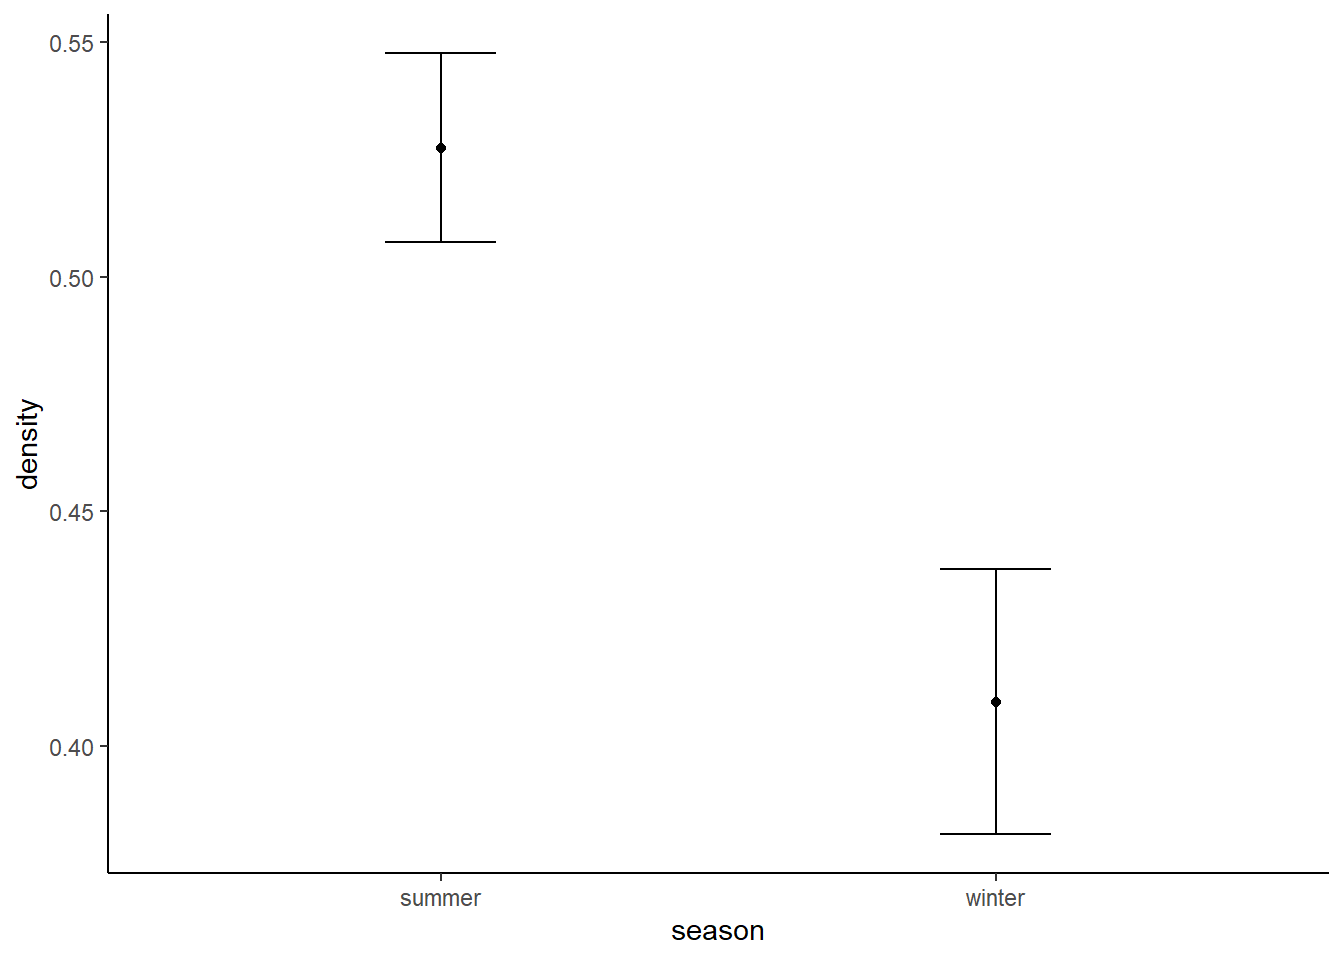
\includegraphics{bookdown-demo_files/figure-latex/unnamed-chunk-22-1.pdf}

From the plot on the left you can see that the `HumanUse' strata
detected more species than the `Offline' strata. The plot on the right
suggests that we have likely sampled all of the species that will be
detected within these habitats (samples are `complete').

\textbf{Notes} These two examples just scratch the surface of the
functionality of the iNEXT package, and the ways of using it with camera
data.

\textbf{Examples}

Some examples of using iNEXT with camera trap data:

\href{https://journals.plos.org/plosone/article?id=10.1371/journal.pone.0126373}{Cusack
et.al 2015} Random versus Game Trail-Based Camera Trap Placement
Strategy for Monitoring Terrestrial Mammal Communities

\subsection{Multispecies occupancy
model}\label{multispecies-occupancy-model}

It is also possible to estimate species richness in a given area/strata
using multispecies occupancy models. Move through to \textbf{THE
OCCUPANCY MODEL SECTION} if this is the path you want to go down!

\section{Diversity}\label{diversity}

One issue with species richness assessments is that they weight all
species equally, thus a community with 12 species all present in equal
abundances will give you the same richness value as a high skewed
community with one highly abundant species, and 11 very rare ones.
Consequently, you might want to estimate species diversity.

Luckily, the iNEXT package is well suited for comparisons of diversity
indices through the use of hill numbers - of which the `q' value
represents the traditional shannon (q=1) and simpson (q=2) diversity
indices (species richness: q = 0). \emph{Note} Increasing values of q
reduces the influence of rare species on your estimate of community
diversity.

For example, we might want to compare the species diversity accross our
two focal strata:

\begin{Shaded}
\begin{Highlighting}[]
\CommentTok{# We also introduce the object t -> which reflects the range of values over which you want to predict species richness}
\NormalTok{t <-}\StringTok{ }\KeywordTok{c}\NormalTok{(}\DecValTok{1}\NormalTok{, }\KeywordTok{seq}\NormalTok{(}\DecValTok{2}\NormalTok{, }\DecValTok{300}\NormalTok{, }\DataTypeTok{by=}\DecValTok{2}\NormalTok{))}
\CommentTok{# For q =2 (shannon)}
\NormalTok{out <-}\StringTok{ }\KeywordTok{iNEXT}\NormalTok{(strata, }\DataTypeTok{q=}\KeywordTok{c}\NormalTok{(}\DecValTok{1}\NormalTok{,}\DecValTok{2}\NormalTok{) ,}\DataTypeTok{datatype=}\StringTok{"abundance"}\NormalTok{, }\DataTypeTok{size=}\NormalTok{t)}
\KeywordTok{ggiNEXT}\NormalTok{(out, }\DataTypeTok{type=}\DecValTok{1}\NormalTok{, }\DataTypeTok{facet.var=}\StringTok{"order"}\NormalTok{, }\DataTypeTok{color.var=}\StringTok{"site"}\NormalTok{) }\OperatorTok{+}\StringTok{ }\KeywordTok{theme_classic}\NormalTok{() }
\end{Highlighting}
\end{Shaded}

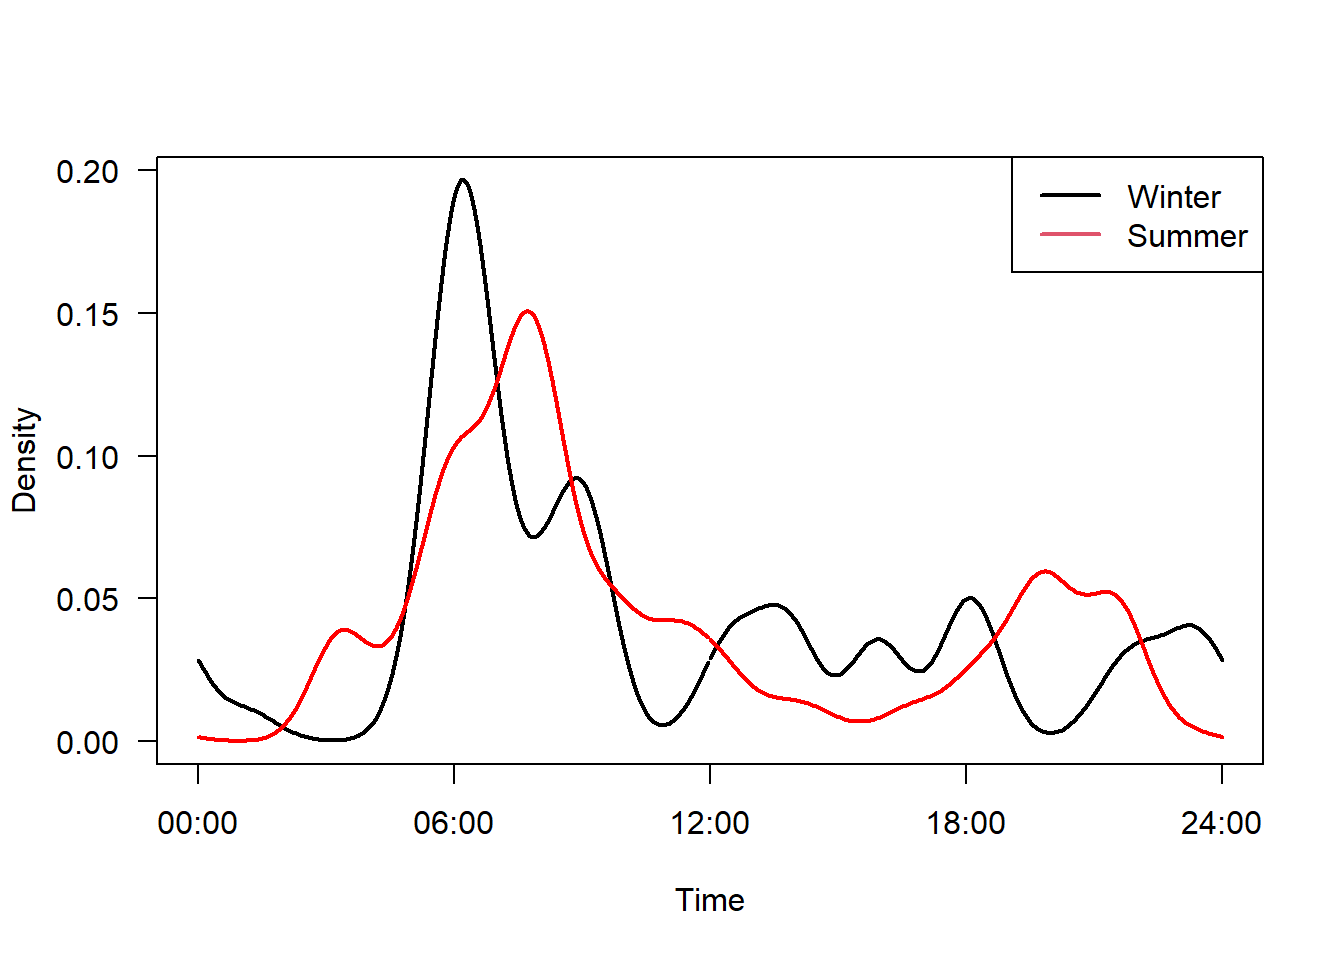
\includegraphics{bookdown-demo_files/figure-latex/unnamed-chunk-23-1.pdf}

The plot above shows that the differences between our two strata remain
across increasing q values (suggesting that the different inst just
driven by several rarely encountered species).

Point estimates and their confidence intervals can also be extracted
from iNEXT model objects - but it does require a little data wrangling.
For example, if we wanted to directly compare the diversity estimates of
our strata at 250 individuals:

\begin{Shaded}
\begin{Highlighting}[]
\CommentTok{# The lapply function applies the same logic across elements in a list}
\NormalTok{point.}\DecValTok{250}\NormalTok{ <-}\StringTok{ }\KeywordTok{lapply}\NormalTok{(out}\OperatorTok{$}\NormalTok{iNextEst, }\ControlFlowTok{function}\NormalTok{(x) \{ x[ x}\OperatorTok{$}\NormalTok{m }\OperatorTok{==}\StringTok{ }\DecValTok{250}\NormalTok{, ] \})}
\CommentTok{# Turn the output into a dataframe}
\NormalTok{point.df <-}\StringTok{ }\KeywordTok{do.call}\NormalTok{(rbind, point.}\DecValTok{250}\NormalTok{)}
\CommentTok{# Extract the strata}
\NormalTok{point.df}\OperatorTok{$}\NormalTok{Strata <-}\StringTok{ }\KeywordTok{gsub}\NormalTok{(}\StringTok{"}\CharTok{\textbackslash{}\textbackslash{}}\StringTok{..*"}\NormalTok{,}\StringTok{""}\NormalTok{,}\KeywordTok{rownames}\NormalTok{(point.df))}

\NormalTok{q.vals <-}\StringTok{ }\KeywordTok{c}\NormalTok{(}\StringTok{"test"}\NormalTok{, }\StringTok{"why"}\NormalTok{)}
\NormalTok{point.df}\OperatorTok{$}\NormalTok{order <-}\StringTok{ }\KeywordTok{as.factor}\NormalTok{(point.df}\OperatorTok{$}\NormalTok{order)}
\CommentTok{# Make a nice ggplot!}
\KeywordTok{ggplot}\NormalTok{(point.df, }\KeywordTok{aes}\NormalTok{(}\DataTypeTok{x=}\NormalTok{order, }\DataTypeTok{y=}\NormalTok{qD, }\DataTypeTok{colour=}\NormalTok{Strata)) }\OperatorTok{+}\StringTok{ }
\StringTok{    }\KeywordTok{theme_classic}\NormalTok{() }\OperatorTok{+}
\StringTok{    }\CommentTok{#scale_x_discrete(breaks=c("1","2"),labels= c("1","2")) +}
\StringTok{    }\KeywordTok{geom_errorbar}\NormalTok{(}\KeywordTok{aes}\NormalTok{(}\DataTypeTok{ymin=}\NormalTok{qD.LCL, }\DataTypeTok{ymax=}\NormalTok{qD.UCL), }\DataTypeTok{width=}\NormalTok{.}\DecValTok{01}\NormalTok{) }\OperatorTok{+}
\StringTok{    }\KeywordTok{labs}\NormalTok{(}\DataTypeTok{y=}\StringTok{"Diversity"}\NormalTok{, }\DataTypeTok{x =} \StringTok{"q Value"}\NormalTok{) }\OperatorTok{+}
\StringTok{    }\KeywordTok{geom_point}\NormalTok{() }
\end{Highlighting}
\end{Shaded}

\includegraphics{bookdown-demo_files/figure-latex/unnamed-chunk-24-1.pdf}

\section{Trait diversity}\label{trait-diversity}

\section{Limitations to consider}\label{limitations-to-consider}

TBC

\chapter{Habitat use}\label{habitat-use}

Camera traps are well suited for the quantification of habitat use
accross multiple species. To assess habitat use, we typically quantify
the detection rate, or a relative abundance index (RAI). RAI estimates
are fairly simple to estimate, and understand, than other metrics (such
as occupancy)and thus their use is widespread.

In its simpliest form this represents the number of indpendent events
(or individuals within indepnendent events) of a given species at a
given camera, divided by the number of days that camera was active
during that period of interest.

Such abundance indices are typically analysed in a linear modelling
framework, for single species, increasingly, for multispecies
assemblages. Addressed in turn below.

We will use the
``processed\_data/Algar\_30min\_Independent\_Monthly\_counts.csv''
dataframe as the starting point for this data analysis. Which looks like
this:

\begin{Shaded}
\begin{Highlighting}[]
\NormalTok{monCount <-}\StringTok{ }\KeywordTok{read.csv}\NormalTok{(}\StringTok{"data/processed_data/Algar_30min_Independent_Monthly_counts.csv"}\NormalTok{, }\DataTypeTok{header=}\NormalTok{T)}
\end{Highlighting}
\end{Shaded}

Which, as a quick reminder, looks like this:

\begin{table}
\centering
\begin{tabular}[t]{l|l|r|r|r|r|r|r|r|r|r|r|r|r|r}
\hline
Deployment.Location.ID & Date & Effort & Alces.alces & Canis.latrans & Canis.lupus & Cervus.canadensis & Grus.canadensis & Lepus.americanus & Lynx.canadensis & Martes.americana & Odocoileus.virginianus & Rangifer.tarandus & Tamiasciurus.hudsonicus & Ursus.americanus\\
\hline
Algar08 & 2018-11 & 14 & 0 & 0 & 0 & 0 & 0 & 0 & 0 & 0 & 0 & 0 & 0 & 0\\
\hline
Algar08 & 2018-12 & 31 & 0 & 0 & 0 & 0 & 0 & 0 & 0 & 0 & 1 & 0 & 0 & 0\\
\hline
Algar08 & 2019-01 & 31 & 0 & 0 & 0 & 0 & 0 & 0 & 0 & 0 & 0 & 0 & 0 & 0\\
\hline
Algar08 & 2019-02 & 28 & 0 & 0 & 0 & 0 & 0 & 0 & 0 & 0 & 0 & 0 & 0 & 0\\
\hline
Algar08 & 2019-03 & 31 & 0 & 0 & 0 & 0 & 0 & 0 & 0 & 0 & 0 & 0 & 0 & 0\\
\hline
Algar08 & 2019-04 & 30 & 4 & 0 & 0 & 0 & 0 & 0 & 0 & 0 & 0 & 0 & 0 & 0\\
\hline
\end{tabular}
\end{table}

So our rows represent a month at each given site, and we have the number
of camera days each location was trapped. This is also the format which
most liner model analysis packages require you to have your data in.
Easy!

Our next step to create the relative abundance index. We will divide
each count by the number of days the station was active in each month
then multiply by the a standardised number of days - often people use
100.

In R this would look like:

\begin{Shaded}
\begin{Highlighting}[]
\CommentTok{# Create a dataframe to store these 'relative abundances'}
\NormalTok{monRAI <-}\StringTok{ }\NormalTok{monCount}
\CommentTok{# Divide the species abundances (which start in column four), by the amount of camera effort}
\NormalTok{monRAI[ , }\DecValTok{4}\OperatorTok{:}\KeywordTok{ncol}\NormalTok{(monCount)] <-}\StringTok{ }\NormalTok{(monRAI[ , }\DecValTok{4}\OperatorTok{:}\KeywordTok{ncol}\NormalTok{(monCount)]}\OperatorTok{/}\NormalTok{monRAI}\OperatorTok{$}\NormalTok{Effort)}\OperatorTok{*}\DecValTok{100}
\end{Highlighting}
\end{Shaded}

We can then examine the relationship between raw counts (on the x-axis)
with our relative abundance index (on the y-axis), using
\emph{Odocoileus virginianus} as an example:

\begin{Shaded}
\begin{Highlighting}[]
\KeywordTok{plot}\NormalTok{(monRAI}\OperatorTok{$}\NormalTok{Odocoileus.virginianus }\OperatorTok{~}\StringTok{ }\NormalTok{monCount}\OperatorTok{$}\NormalTok{Odocoileus.virginianus,}
     \DataTypeTok{las=}\DecValTok{1}\NormalTok{, }\DataTypeTok{pch=}\DecValTok{19}\NormalTok{, }\DataTypeTok{ylab=}\StringTok{"RAI"}\NormalTok{, }\DataTypeTok{xlab=}\StringTok{"Raw"}\NormalTok{)}
\KeywordTok{abline}\NormalTok{(}\DataTypeTok{a=}\DecValTok{0}\NormalTok{, }\DataTypeTok{b=}\FloatTok{3.22}\NormalTok{, }\DataTypeTok{lty=}\DecValTok{2}\NormalTok{, }\DataTypeTok{col=}\StringTok{"grey"}\NormalTok{)}
\end{Highlighting}
\end{Shaded}

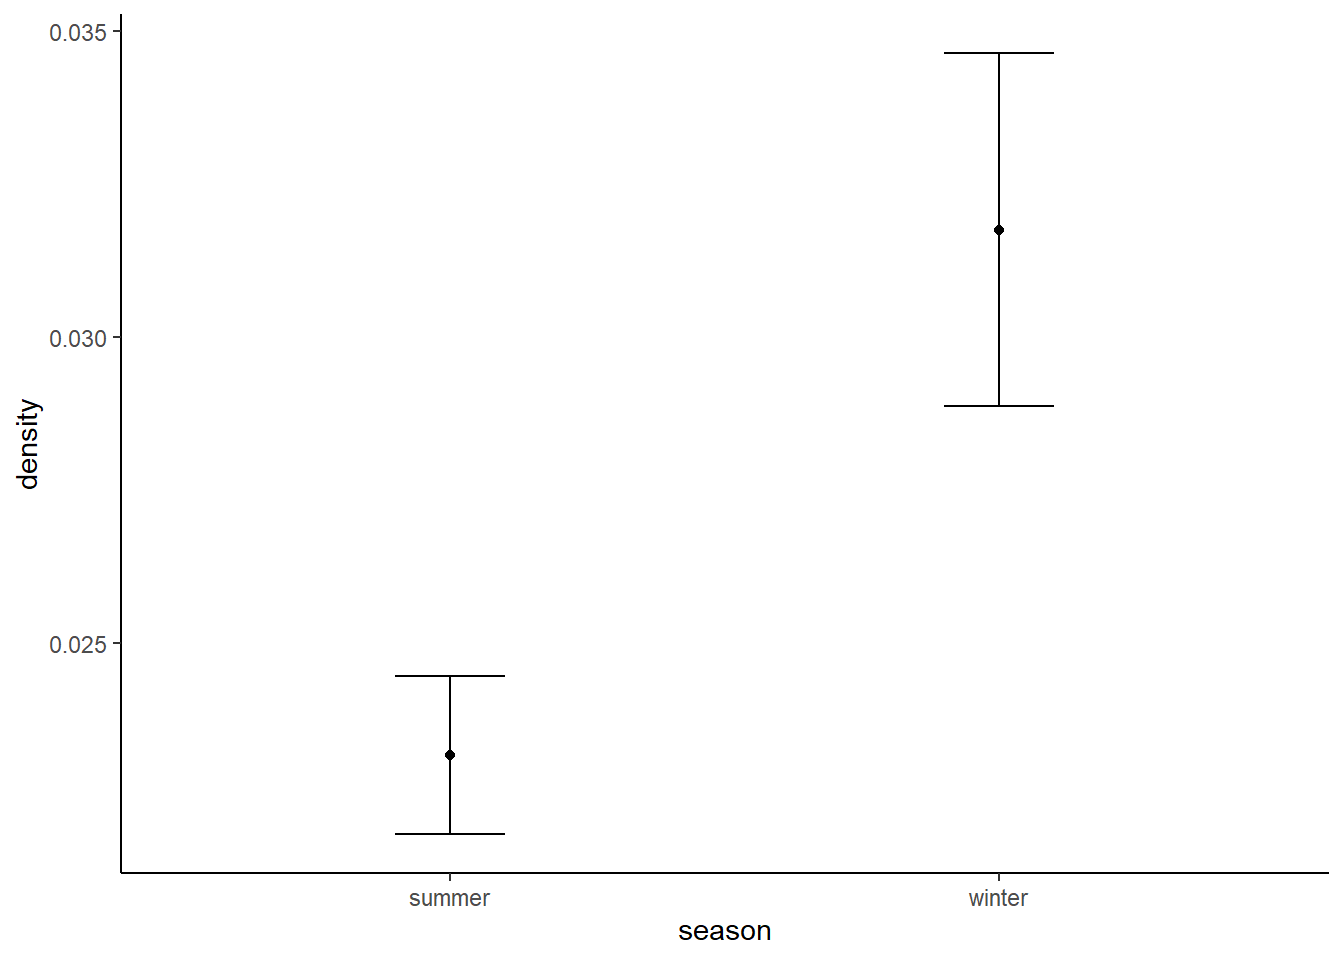
\includegraphics{bookdown-demo_files/figure-latex/unnamed-chunk-29-1.pdf}

So in months where we have an incomplete sample (say 20 days in January
instead of 31), the RAI will be higher than the dashed grey line.

\section{Single species habitat use
model}\label{single-species-habitat-use-model}

The most common way to analyse habitat use data is through linear
models. There are a variety if differnt frameworks to fit and compare
different linear models to address a host of different hypotheses, but
if you are just starting out you should be aware of two key packages:

\begin{itemize}
\tightlist
\item
  \texttt{lme4} -\textgreater{} frequentist and information theoretic
  approaches
\item
  \texttt{brms} -\textgreater{} bayseian approaches
\end{itemize}

There is no right or wrong about which package and which approach you
use to test your hypotheses, just make sure you understand the
implications of your choices!

\textbf{RESOURCES To Go HERE}

\textbf{Example in lme4}

In this worked example we will analyse how mammal capture vary using a
mixed effects model. We will not test the model assumptions or
interograte the findings, there are better resources to allow you to do
that! Here we simply demonstrate how to use our camera datat to fit the
model.

First we must install the packages we require: `lme4' and `tidyr':

\begin{Shaded}
\begin{Highlighting}[]
 \KeywordTok{library}\NormalTok{(lme4); }\KeywordTok{library}\NormalTok{(tidyr)}
\end{Highlighting}
\end{Shaded}

The lme4 package requires a dataframe format (as above), with the
response term and the predictor variables all included in the same
location. In this example we will explore if the habitat use of
\emph{Odocoileus virginianus} varied based on treatment strata.

\textbf{Preparing our data}

Recall that the information about each camera is recorded in the
Station\_covariares file:

\begin{Shaded}
\begin{Highlighting}[]
\NormalTok{sta <-}\StringTok{ }\KeywordTok{read.csv}\NormalTok{(}\StringTok{"data/raw_data/Example_station_data.csv"}\NormalTok{, }\DataTypeTok{header=}\NormalTok{T)}

\KeywordTok{kbl}\NormalTok{(}\KeywordTok{head}\NormalTok{(sta))}\OperatorTok
\StringTok{  }\KeywordTok{kable_paper}\NormalTok{() }\OperatorTok
\StringTok{  }\KeywordTok{scroll_box}\NormalTok{(}\DataTypeTok{width =} \StringTok{"750px"}\NormalTok{, }\DataTypeTok{height =} \StringTok{"200px"}\NormalTok{)}
\end{Highlighting}
\end{Shaded}

\begin{table}
\centering
\begin{tabular}[t]{l|r|r|l|r|r}
\hline
Deployment.Location.ID & Longitude & Latitude & Treatment & LOW500 & LOS\\
\hline
Algar08 & -112.4152 & 56.24259 & HumanUse & 0.3991810 & 112.7500\\
\hline
Algar27 & -112.4735 & 56.33280 & HumanUse & 0.8345277 & 252.9583\\
\hline
Algar29 & -112.5483 & 56.39474 & HumanUse & 0.6542558 & 206.5278\\
\hline
Algar31 & -112.4820 & 56.30899 & HumanUse & 0.6180393 & 334.2778\\
\hline
Algar32 & -112.3968 & 56.40197 & HumanUse & 0.5678142 & 83.0000\\
\hline
Algar34 & -112.4012 & 56.22248 & HumanUse & 0.5492762 & 337.7917\\
\hline
\end{tabular}
\end{table}

So we have three variables to pick from:

\begin{itemize}
\tightlist
\item
  \texttt{Treatment} is the feature where the camera trap was deployed:
  HumanUse = a camera on a seismic line used and maintained in an
  ``open'' state by humans; Offline = a camera in contiguous forest
  \textgreater{}200m from a seismic line\\
\item
  \texttt{LOW500} is the proportion of surrounding habitat 500m around
  the camera which is classified as ``Lowland''
\item
  \texttt{LOS} is the average straight line distance in m which you can
  view from the camera trap location.
\end{itemize}

In this example we will start by keeping things simple and just
exploring if \texttt{LOW500} influences the habitat use of
\emph{Odocoileus virginianus}.

Our first task is to link the information in the \texttt{sta} dataframe,
with that in the monCount dataframe. To do this we will use
\texttt{left\_join()} in the dplyr package - using the camera stations
(\texttt{Deployment.Location.ID} column) to link the data.

\begin{Shaded}
\begin{Highlighting}[]
\KeywordTok{library}\NormalTok{(dplyr)}
\NormalTok{modDat <-}\StringTok{ }\KeywordTok{left_join}\NormalTok{(monCount, sta[}\KeywordTok{c}\NormalTok{(}\StringTok{"Deployment.Location.ID"}\NormalTok{, }\StringTok{"LOW500"}\NormalTok{)])}
\end{Highlighting}
\end{Shaded}

\begin{verbatim}
## Joining, by = "Deployment.Location.ID"
\end{verbatim}

Lets check it has worked, the \texttt{LOW500} column should be added on
the right hand side:

\begin{Shaded}
\begin{Highlighting}[]
\KeywordTok{kbl}\NormalTok{(}\KeywordTok{head}\NormalTok{(modDat))}\OperatorTok
\StringTok{  }\KeywordTok{kable_paper}\NormalTok{() }\OperatorTok
\StringTok{  }\KeywordTok{scroll_box}\NormalTok{(}\DataTypeTok{width =} \StringTok{"750px"}\NormalTok{, }\DataTypeTok{height =} \StringTok{"200px"}\NormalTok{)}
\end{Highlighting}
\end{Shaded}

\begin{table}
\centering
\begin{tabular}[t]{l|l|r|r|r|r|r|r|r|r|r|r|r|r|r|r}
\hline
Deployment.Location.ID & Date & Effort & Alces.alces & Canis.latrans & Canis.lupus & Cervus.canadensis & Grus.canadensis & Lepus.americanus & Lynx.canadensis & Martes.americana & Odocoileus.virginianus & Rangifer.tarandus & Tamiasciurus.hudsonicus & Ursus.americanus & LOW500\\
\hline
Algar08 & 2018-11 & 14 & 0 & 0 & 0 & 0 & 0 & 0 & 0 & 0 & 0 & 0 & 0 & 0 & 0.399181\\
\hline
Algar08 & 2018-12 & 31 & 0 & 0 & 0 & 0 & 0 & 0 & 0 & 0 & 1 & 0 & 0 & 0 & 0.399181\\
\hline
Algar08 & 2019-01 & 31 & 0 & 0 & 0 & 0 & 0 & 0 & 0 & 0 & 0 & 0 & 0 & 0 & 0.399181\\
\hline
Algar08 & 2019-02 & 28 & 0 & 0 & 0 & 0 & 0 & 0 & 0 & 0 & 0 & 0 & 0 & 0 & 0.399181\\
\hline
Algar08 & 2019-03 & 31 & 0 & 0 & 0 & 0 & 0 & 0 & 0 & 0 & 0 & 0 & 0 & 0 & 0.399181\\
\hline
Algar08 & 2019-04 & 30 & 4 & 0 & 0 & 0 & 0 & 0 & 0 & 0 & 0 & 0 & 0 & 0 & 0.399181\\
\hline
\end{tabular}
\end{table}

Next we will fit a mixed effects model to this dataset using
\texttt{lme4}. You may have noticed that we havent used the monRAI
dataframe we fit earlier! That is because we can create a relative
abundance index within the model itself by providing an
\texttt{offset()} - which functions in an equivalent way to what we did
beforehand, and preseveres the original units of the obsevations
(counts).

The model takes the form:

Response term \textasciitilde{} fixed effect + offset +
(1\textbar{}random intercept), data frame, distribution

We include \texttt{Deployment.Locaion.ID} as the random intercept, as
camera stations are repeatedly sampled at monthly intervals and thus our
data (rows in the dataframe) are not independent. We use the
\texttt{poisson} family, as our response term is a count.

\begin{Shaded}
\begin{Highlighting}[]
\NormalTok{m1 <-}\StringTok{ }\KeywordTok{glmer}\NormalTok{(Odocoileus.virginianus }\OperatorTok{~}\StringTok{ }\NormalTok{LOW500 }\OperatorTok{+}\StringTok{ }\KeywordTok{offset}\NormalTok{(}\KeywordTok{log}\NormalTok{(Effort)) }\OperatorTok{+}\StringTok{ }\NormalTok{(}\DecValTok{1}\OperatorTok{|}\NormalTok{Deployment.Location.ID) , }\DataTypeTok{data=}\NormalTok{modDat, }\DataTypeTok{family=}\StringTok{"poisson"}\NormalTok{)}
\end{Highlighting}
\end{Shaded}

We can view a summary of the model fit using:

\begin{Shaded}
\begin{Highlighting}[]
\KeywordTok{summary}\NormalTok{(m1)}
\end{Highlighting}
\end{Shaded}

\begin{verbatim}
## Generalized linear mixed model fit by maximum likelihood (Laplace
##   Approximation) [glmerMod]
##  Family: poisson  ( log )
## Formula: Odocoileus.virginianus ~ LOW500 + offset(log(Effort)) + (1 |  
##     Deployment.Location.ID)
##    Data: modDat
## 
##      AIC      BIC   logLik deviance df.resid 
##    540.8    551.3   -267.4    534.8      245 
## 
## Scaled residuals: 
##     Min      1Q  Median      3Q     Max 
## -2.1896 -0.4391 -0.2499 -0.1293  4.2043 
## 
## Random effects:
##  Groups                 Name        Variance Std.Dev.
##  Deployment.Location.ID (Intercept) 4.002    2       
## Number of obs: 248, groups:  Deployment.Location.ID, 20
## 
## Fixed effects:
##             Estimate Std. Error z value Pr(>|z|)  
## (Intercept)   -1.957      1.778  -1.101   0.2710  
## LOW500        -4.807      2.598  -1.850   0.0643 .
## ---
## Signif. codes:  0 '***' 0.001 '**' 0.01 '*' 0.05 '.' 0.1 ' ' 1
## 
## Correlation of Fixed Effects:
##        (Intr)
## LOW500 -0.953
\end{verbatim}

As stated at the start of this guide, we are not focusing on whether the
models we apply are appropriate or finding ``the best'' models for this
datatset, so do not spend too much time trying to interpret this
infomation!

We can plot the relationship between by keeping things simple and just
exploring if \texttt{LOW500} influences the habitat use of
\emph{Odocoileus virginianus} habitat using the predict function and
\texttt{ggplot2}.

\begin{Shaded}
\begin{Highlighting}[]
\NormalTok{newDat <-}\StringTok{ }\KeywordTok{cbind}\NormalTok{(}\KeywordTok{expand.grid}\NormalTok{(}\DataTypeTok{LOW500=}\KeywordTok{seq}\NormalTok{(}\KeywordTok{min}\NormalTok{(sta}\OperatorTok{$}\NormalTok{LOW500),}\KeywordTok{max}\NormalTok{(sta}\OperatorTok{$}\NormalTok{LOW500), }\DataTypeTok{length.out=}\DecValTok{50}\NormalTok{)),}\DataTypeTok{Effort=}\DecValTok{100}\NormalTok{)}

\CommentTok{# Type "response" gives predictions on the original (count) scale.}
\NormalTok{newDat}\OperatorTok{$}\NormalTok{Pred <-}\StringTok{ }\KeywordTok{predict}\NormalTok{(m1,}\DataTypeTok{newdata=}\NormalTok{newDat,}\DataTypeTok{re.form=}\OtherTok{NA}\NormalTok{,}
                  \DataTypeTok{type=}\StringTok{"response"}\NormalTok{)}

\KeywordTok{plot}\NormalTok{(newDat}\OperatorTok{$}\NormalTok{Pred}\OperatorTok{~}\NormalTok{newDat}\OperatorTok{$}\NormalTok{LOW500, }\DataTypeTok{type=}\StringTok{"l"}\NormalTok{,}
     \DataTypeTok{ylim=}\KeywordTok{c}\NormalTok{(}\DecValTok{0}\NormalTok{, }\KeywordTok{max}\NormalTok{(newDat}\OperatorTok{$}\NormalTok{Pred)), }\DataTypeTok{lwd=}\DecValTok{2}\NormalTok{,}
     \DataTypeTok{las=}\DecValTok{1}\NormalTok{, }\DataTypeTok{ylab=}\StringTok{"Predicted habitat use"}\NormalTok{,}
     \DataTypeTok{xlab=}\StringTok{"Proportion lowland habitat"}\NormalTok{)}
\end{Highlighting}
\end{Shaded}

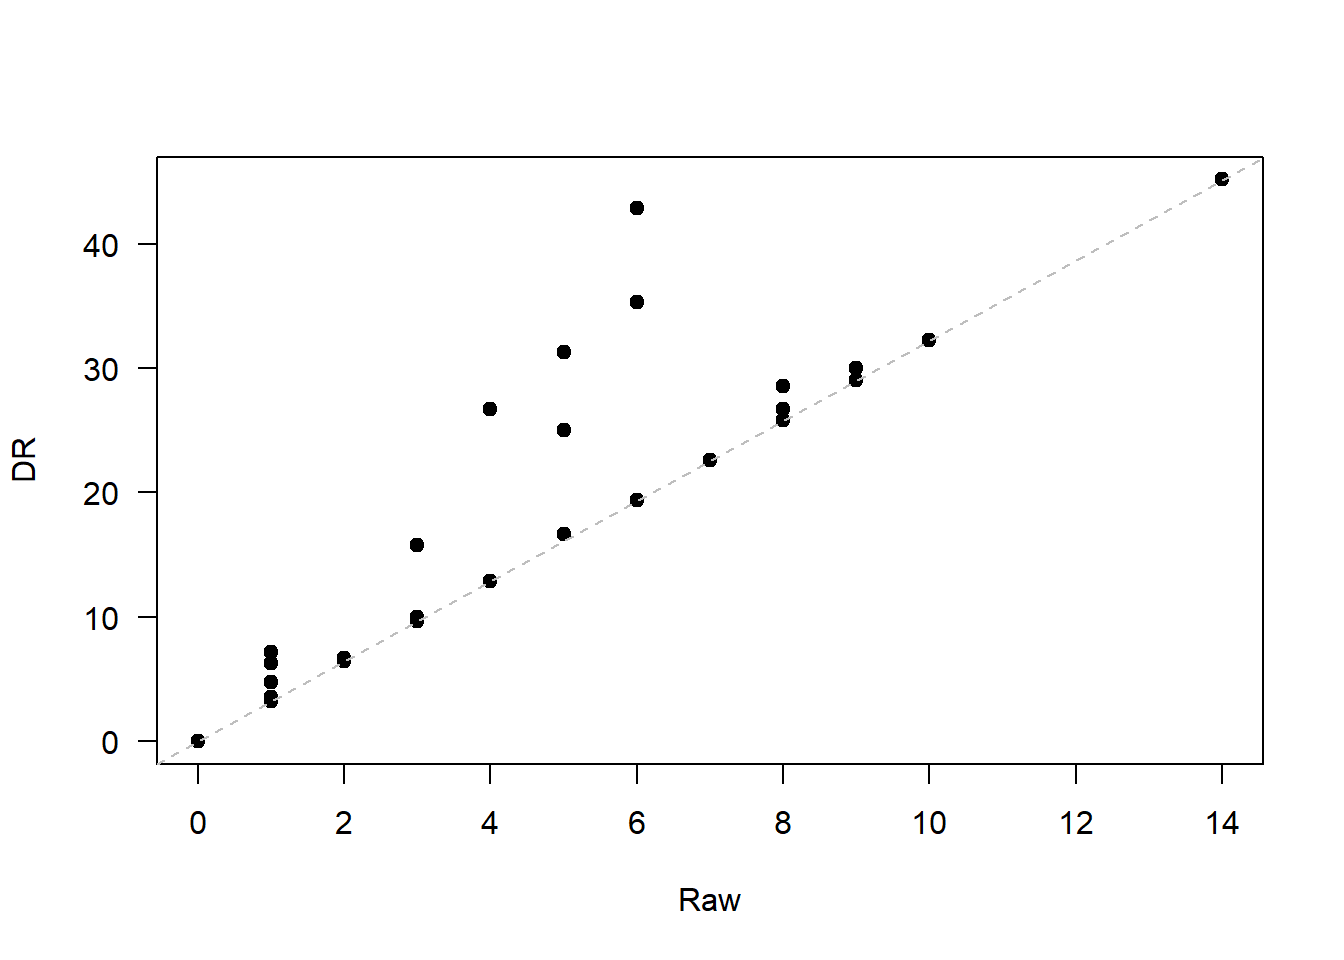
\includegraphics{bookdown-demo_files/figure-latex/unnamed-chunk-36-1.pdf}

So our model suggests that the habitat use of \emph{Odocoileus
virginianus} decreases as the proportion of loaland habitat increases.
This is consistent with our understanding of White-tailed deer, which
prefer upland habitats!

If you want more applied examples of generating predictions from mixed
effects models, check out
\href{https://bbolker.github.io/mixedmodels-misc/ecostats_chap.html}{Ben
Bolkers workbook}

\section{Further things to consider}\label{further-things-to-consider}

\begin{itemize}
\tightlist
\item
  bayesian models - brms materials
\item
  model fit
\item
  overdispersion
\item
  standardising input variables
\end{itemize}

\section{Example multispecies model}\label{example-multispecies-model}

Given advances in computer power and analytic approaches, it is becoming
increasingly popular to model multiple species within the same
frameowrk. This opens up a variety of things not previously possible.

As with single species linear models, there are many choices available
for modeeling multiple species in the same frameowrk. Two notable
options are:

\begin{itemize}
\tightlist
\item
  GJAM
\item
  HMSc
\end{itemize}

In this example we will use the \texttt{Hmsc} package.

\begin{Shaded}
\begin{Highlighting}[]
\KeywordTok{library}\NormalTok{(Hmsc)}
\end{Highlighting}
\end{Shaded}

\textbf{Preparing our data}

The format of data required for joint species distribution models is
different to that of traditional linear models.

Rather than lumping the response term and fixed effects within the the
same dataframe, we need a separate \texttt{Y} matrix of site.time x
species, and an \texttt{Xdata} dataframe of your fixed and random
effects variables.

\begin{Shaded}
\begin{Highlighting}[]
\CommentTok{# Pull the count data into its own matrix}
\NormalTok{Y <-}\StringTok{ }\KeywordTok{as.matrix}\NormalTok{(monCount[, }\DecValTok{4}\OperatorTok{:}\KeywordTok{ncol}\NormalTok{(monCount)])}
\CommentTok{# You can make the rown names the Site.Date values }
\CommentTok{# (just incase you want to check things)}
\KeywordTok{row.names}\NormalTok{(Y) <-}\StringTok{ }\KeywordTok{paste}\NormalTok{(monCount}\OperatorTok{$}\NormalTok{Deployment.Location.ID, monCount}\OperatorTok{$}\NormalTok{Date, }\DataTypeTok{sep=}\StringTok{"."}\NormalTok{)}
\end{Highlighting}
\end{Shaded}

Which looks like this:

\begin{Shaded}
\begin{Highlighting}[]
\KeywordTok{kbl}\NormalTok{(}\KeywordTok{head}\NormalTok{(Y))}\OperatorTok
\StringTok{  }\KeywordTok{kable_paper}\NormalTok{() }\OperatorTok
\StringTok{  }\KeywordTok{scroll_box}\NormalTok{(}\DataTypeTok{width =} \StringTok{"750px"}\NormalTok{, }\DataTypeTok{height =} \StringTok{"200px"}\NormalTok{)}
\end{Highlighting}
\end{Shaded}

\begin{table}
\centering
\begin{tabular}[t]{l|r|r|r|r|r|r|r|r|r|r|r|r}
\hline
  & Alces.alces & Canis.latrans & Canis.lupus & Cervus.canadensis & Grus.canadensis & Lepus.americanus & Lynx.canadensis & Martes.americana & Odocoileus.virginianus & Rangifer.tarandus & Tamiasciurus.hudsonicus & Ursus.americanus\\
\hline
Algar08.2018-11 & 0 & 0 & 0 & 0 & 0 & 0 & 0 & 0 & 0 & 0 & 0 & 0\\
\hline
Algar08.2018-12 & 0 & 0 & 0 & 0 & 0 & 0 & 0 & 0 & 1 & 0 & 0 & 0\\
\hline
Algar08.2019-01 & 0 & 0 & 0 & 0 & 0 & 0 & 0 & 0 & 0 & 0 & 0 & 0\\
\hline
Algar08.2019-02 & 0 & 0 & 0 & 0 & 0 & 0 & 0 & 0 & 0 & 0 & 0 & 0\\
\hline
Algar08.2019-03 & 0 & 0 & 0 & 0 & 0 & 0 & 0 & 0 & 0 & 0 & 0 & 0\\
\hline
Algar08.2019-04 & 4 & 0 & 0 & 0 & 0 & 0 & 0 & 0 & 0 & 0 & 0 & 0\\
\hline
\end{tabular}
\end{table}

We then create the XData in a similar way to before, but this time
dropping the species information:

\begin{Shaded}
\begin{Highlighting}[]
\NormalTok{Xdat <-}\StringTok{ }\KeywordTok{left_join}\NormalTok{(monCount[}\KeywordTok{c}\NormalTok{(}\StringTok{"Deployment.Location.ID"}\NormalTok{, }\StringTok{"Date"}\NormalTok{, }\StringTok{"Effort"}\NormalTok{)], sta[}\KeywordTok{c}\NormalTok{(}\StringTok{"Deployment.Location.ID"}\NormalTok{, }\StringTok{"LOW500"}\NormalTok{)])}
\end{Highlighting}
\end{Shaded}

\begin{verbatim}
## Joining, by = "Deployment.Location.ID"
\end{verbatim}

Which looks like:

\begin{Shaded}
\begin{Highlighting}[]
\KeywordTok{kbl}\NormalTok{(}\KeywordTok{head}\NormalTok{(Xdat))}\OperatorTok
\StringTok{  }\KeywordTok{kable_paper}\NormalTok{() }\OperatorTok
\StringTok{  }\KeywordTok{scroll_box}\NormalTok{(}\DataTypeTok{width =} \StringTok{"750px"}\NormalTok{, }\DataTypeTok{height =} \StringTok{"200px"}\NormalTok{)}
\end{Highlighting}
\end{Shaded}

\begin{table}
\centering
\begin{tabular}[t]{l|l|r|r}
\hline
Deployment.Location.ID & Date & Effort & LOW500\\
\hline
Algar08 & 2018-11 & 14 & 0.399181\\
\hline
Algar08 & 2018-12 & 31 & 0.399181\\
\hline
Algar08 & 2019-01 & 31 & 0.399181\\
\hline
Algar08 & 2019-02 & 28 & 0.399181\\
\hline
Algar08 & 2019-03 & 31 & 0.399181\\
\hline
Algar08 & 2019-04 & 30 & 0.399181\\
\hline
\end{tabular}
\end{table}

With Bayesian approaches we need to set up our sampling conditions

\begin{Shaded}
\begin{Highlighting}[]
\NormalTok{nChains   =}\StringTok{ }\DecValTok{2} 
\NormalTok{thin      =}\StringTok{ }\DecValTok{2} 
\NormalTok{samples   =}\StringTok{ }\DecValTok{100} 
\NormalTok{transient =}\StringTok{ }\DecValTok{10}\OperatorTok{*}\NormalTok{thin}
\NormalTok{verbose   =}\StringTok{ }\NormalTok{T}
\end{Highlighting}
\end{Shaded}

Setup our random effect:

\begin{Shaded}
\begin{Highlighting}[]
\CommentTok{# Add a station-level random effect (for the covariances)}
\NormalTok{studyDesign =}\StringTok{ }\KeywordTok{data.frame}\NormalTok{(}\DataTypeTok{station =} \KeywordTok{as.factor}\NormalTok{(Xdat}\OperatorTok{$}\NormalTok{Deployment.Location.ID))}
\NormalTok{rL =}\StringTok{ }\KeywordTok{HmscRandomLevel}\NormalTok{(}\DataTypeTok{units =}\NormalTok{ studyDesign}\OperatorTok{$}\NormalTok{station)}
\end{Highlighting}
\end{Shaded}

Specify our model``''

\begin{Shaded}
\begin{Highlighting}[]
\CommentTok{# Model specification}
\KeywordTok{str}\NormalTok{(Xdat)}
\end{Highlighting}
\end{Shaded}

\begin{verbatim}
## 'data.frame':    248 obs. of  4 variables:
##  $ Deployment.Location.ID: chr  "Algar08" "Algar08" "Algar08" "Algar08" ...
##  $ Date                  : chr  "2018-11" "2018-12" "2019-01" "2019-02" ...
##  $ Effort                : int  14 31 31 28 31 30 31 30 31 31 ...
##  $ LOW500                : num  0.399 0.399 0.399 0.399 0.399 ...
\end{verbatim}

\begin{Shaded}
\begin{Highlighting}[]
\NormalTok{m =}\StringTok{ }\KeywordTok{Hmsc}\NormalTok{(}\DataTypeTok{Y =}\NormalTok{ Y, }\DataTypeTok{XData =}\NormalTok{ Xdat[,}\KeywordTok{c}\NormalTok{(}\StringTok{"LOW500"}\NormalTok{, }\StringTok{"Effort"}\NormalTok{)], }
         \DataTypeTok{XFormula =} \OperatorTok{~}\NormalTok{LOW500 }\OperatorTok{+}\StringTok{ }\KeywordTok{log}\NormalTok{(Effort),}
         \DataTypeTok{studyDesign =}\NormalTok{ studyDesign, }\DataTypeTok{ranLevels =} \KeywordTok{list}\NormalTok{(}\DataTypeTok{station =}\NormalTok{ rL), }
         \DataTypeTok{distr=}\StringTok{"poisson"}\NormalTok{)}


\NormalTok{m =}\StringTok{ }\KeywordTok{sampleMcmc}\NormalTok{(m, }\DataTypeTok{thin =}\NormalTok{ thin, }\DataTypeTok{samples =}\NormalTok{ samples, }\DataTypeTok{transient =}\NormalTok{ transient,}
               \DataTypeTok{nChains =}\NormalTok{ nChains, }\DataTypeTok{verbose =}\NormalTok{ verbose)}
\end{Highlighting}
\end{Shaded}

\begin{verbatim}
## Computing chain 1
## Chain 1, iteration 1 of 220 (transient)
## Chain 1, iteration 2 of 220 (transient)
## Chain 1, iteration 3 of 220 (transient)
## Chain 1, iteration 4 of 220 (transient)
## Chain 1, iteration 5 of 220 (transient)
## Chain 1, iteration 6 of 220 (transient)
## Chain 1, iteration 7 of 220 (transient)
## Chain 1, iteration 8 of 220 (transient)
## Chain 1, iteration 9 of 220 (transient)
## Chain 1, iteration 10 of 220 (transient)
## Chain 1, iteration 11 of 220 (transient)
## Chain 1, iteration 12 of 220 (transient)
## Chain 1, iteration 13 of 220 (transient)
## Chain 1, iteration 14 of 220 (transient)
## Chain 1, iteration 15 of 220 (transient)
## Chain 1, iteration 16 of 220 (transient)
## Chain 1, iteration 17 of 220 (transient)
## Chain 1, iteration 18 of 220 (transient)
## Chain 1, iteration 19 of 220 (transient)
## Chain 1, iteration 20 of 220 (transient)
## Chain 1, iteration 21 of 220 (sampling)
## Chain 1, iteration 22 of 220 (sampling)
## Chain 1, iteration 23 of 220 (sampling)
## Chain 1, iteration 24 of 220 (sampling)
## Chain 1, iteration 25 of 220 (sampling)
## Chain 1, iteration 26 of 220 (sampling)
## Chain 1, iteration 27 of 220 (sampling)
## Chain 1, iteration 28 of 220 (sampling)
## Chain 1, iteration 29 of 220 (sampling)
## Chain 1, iteration 30 of 220 (sampling)
## Chain 1, iteration 31 of 220 (sampling)
## Chain 1, iteration 32 of 220 (sampling)
## Chain 1, iteration 33 of 220 (sampling)
## Chain 1, iteration 34 of 220 (sampling)
## Chain 1, iteration 35 of 220 (sampling)
## Chain 1, iteration 36 of 220 (sampling)
## Chain 1, iteration 37 of 220 (sampling)
## Chain 1, iteration 38 of 220 (sampling)
## Chain 1, iteration 39 of 220 (sampling)
## Chain 1, iteration 40 of 220 (sampling)
## Chain 1, iteration 41 of 220 (sampling)
## Chain 1, iteration 42 of 220 (sampling)
## Chain 1, iteration 43 of 220 (sampling)
## Chain 1, iteration 44 of 220 (sampling)
## Chain 1, iteration 45 of 220 (sampling)
## Chain 1, iteration 46 of 220 (sampling)
## Chain 1, iteration 47 of 220 (sampling)
## Chain 1, iteration 48 of 220 (sampling)
## Chain 1, iteration 49 of 220 (sampling)
## Chain 1, iteration 50 of 220 (sampling)
## Chain 1, iteration 51 of 220 (sampling)
## Chain 1, iteration 52 of 220 (sampling)
## Chain 1, iteration 53 of 220 (sampling)
## Chain 1, iteration 54 of 220 (sampling)
## Chain 1, iteration 55 of 220 (sampling)
## Chain 1, iteration 56 of 220 (sampling)
## Chain 1, iteration 57 of 220 (sampling)
## Chain 1, iteration 58 of 220 (sampling)
## Chain 1, iteration 59 of 220 (sampling)
## Chain 1, iteration 60 of 220 (sampling)
## Chain 1, iteration 61 of 220 (sampling)
## Chain 1, iteration 62 of 220 (sampling)
## Chain 1, iteration 63 of 220 (sampling)
## Chain 1, iteration 64 of 220 (sampling)
## Chain 1, iteration 65 of 220 (sampling)
## Chain 1, iteration 66 of 220 (sampling)
## Chain 1, iteration 67 of 220 (sampling)
## Chain 1, iteration 68 of 220 (sampling)
## Chain 1, iteration 69 of 220 (sampling)
## Chain 1, iteration 70 of 220 (sampling)
## Chain 1, iteration 71 of 220 (sampling)
## Chain 1, iteration 72 of 220 (sampling)
## Chain 1, iteration 73 of 220 (sampling)
## Chain 1, iteration 74 of 220 (sampling)
## Chain 1, iteration 75 of 220 (sampling)
## Chain 1, iteration 76 of 220 (sampling)
## Chain 1, iteration 77 of 220 (sampling)
## Chain 1, iteration 78 of 220 (sampling)
## Chain 1, iteration 79 of 220 (sampling)
## Chain 1, iteration 80 of 220 (sampling)
## Chain 1, iteration 81 of 220 (sampling)
## Chain 1, iteration 82 of 220 (sampling)
## Chain 1, iteration 83 of 220 (sampling)
## Chain 1, iteration 84 of 220 (sampling)
## Chain 1, iteration 85 of 220 (sampling)
## Chain 1, iteration 86 of 220 (sampling)
## Chain 1, iteration 87 of 220 (sampling)
## Chain 1, iteration 88 of 220 (sampling)
## Chain 1, iteration 89 of 220 (sampling)
## Chain 1, iteration 90 of 220 (sampling)
## Chain 1, iteration 91 of 220 (sampling)
## Chain 1, iteration 92 of 220 (sampling)
## Chain 1, iteration 93 of 220 (sampling)
## Chain 1, iteration 94 of 220 (sampling)
## Chain 1, iteration 95 of 220 (sampling)
## Chain 1, iteration 96 of 220 (sampling)
## Chain 1, iteration 97 of 220 (sampling)
## Chain 1, iteration 98 of 220 (sampling)
## Chain 1, iteration 99 of 220 (sampling)
## Chain 1, iteration 100 of 220 (sampling)
## Chain 1, iteration 101 of 220 (sampling)
## Chain 1, iteration 102 of 220 (sampling)
## Chain 1, iteration 103 of 220 (sampling)
## Chain 1, iteration 104 of 220 (sampling)
## Chain 1, iteration 105 of 220 (sampling)
## Chain 1, iteration 106 of 220 (sampling)
## Chain 1, iteration 107 of 220 (sampling)
## Chain 1, iteration 108 of 220 (sampling)
## Chain 1, iteration 109 of 220 (sampling)
## Chain 1, iteration 110 of 220 (sampling)
## Chain 1, iteration 111 of 220 (sampling)
## Chain 1, iteration 112 of 220 (sampling)
## Chain 1, iteration 113 of 220 (sampling)
## Chain 1, iteration 114 of 220 (sampling)
## Chain 1, iteration 115 of 220 (sampling)
## Chain 1, iteration 116 of 220 (sampling)
## Chain 1, iteration 117 of 220 (sampling)
## Chain 1, iteration 118 of 220 (sampling)
## Chain 1, iteration 119 of 220 (sampling)
## Chain 1, iteration 120 of 220 (sampling)
## Chain 1, iteration 121 of 220 (sampling)
## Chain 1, iteration 122 of 220 (sampling)
## Chain 1, iteration 123 of 220 (sampling)
## Chain 1, iteration 124 of 220 (sampling)
## Chain 1, iteration 125 of 220 (sampling)
## Chain 1, iteration 126 of 220 (sampling)
## Chain 1, iteration 127 of 220 (sampling)
## Chain 1, iteration 128 of 220 (sampling)
## Chain 1, iteration 129 of 220 (sampling)
## Chain 1, iteration 130 of 220 (sampling)
## Chain 1, iteration 131 of 220 (sampling)
## Chain 1, iteration 132 of 220 (sampling)
## Chain 1, iteration 133 of 220 (sampling)
## Chain 1, iteration 134 of 220 (sampling)
## Chain 1, iteration 135 of 220 (sampling)
## Chain 1, iteration 136 of 220 (sampling)
## Chain 1, iteration 137 of 220 (sampling)
## Chain 1, iteration 138 of 220 (sampling)
## Chain 1, iteration 139 of 220 (sampling)
## Chain 1, iteration 140 of 220 (sampling)
## Chain 1, iteration 141 of 220 (sampling)
## Chain 1, iteration 142 of 220 (sampling)
## Chain 1, iteration 143 of 220 (sampling)
## Chain 1, iteration 144 of 220 (sampling)
## Chain 1, iteration 145 of 220 (sampling)
## Chain 1, iteration 146 of 220 (sampling)
## Chain 1, iteration 147 of 220 (sampling)
## Chain 1, iteration 148 of 220 (sampling)
## Chain 1, iteration 149 of 220 (sampling)
## Chain 1, iteration 150 of 220 (sampling)
## Chain 1, iteration 151 of 220 (sampling)
## Chain 1, iteration 152 of 220 (sampling)
## Chain 1, iteration 153 of 220 (sampling)
## Chain 1, iteration 154 of 220 (sampling)
## Chain 1, iteration 155 of 220 (sampling)
## Chain 1, iteration 156 of 220 (sampling)
## Chain 1, iteration 157 of 220 (sampling)
## Chain 1, iteration 158 of 220 (sampling)
## Chain 1, iteration 159 of 220 (sampling)
## Chain 1, iteration 160 of 220 (sampling)
## Chain 1, iteration 161 of 220 (sampling)
## Chain 1, iteration 162 of 220 (sampling)
## Chain 1, iteration 163 of 220 (sampling)
## Chain 1, iteration 164 of 220 (sampling)
## Chain 1, iteration 165 of 220 (sampling)
## Chain 1, iteration 166 of 220 (sampling)
## Chain 1, iteration 167 of 220 (sampling)
## Chain 1, iteration 168 of 220 (sampling)
## Chain 1, iteration 169 of 220 (sampling)
## Chain 1, iteration 170 of 220 (sampling)
## Chain 1, iteration 171 of 220 (sampling)
## Chain 1, iteration 172 of 220 (sampling)
## Chain 1, iteration 173 of 220 (sampling)
## Chain 1, iteration 174 of 220 (sampling)
## Chain 1, iteration 175 of 220 (sampling)
## Chain 1, iteration 176 of 220 (sampling)
## Chain 1, iteration 177 of 220 (sampling)
## Chain 1, iteration 178 of 220 (sampling)
## Chain 1, iteration 179 of 220 (sampling)
## Chain 1, iteration 180 of 220 (sampling)
## Chain 1, iteration 181 of 220 (sampling)
## Chain 1, iteration 182 of 220 (sampling)
## Chain 1, iteration 183 of 220 (sampling)
## Chain 1, iteration 184 of 220 (sampling)
## Chain 1, iteration 185 of 220 (sampling)
## Chain 1, iteration 186 of 220 (sampling)
## Chain 1, iteration 187 of 220 (sampling)
## Chain 1, iteration 188 of 220 (sampling)
## Chain 1, iteration 189 of 220 (sampling)
## Chain 1, iteration 190 of 220 (sampling)
## Chain 1, iteration 191 of 220 (sampling)
## Chain 1, iteration 192 of 220 (sampling)
## Chain 1, iteration 193 of 220 (sampling)
## Chain 1, iteration 194 of 220 (sampling)
## Chain 1, iteration 195 of 220 (sampling)
## Chain 1, iteration 196 of 220 (sampling)
## Chain 1, iteration 197 of 220 (sampling)
## Chain 1, iteration 198 of 220 (sampling)
## Chain 1, iteration 199 of 220 (sampling)
## Chain 1, iteration 200 of 220 (sampling)
## Chain 1, iteration 201 of 220 (sampling)
## Chain 1, iteration 202 of 220 (sampling)
## Chain 1, iteration 203 of 220 (sampling)
## Chain 1, iteration 204 of 220 (sampling)
## Chain 1, iteration 205 of 220 (sampling)
## Chain 1, iteration 206 of 220 (sampling)
## Chain 1, iteration 207 of 220 (sampling)
## Chain 1, iteration 208 of 220 (sampling)
## Chain 1, iteration 209 of 220 (sampling)
## Chain 1, iteration 210 of 220 (sampling)
## Chain 1, iteration 211 of 220 (sampling)
## Chain 1, iteration 212 of 220 (sampling)
## Chain 1, iteration 213 of 220 (sampling)
## Chain 1, iteration 214 of 220 (sampling)
## Chain 1, iteration 215 of 220 (sampling)
## Chain 1, iteration 216 of 220 (sampling)
## Chain 1, iteration 217 of 220 (sampling)
## Chain 1, iteration 218 of 220 (sampling)
## Chain 1, iteration 219 of 220 (sampling)
## Chain 1, iteration 220 of 220 (sampling)
## Computing chain 2
## Chain 2, iteration 1 of 220 (transient)
## Chain 2, iteration 2 of 220 (transient)
## Chain 2, iteration 3 of 220 (transient)
## Chain 2, iteration 4 of 220 (transient)
## Chain 2, iteration 5 of 220 (transient)
## Chain 2, iteration 6 of 220 (transient)
## Chain 2, iteration 7 of 220 (transient)
## Chain 2, iteration 8 of 220 (transient)
## Chain 2, iteration 9 of 220 (transient)
## Chain 2, iteration 10 of 220 (transient)
## Chain 2, iteration 11 of 220 (transient)
## Chain 2, iteration 12 of 220 (transient)
## Chain 2, iteration 13 of 220 (transient)
## Chain 2, iteration 14 of 220 (transient)
## Chain 2, iteration 15 of 220 (transient)
## Chain 2, iteration 16 of 220 (transient)
## Chain 2, iteration 17 of 220 (transient)
## Chain 2, iteration 18 of 220 (transient)
## Chain 2, iteration 19 of 220 (transient)
## Chain 2, iteration 20 of 220 (transient)
## Chain 2, iteration 21 of 220 (sampling)
## Chain 2, iteration 22 of 220 (sampling)
## Chain 2, iteration 23 of 220 (sampling)
## Chain 2, iteration 24 of 220 (sampling)
## Chain 2, iteration 25 of 220 (sampling)
## Chain 2, iteration 26 of 220 (sampling)
## Chain 2, iteration 27 of 220 (sampling)
## Chain 2, iteration 28 of 220 (sampling)
## Chain 2, iteration 29 of 220 (sampling)
## Chain 2, iteration 30 of 220 (sampling)
## Chain 2, iteration 31 of 220 (sampling)
## Chain 2, iteration 32 of 220 (sampling)
## Chain 2, iteration 33 of 220 (sampling)
## Chain 2, iteration 34 of 220 (sampling)
## Chain 2, iteration 35 of 220 (sampling)
## Chain 2, iteration 36 of 220 (sampling)
## Chain 2, iteration 37 of 220 (sampling)
## Chain 2, iteration 38 of 220 (sampling)
## Chain 2, iteration 39 of 220 (sampling)
## Chain 2, iteration 40 of 220 (sampling)
## Chain 2, iteration 41 of 220 (sampling)
## Chain 2, iteration 42 of 220 (sampling)
## Chain 2, iteration 43 of 220 (sampling)
## Chain 2, iteration 44 of 220 (sampling)
## Chain 2, iteration 45 of 220 (sampling)
## Chain 2, iteration 46 of 220 (sampling)
## Chain 2, iteration 47 of 220 (sampling)
## Chain 2, iteration 48 of 220 (sampling)
## Chain 2, iteration 49 of 220 (sampling)
## Chain 2, iteration 50 of 220 (sampling)
## Chain 2, iteration 51 of 220 (sampling)
## Chain 2, iteration 52 of 220 (sampling)
## Chain 2, iteration 53 of 220 (sampling)
## Chain 2, iteration 54 of 220 (sampling)
## Chain 2, iteration 55 of 220 (sampling)
## Chain 2, iteration 56 of 220 (sampling)
## Chain 2, iteration 57 of 220 (sampling)
## Chain 2, iteration 58 of 220 (sampling)
## Chain 2, iteration 59 of 220 (sampling)
## Chain 2, iteration 60 of 220 (sampling)
## Chain 2, iteration 61 of 220 (sampling)
## Chain 2, iteration 62 of 220 (sampling)
## Chain 2, iteration 63 of 220 (sampling)
## Chain 2, iteration 64 of 220 (sampling)
## Chain 2, iteration 65 of 220 (sampling)
## Chain 2, iteration 66 of 220 (sampling)
## Chain 2, iteration 67 of 220 (sampling)
## Chain 2, iteration 68 of 220 (sampling)
## Chain 2, iteration 69 of 220 (sampling)
## Chain 2, iteration 70 of 220 (sampling)
## Chain 2, iteration 71 of 220 (sampling)
## Chain 2, iteration 72 of 220 (sampling)
## Chain 2, iteration 73 of 220 (sampling)
## Chain 2, iteration 74 of 220 (sampling)
## Chain 2, iteration 75 of 220 (sampling)
## Chain 2, iteration 76 of 220 (sampling)
## Chain 2, iteration 77 of 220 (sampling)
## Chain 2, iteration 78 of 220 (sampling)
## Chain 2, iteration 79 of 220 (sampling)
## Chain 2, iteration 80 of 220 (sampling)
## Chain 2, iteration 81 of 220 (sampling)
## Chain 2, iteration 82 of 220 (sampling)
## Chain 2, iteration 83 of 220 (sampling)
## Chain 2, iteration 84 of 220 (sampling)
## Chain 2, iteration 85 of 220 (sampling)
## Chain 2, iteration 86 of 220 (sampling)
## Chain 2, iteration 87 of 220 (sampling)
## Chain 2, iteration 88 of 220 (sampling)
## Chain 2, iteration 89 of 220 (sampling)
## Chain 2, iteration 90 of 220 (sampling)
## Chain 2, iteration 91 of 220 (sampling)
## Chain 2, iteration 92 of 220 (sampling)
## Chain 2, iteration 93 of 220 (sampling)
## Chain 2, iteration 94 of 220 (sampling)
## Chain 2, iteration 95 of 220 (sampling)
## Chain 2, iteration 96 of 220 (sampling)
## Chain 2, iteration 97 of 220 (sampling)
## Chain 2, iteration 98 of 220 (sampling)
## Chain 2, iteration 99 of 220 (sampling)
## Chain 2, iteration 100 of 220 (sampling)
## Chain 2, iteration 101 of 220 (sampling)
## Chain 2, iteration 102 of 220 (sampling)
## Chain 2, iteration 103 of 220 (sampling)
## Chain 2, iteration 104 of 220 (sampling)
## Chain 2, iteration 105 of 220 (sampling)
## Chain 2, iteration 106 of 220 (sampling)
## Chain 2, iteration 107 of 220 (sampling)
## Chain 2, iteration 108 of 220 (sampling)
## Chain 2, iteration 109 of 220 (sampling)
## Chain 2, iteration 110 of 220 (sampling)
## Chain 2, iteration 111 of 220 (sampling)
## Chain 2, iteration 112 of 220 (sampling)
## Chain 2, iteration 113 of 220 (sampling)
## Chain 2, iteration 114 of 220 (sampling)
## Chain 2, iteration 115 of 220 (sampling)
## Chain 2, iteration 116 of 220 (sampling)
## Chain 2, iteration 117 of 220 (sampling)
## Chain 2, iteration 118 of 220 (sampling)
## Chain 2, iteration 119 of 220 (sampling)
## Chain 2, iteration 120 of 220 (sampling)
## Chain 2, iteration 121 of 220 (sampling)
## Chain 2, iteration 122 of 220 (sampling)
## Chain 2, iteration 123 of 220 (sampling)
## Chain 2, iteration 124 of 220 (sampling)
## Chain 2, iteration 125 of 220 (sampling)
## Chain 2, iteration 126 of 220 (sampling)
## Chain 2, iteration 127 of 220 (sampling)
## Chain 2, iteration 128 of 220 (sampling)
## Chain 2, iteration 129 of 220 (sampling)
## Chain 2, iteration 130 of 220 (sampling)
## Chain 2, iteration 131 of 220 (sampling)
## Chain 2, iteration 132 of 220 (sampling)
## Chain 2, iteration 133 of 220 (sampling)
## Chain 2, iteration 134 of 220 (sampling)
## Chain 2, iteration 135 of 220 (sampling)
## Chain 2, iteration 136 of 220 (sampling)
## Chain 2, iteration 137 of 220 (sampling)
## Chain 2, iteration 138 of 220 (sampling)
## Chain 2, iteration 139 of 220 (sampling)
## Chain 2, iteration 140 of 220 (sampling)
## Chain 2, iteration 141 of 220 (sampling)
## Chain 2, iteration 142 of 220 (sampling)
## Chain 2, iteration 143 of 220 (sampling)
## Chain 2, iteration 144 of 220 (sampling)
## Chain 2, iteration 145 of 220 (sampling)
## Chain 2, iteration 146 of 220 (sampling)
## Chain 2, iteration 147 of 220 (sampling)
## Chain 2, iteration 148 of 220 (sampling)
## Chain 2, iteration 149 of 220 (sampling)
## Chain 2, iteration 150 of 220 (sampling)
## Chain 2, iteration 151 of 220 (sampling)
## Chain 2, iteration 152 of 220 (sampling)
## Chain 2, iteration 153 of 220 (sampling)
## Chain 2, iteration 154 of 220 (sampling)
## Chain 2, iteration 155 of 220 (sampling)
## Chain 2, iteration 156 of 220 (sampling)
## Chain 2, iteration 157 of 220 (sampling)
## Chain 2, iteration 158 of 220 (sampling)
## Chain 2, iteration 159 of 220 (sampling)
## Chain 2, iteration 160 of 220 (sampling)
## Chain 2, iteration 161 of 220 (sampling)
## Chain 2, iteration 162 of 220 (sampling)
## Chain 2, iteration 163 of 220 (sampling)
## Chain 2, iteration 164 of 220 (sampling)
## Chain 2, iteration 165 of 220 (sampling)
## Chain 2, iteration 166 of 220 (sampling)
## Chain 2, iteration 167 of 220 (sampling)
## Chain 2, iteration 168 of 220 (sampling)
## Chain 2, iteration 169 of 220 (sampling)
## Chain 2, iteration 170 of 220 (sampling)
## Chain 2, iteration 171 of 220 (sampling)
## Chain 2, iteration 172 of 220 (sampling)
## Chain 2, iteration 173 of 220 (sampling)
## Chain 2, iteration 174 of 220 (sampling)
## Chain 2, iteration 175 of 220 (sampling)
## Chain 2, iteration 176 of 220 (sampling)
## Chain 2, iteration 177 of 220 (sampling)
## Chain 2, iteration 178 of 220 (sampling)
## Chain 2, iteration 179 of 220 (sampling)
## Chain 2, iteration 180 of 220 (sampling)
## Chain 2, iteration 181 of 220 (sampling)
## Chain 2, iteration 182 of 220 (sampling)
## Chain 2, iteration 183 of 220 (sampling)
## Chain 2, iteration 184 of 220 (sampling)
## Chain 2, iteration 185 of 220 (sampling)
## Chain 2, iteration 186 of 220 (sampling)
## Chain 2, iteration 187 of 220 (sampling)
## Chain 2, iteration 188 of 220 (sampling)
## Chain 2, iteration 189 of 220 (sampling)
## Chain 2, iteration 190 of 220 (sampling)
## Chain 2, iteration 191 of 220 (sampling)
## Chain 2, iteration 192 of 220 (sampling)
## Chain 2, iteration 193 of 220 (sampling)
## Chain 2, iteration 194 of 220 (sampling)
## Chain 2, iteration 195 of 220 (sampling)
## Chain 2, iteration 196 of 220 (sampling)
## Chain 2, iteration 197 of 220 (sampling)
## Chain 2, iteration 198 of 220 (sampling)
## Chain 2, iteration 199 of 220 (sampling)
## Chain 2, iteration 200 of 220 (sampling)
## Chain 2, iteration 201 of 220 (sampling)
## Chain 2, iteration 202 of 220 (sampling)
## Chain 2, iteration 203 of 220 (sampling)
## Chain 2, iteration 204 of 220 (sampling)
## Chain 2, iteration 205 of 220 (sampling)
## Chain 2, iteration 206 of 220 (sampling)
## Chain 2, iteration 207 of 220 (sampling)
## Chain 2, iteration 208 of 220 (sampling)
## Chain 2, iteration 209 of 220 (sampling)
## Chain 2, iteration 210 of 220 (sampling)
## Chain 2, iteration 211 of 220 (sampling)
## Chain 2, iteration 212 of 220 (sampling)
## Chain 2, iteration 213 of 220 (sampling)
## Chain 2, iteration 214 of 220 (sampling)
## Chain 2, iteration 215 of 220 (sampling)
## Chain 2, iteration 216 of 220 (sampling)
## Chain 2, iteration 217 of 220 (sampling)
## Chain 2, iteration 218 of 220 (sampling)
## Chain 2, iteration 219 of 220 (sampling)
## Chain 2, iteration 220 of 220 (sampling)
\end{verbatim}

\begin{Shaded}
\begin{Highlighting}[]
\NormalTok{postBeta =}\StringTok{ }\KeywordTok{getPostEstimate}\NormalTok{(m, }\DataTypeTok{parName =} \StringTok{"Beta"}\NormalTok{)}
\KeywordTok{par}\NormalTok{(}\DataTypeTok{mar=}\KeywordTok{c}\NormalTok{(}\DecValTok{8}\NormalTok{,}\DecValTok{12}\NormalTok{,}\DecValTok{1}\NormalTok{,}\DecValTok{1}\NormalTok{))}
\KeywordTok{plotBeta}\NormalTok{(m, }\DataTypeTok{post =}\NormalTok{ postBeta, }\DataTypeTok{param =} \StringTok{"Support"}\NormalTok{, }\DataTypeTok{supportLevel =} \DecValTok{0}\NormalTok{)}
\end{Highlighting}
\end{Shaded}

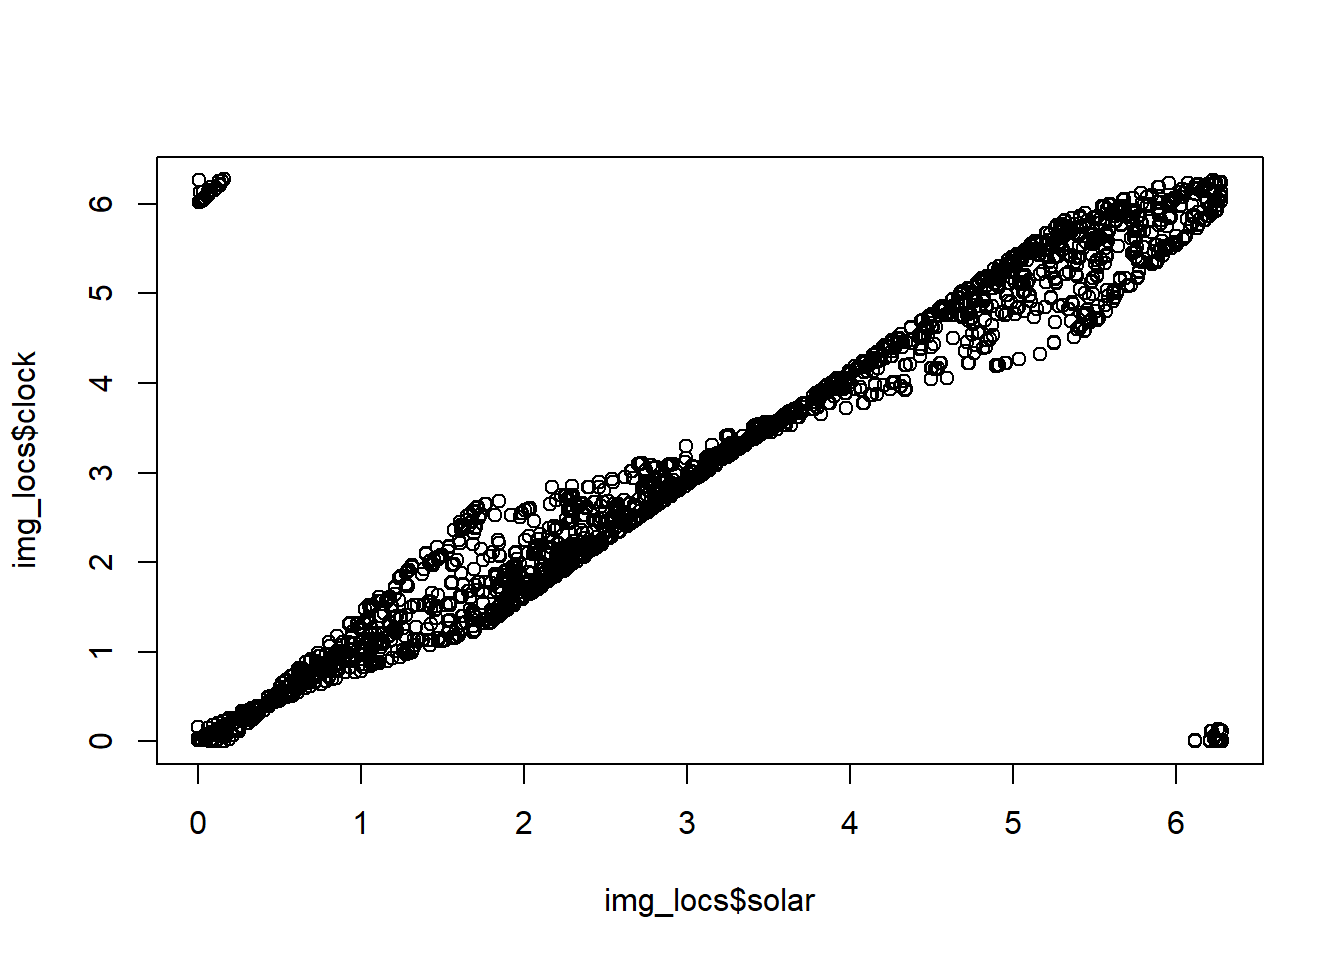
\includegraphics{bookdown-demo_files/figure-latex/unnamed-chunk-46-1.pdf}

\section{Other resources}\label{other-resources}

Palmer, Meredith S., et al. ``Evaluating relative abundance indices for
terrestrial herbivores from large‐scale camera trap surveys.'' African
journal of ecology 56.4 (2018): 791-803.

\chapter{Occupancy}\label{occupancy}

Name a better duo than that camera trapping and occupancy modelling.
I'll wait.

Occupancy modelling has been the mainstay of analysing data from camera
traps since

\textbf{Assumptions}

Ideally camera stations would be indpendent of one another, you would
should only capture a given individual on a single camera. Thus for
single species studies research space cameras by a single ``home range''
- although this in itself is tricky to quantify.

ETC

\section{Single species occupancy
model}\label{single-species-occupancy-model}

In this example we will use the weekly observations dataframe fro the
SingleSiteExploration script.

\begin{Shaded}
\begin{Highlighting}[]
\NormalTok{weekObs <-}\StringTok{ }\KeywordTok{read.csv}\NormalTok{(}\StringTok{"data/processed_data/Algar_30min_Independent_Weekly_observations.csv"}\NormalTok{, }\DataTypeTok{header=}\NormalTok{T)}
\end{Highlighting}
\end{Shaded}

Which, as a quick reminder, looks like this:

\begin{Shaded}
\begin{Highlighting}[]
\KeywordTok{kbl}\NormalTok{(weekObs)}\OperatorTok
\StringTok{  }\KeywordTok{kable_paper}\NormalTok{() }\OperatorTok
\StringTok{  }\KeywordTok{scroll_box}\NormalTok{( }\DataTypeTok{height =} \StringTok{"200px"}\NormalTok{)}
\end{Highlighting}
\end{Shaded}

\begin{table}
\centering
\begin{tabular}[t]{l|l|r|r|r|r|r|r|r|r|r|r|r|r|r}
\hline
Deployment.Location.ID & Date & Effort & Alces.alces & Canis.latrans & Canis.lupus & Cervus.canadensis & Grus.canadensis & Lepus.americanus & Lynx.canadensis & Martes.americana & Odocoileus.virginianus & Rangifer.tarandus & Tamiasciurus.hudsonicus & Ursus.americanus\\
\hline
Algar08 & 2018-W45 & 1 & 0 & 0 & 0 & 0 & 0 & 0 & 0 & 0 & 0 & 0 & 0 & 0\\
\hline
Algar08 & 2018-W46 & 7 & 0 & 0 & 0 & 0 & 0 & 0 & 0 & 0 & 0 & 0 & 0 & 0\\
\hline
Algar08 & 2018-W47 & 7 & 0 & 0 & 0 & 0 & 0 & 0 & 0 & 0 & 0 & 0 & 0 & 0\\
\hline
Algar08 & 2018-W48 & 7 & 0 & 0 & 0 & 0 & 0 & 0 & 0 & 0 & 0 & 0 & 0 & 0\\
\hline
Algar08 & 2018-W49 & 7 & 0 & 0 & 0 & 0 & 0 & 0 & 0 & 0 & 0 & 0 & 0 & 0\\
\hline
Algar08 & 2018-W50 & 7 & 0 & 0 & 0 & 0 & 0 & 0 & 0 & 0 & 1 & 0 & 0 & 0\\
\hline
Algar08 & 2018-W51 & 7 & 0 & 0 & 0 & 0 & 0 & 0 & 0 & 0 & 0 & 0 & 0 & 0\\
\hline
Algar08 & 2018-W52 & 2 & 0 & 0 & 0 & 0 & 0 & 0 & 0 & 0 & 0 & 0 & 0 & 0\\
\hline
Algar08 & 2019-W00 & 5 & 0 & 0 & 0 & 0 & 0 & 0 & 0 & 0 & 0 & 0 & 0 & 0\\
\hline
Algar08 & 2019-W01 & 7 & 0 & 0 & 0 & 0 & 0 & 0 & 0 & 0 & 0 & 0 & 0 & 0\\
\hline
Algar08 & 2019-W02 & 7 & 0 & 0 & 0 & 0 & 0 & 0 & 0 & 0 & 0 & 0 & 0 & 0\\
\hline
Algar08 & 2019-W03 & 7 & 0 & 0 & 0 & 0 & 0 & 0 & 0 & 0 & 0 & 0 & 0 & 0\\
\hline
Algar08 & 2019-W04 & 7 & 0 & 0 & 0 & 0 & 0 & 0 & 0 & 0 & 0 & 0 & 0 & 0\\
\hline
Algar08 & 2019-W05 & 7 & 0 & 0 & 0 & 0 & 0 & 0 & 0 & 0 & 0 & 0 & 0 & 0\\
\hline
Algar08 & 2019-W06 & 7 & 0 & 0 & 0 & 0 & 0 & 0 & 0 & 0 & 0 & 0 & 0 & 0\\
\hline
Algar08 & 2019-W07 & 7 & 0 & 0 & 0 & 0 & 0 & 0 & 0 & 0 & 0 & 0 & 0 & 0\\
\hline
Algar08 & 2019-W08 & 7 & 0 & 0 & 0 & 0 & 0 & 0 & 0 & 0 & 0 & 0 & 0 & 0\\
\hline
Algar08 & 2019-W09 & 7 & 0 & 0 & 0 & 0 & 0 & 0 & 0 & 0 & 0 & 0 & 0 & 0\\
\hline
Algar08 & 2019-W10 & 7 & 0 & 0 & 0 & 0 & 0 & 0 & 0 & 0 & 0 & 0 & 0 & 0\\
\hline
Algar08 & 2019-W11 & 7 & 0 & 0 & 0 & 0 & 0 & 0 & 0 & 0 & 0 & 0 & 0 & 0\\
\hline
Algar08 & 2019-W12 & 7 & 0 & 0 & 0 & 0 & 0 & 0 & 0 & 0 & 0 & 0 & 0 & 0\\
\hline
Algar08 & 2019-W13 & 7 & 0 & 0 & 0 & 0 & 0 & 0 & 0 & 0 & 0 & 0 & 0 & 0\\
\hline
Algar08 & 2019-W14 & 7 & 0 & 0 & 0 & 0 & 0 & 0 & 0 & 0 & 0 & 0 & 0 & 0\\
\hline
Algar08 & 2019-W15 & 7 & 1 & 0 & 0 & 0 & 0 & 0 & 0 & 0 & 0 & 0 & 0 & 0\\
\hline
Algar08 & 2019-W16 & 7 & 1 & 0 & 0 & 0 & 0 & 0 & 0 & 0 & 0 & 0 & 0 & 0\\
\hline
Algar08 & 2019-W17 & 7 & 0 & 0 & 0 & 0 & 0 & 0 & 0 & 0 & 0 & 0 & 0 & 0\\
\hline
Algar08 & 2019-W18 & 7 & 0 & 0 & 0 & 0 & 0 & 0 & 0 & 0 & 1 & 0 & 0 & 0\\
\hline
Algar08 & 2019-W19 & 7 & 0 & 0 & 0 & 0 & 0 & 0 & 0 & 0 & 0 & 0 & 0 & 0\\
\hline
Algar08 & 2019-W20 & 7 & 0 & 0 & 0 & 0 & 0 & 0 & 0 & 0 & 0 & 1 & 0 & 0\\
\hline
Algar08 & 2019-W21 & 7 & 0 & 0 & 0 & 0 & 0 & 0 & 0 & 0 & 0 & 0 & 0 & 0\\
\hline
Algar08 & 2019-W22 & 7 & 0 & 0 & 0 & 0 & 0 & 0 & 0 & 0 & 0 & 0 & 0 & 0\\
\hline
Algar08 & 2019-W23 & 7 & 0 & 0 & 0 & 0 & 0 & 0 & 0 & 0 & 0 & 0 & 0 & 0\\
\hline
Algar08 & 2019-W24 & 7 & 0 & 0 & 0 & 0 & 0 & 0 & 0 & 0 & 0 & 0 & 0 & 0\\
\hline
Algar08 & 2019-W25 & 7 & 0 & 0 & 0 & 0 & 0 & 0 & 0 & 0 & 0 & 0 & 0 & 0\\
\hline
Algar08 & 2019-W26 & 7 & 0 & 0 & 0 & 0 & 0 & 0 & 0 & 0 & 0 & 0 & 0 & 0\\
\hline
Algar08 & 2019-W27 & 7 & 0 & 0 & 0 & 0 & 0 & 0 & 0 & 0 & 0 & 0 & 0 & 0\\
\hline
Algar08 & 2019-W28 & 7 & 0 & 0 & 0 & 0 & 0 & 0 & 0 & 0 & 0 & 0 & 0 & 0\\
\hline
Algar08 & 2019-W29 & 7 & 0 & 0 & 0 & 0 & 0 & 0 & 0 & 0 & 0 & 0 & 0 & 0\\
\hline
Algar08 & 2019-W30 & 7 & 1 & 0 & 0 & 0 & 0 & 0 & 0 & 0 & 0 & 0 & 0 & 0\\
\hline
Algar08 & 2019-W31 & 7 & 0 & 0 & 0 & 0 & 0 & 0 & 0 & 0 & 0 & 0 & 0 & 0\\
\hline
Algar08 & 2019-W32 & 7 & 2 & 0 & 0 & 0 & 0 & 1 & 0 & 0 & 0 & 0 & 0 & 0\\
\hline
Algar08 & 2019-W33 & 7 & 0 & 0 & 0 & 0 & 0 & 0 & 0 & 0 & 0 & 0 & 0 & 0\\
\hline
Algar08 & 2019-W34 & 7 & 0 & 0 & 0 & 0 & 0 & 0 & 0 & 0 & 0 & 0 & 0 & 0\\
\hline
Algar08 & 2019-W35 & 7 & 0 & 0 & 0 & 0 & 0 & 0 & 0 & 0 & 0 & 0 & 0 & 0\\
\hline
Algar08 & 2019-W36 & 7 & 0 & 0 & 0 & 0 & 0 & 0 & 0 & 0 & 0 & 0 & 0 & 0\\
\hline
Algar08 & 2019-W37 & 7 & 0 & 0 & 0 & 0 & 0 & 0 & 0 & 0 & 0 & 0 & 0 & 0\\
\hline
Algar08 & 2019-W38 & 7 & 0 & 0 & 0 & 0 & 0 & 0 & 0 & 0 & 0 & 0 & 0 & 0\\
\hline
Algar08 & 2019-W39 & 7 & 0 & 0 & 0 & 0 & 0 & 0 & 0 & 0 & 0 & 0 & 0 & 0\\
\hline
Algar08 & 2019-W40 & 7 & 0 & 0 & 0 & 0 & 0 & 0 & 0 & 0 & 0 & 0 & 0 & 0\\
\hline
Algar08 & 2019-W41 & 7 & 0 & 0 & 0 & 0 & 0 & 0 & 0 & 0 & 0 & 0 & 0 & 0\\
\hline
Algar08 & 2019-W42 & 7 & 0 & 0 & 0 & 0 & 0 & 0 & 0 & 0 & 0 & 0 & 0 & 0\\
\hline
Algar08 & 2019-W43 & 7 & 0 & 0 & 0 & 0 & 0 & 0 & 0 & 0 & 0 & 0 & 0 & 0\\
\hline
Algar08 & 2019-W44 & 7 & 0 & 0 & 0 & 0 & 0 & 0 & 0 & 0 & 0 & 0 & 0 & 0\\
\hline
Algar08 & 2019-W45 & 7 & 0 & 0 & 0 & 0 & 0 & 0 & 0 & 0 & 0 & 0 & 0 & 0\\
\hline
Algar08 & 2019-W46 & 5 & 0 & 0 & 1 & 0 & 0 & 0 & 0 & 0 & 0 & 0 & 0 & 0\\
\hline
Algar27 & 2018-W45 & 3 & 0 & 0 & 0 & 0 & 0 & 0 & 0 & 0 & 1 & 0 & 0 & 0\\
\hline
Algar27 & 2018-W46 & 7 & 0 & 0 & 0 & 1 & 0 & 0 & 0 & 0 & 0 & 0 & 0 & 0\\
\hline
Algar27 & 2018-W47 & 7 & 0 & 1 & 0 & 0 & 0 & 0 & 0 & 0 & 0 & 0 & 0 & 0\\
\hline
Algar27 & 2018-W48 & 7 & 0 & 0 & 0 & 0 & 0 & 0 & 0 & 0 & 0 & 0 & 0 & 0\\
\hline
Algar27 & 2018-W49 & 7 & 0 & 0 & 2 & 0 & 0 & 0 & 0 & 0 & 0 & 0 & 0 & 0\\
\hline
Algar27 & 2018-W50 & 7 & 0 & 0 & 0 & 0 & 0 & 0 & 0 & 0 & 0 & 0 & 0 & 0\\
\hline
Algar27 & 2018-W51 & 7 & 0 & 0 & 0 & 0 & 0 & 0 & 0 & 0 & 0 & 0 & 0 & 0\\
\hline
Algar27 & 2018-W52 & 2 & 0 & 0 & 0 & 0 & 0 & 0 & 0 & 0 & 0 & 0 & 0 & 0\\
\hline
Algar27 & 2019-W00 & 5 & 0 & 1 & 0 & 0 & 0 & 0 & 0 & 0 & 0 & 0 & 0 & 0\\
\hline
Algar27 & 2019-W01 & 7 & 0 & 1 & 1 & 0 & 0 & 0 & 0 & 0 & 0 & 0 & 0 & 0\\
\hline
Algar27 & 2019-W02 & 7 & 0 & 0 & 0 & 0 & 0 & 0 & 0 & 0 & 0 & 0 & 0 & 0\\
\hline
Algar27 & 2019-W03 & 7 & 0 & 0 & 0 & 0 & 0 & 0 & 0 & 0 & 0 & 0 & 0 & 0\\
\hline
Algar27 & 2019-W04 & 7 & 1 & 0 & 0 & 0 & 0 & 0 & 0 & 0 & 0 & 0 & 0 & 0\\
\hline
Algar27 & 2019-W05 & 7 & 0 & 0 & 0 & 0 & 0 & 0 & 0 & 0 & 0 & 0 & 0 & 0\\
\hline
Algar27 & 2019-W06 & 7 & 0 & 0 & 1 & 0 & 0 & 0 & 0 & 0 & 0 & 0 & 0 & 0\\
\hline
Algar27 & 2019-W07 & 7 & 0 & 0 & 0 & 0 & 0 & 0 & 1 & 0 & 0 & 0 & 0 & 0\\
\hline
Algar27 & 2019-W08 & 7 & 0 & 0 & 0 & 0 & 0 & 0 & 0 & 0 & 0 & 0 & 0 & 0\\
\hline
Algar27 & 2019-W09 & 7 & 0 & 0 & 0 & 0 & 0 & 0 & 0 & 0 & 0 & 0 & 0 & 0\\
\hline
Algar27 & 2019-W10 & 7 & 0 & 0 & 0 & 0 & 0 & 0 & 0 & 0 & 0 & 0 & 0 & 0\\
\hline
Algar27 & 2019-W11 & 7 & 0 & 0 & 0 & 0 & 0 & 0 & 2 & 0 & 0 & 0 & 0 & 0\\
\hline
Algar27 & 2019-W12 & 7 & 0 & 0 & 0 & 0 & 0 & 0 & 1 & 0 & 0 & 0 & 0 & 0\\
\hline
Algar27 & 2019-W13 & 4 & 0 & 0 & 0 & 0 & 0 & 0 & 0 & 0 & 0 & 0 & 0 & 0\\
\hline
Algar29 & 2018-W45 & 3 & 0 & 0 & 0 & 0 & 0 & 0 & 0 & 0 & 0 & 0 & 0 & 0\\
\hline
Algar29 & 2018-W46 & 7 & 0 & 0 & 0 & 0 & 0 & 0 & 0 & 0 & 2 & 0 & 0 & 0\\
\hline
Algar29 & 2018-W47 & 7 & 0 & 0 & 0 & 0 & 0 & 0 & 0 & 0 & 1 & 0 & 0 & 0\\
\hline
Algar29 & 2018-W48 & 7 & 0 & 0 & 0 & 0 & 0 & 0 & 1 & 0 & 1 & 0 & 0 & 0\\
\hline
Algar29 & 2018-W49 & 7 & 0 & 0 & 1 & 0 & 0 & 0 & 0 & 0 & 0 & 0 & 0 & 0\\
\hline
Algar29 & 2018-W50 & 7 & 0 & 0 & 0 & 0 & 0 & 0 & 0 & 0 & 1 & 0 & 0 & 0\\
\hline
Algar29 & 2018-W51 & 7 & 0 & 0 & 0 & 0 & 0 & 0 & 0 & 0 & 0 & 0 & 0 & 0\\
\hline
Algar29 & 2018-W52 & 2 & 0 & 0 & 0 & 0 & 0 & 0 & 0 & 0 & 0 & 0 & 0 & 0\\
\hline
Algar29 & 2019-W00 & 5 & 0 & 0 & 0 & 0 & 0 & 0 & 0 & 0 & 0 & 0 & 0 & 0\\
\hline
Algar29 & 2019-W01 & 7 & 0 & 0 & 0 & 0 & 0 & 0 & 0 & 0 & 0 & 0 & 0 & 0\\
\hline
Algar29 & 2019-W02 & 7 & 0 & 0 & 0 & 0 & 0 & 0 & 0 & 0 & 0 & 0 & 0 & 0\\
\hline
Algar29 & 2019-W03 & 7 & 0 & 0 & 0 & 0 & 0 & 0 & 0 & 0 & 0 & 0 & 0 & 0\\
\hline
Algar29 & 2019-W04 & 7 & 0 & 0 & 0 & 0 & 0 & 0 & 0 & 0 & 0 & 0 & 0 & 0\\
\hline
Algar29 & 2019-W05 & 7 & 0 & 0 & 0 & 0 & 0 & 0 & 0 & 0 & 0 & 0 & 0 & 0\\
\hline
Algar29 & 2019-W06 & 7 & 1 & 0 & 0 & 0 & 0 & 0 & 0 & 0 & 0 & 0 & 0 & 0\\
\hline
Algar29 & 2019-W07 & 7 & 0 & 0 & 0 & 0 & 0 & 0 & 0 & 0 & 0 & 0 & 0 & 0\\
\hline
Algar29 & 2019-W08 & 7 & 0 & 0 & 0 & 0 & 0 & 0 & 0 & 0 & 0 & 0 & 0 & 0\\
\hline
Algar29 & 2019-W09 & 7 & 0 & 0 & 0 & 0 & 0 & 0 & 0 & 0 & 0 & 0 & 0 & 0\\
\hline
Algar29 & 2019-W10 & 7 & 0 & 0 & 0 & 0 & 0 & 0 & 0 & 0 & 0 & 0 & 0 & 0\\
\hline
Algar29 & 2019-W11 & 7 & 0 & 0 & 0 & 0 & 0 & 0 & 0 & 0 & 0 & 0 & 0 & 0\\
\hline
Algar29 & 2019-W12 & 7 & 0 & 0 & 0 & 0 & 0 & 0 & 0 & 0 & 0 & 0 & 0 & 0\\
\hline
Algar29 & 2019-W13 & 7 & 0 & 0 & 0 & 0 & 0 & 0 & 0 & 0 & 0 & 0 & 0 & 0\\
\hline
Algar29 & 2019-W14 & 7 & 0 & 0 & 0 & 0 & 0 & 0 & 0 & 0 & 2 & 0 & 0 & 0\\
\hline
Algar29 & 2019-W15 & 7 & 1 & 0 & 0 & 0 & 0 & 0 & 0 & 0 & 0 & 0 & 0 & 1\\
\hline
Algar29 & 2019-W16 & 7 & 1 & 0 & 0 & 0 & 0 & 0 & 0 & 0 & 1 & 0 & 0 & 0\\
\hline
Algar29 & 2019-W17 & 7 & 0 & 0 & 0 & 0 & 3 & 0 & 0 & 0 & 0 & 0 & 0 & 0\\
\hline
Algar29 & 2019-W18 & 7 & 0 & 0 & 0 & 0 & 2 & 0 & 0 & 0 & 1 & 0 & 0 & 0\\
\hline
Algar29 & 2019-W19 & 7 & 1 & 0 & 0 & 0 & 0 & 0 & 0 & 0 & 1 & 0 & 0 & 0\\
\hline
Algar29 & 2019-W20 & 7 & 0 & 0 & 0 & 0 & 2 & 0 & 0 & 0 & 4 & 0 & 0 & 0\\
\hline
Algar29 & 2019-W21 & 7 & 1 & 0 & 0 & 0 & 2 & 0 & 0 & 0 & 0 & 0 & 0 & 0\\
\hline
Algar29 & 2019-W22 & 7 & 1 & 0 & 0 & 0 & 0 & 0 & 0 & 0 & 0 & 0 & 0 & 2\\
\hline
Algar29 & 2019-W23 & 7 & 1 & 0 & 0 & 0 & 0 & 0 & 0 & 0 & 0 & 0 & 0 & 0\\
\hline
Algar29 & 2019-W24 & 7 & 0 & 0 & 0 & 0 & 0 & 0 & 0 & 0 & 0 & 0 & 0 & 0\\
\hline
Algar29 & 2019-W25 & 7 & 0 & 0 & 0 & 0 & 0 & 0 & 0 & 0 & 1 & 0 & 0 & 0\\
\hline
Algar29 & 2019-W26 & 7 & 0 & 0 & 0 & 0 & 1 & 0 & 0 & 0 & 0 & 0 & 0 & 0\\
\hline
Algar29 & 2019-W27 & 7 & 0 & 0 & 0 & 0 & 0 & 0 & 0 & 0 & 0 & 0 & 0 & 0\\
\hline
Algar29 & 2019-W28 & 7 & 0 & 0 & 0 & 0 & 0 & 0 & 0 & 0 & 0 & 0 & 0 & 0\\
\hline
Algar29 & 2019-W29 & 7 & 0 & 0 & 0 & 0 & 0 & 0 & 0 & 0 & 0 & 0 & 0 & 0\\
\hline
Algar29 & 2019-W30 & 7 & 0 & 0 & 0 & 0 & 2 & 0 & 0 & 0 & 0 & 0 & 0 & 0\\
\hline
Algar29 & 2019-W31 & 7 & 0 & 0 & 0 & 0 & 1 & 0 & 0 & 0 & 0 & 0 & 0 & 1\\
\hline
Algar29 & 2019-W32 & 7 & 0 & 0 & 0 & 0 & 0 & 0 & 0 & 0 & 0 & 0 & 0 & 0\\
\hline
Algar29 & 2019-W33 & 7 & 0 & 0 & 0 & 0 & 0 & 0 & 0 & 0 & 2 & 0 & 0 & 0\\
\hline
Algar29 & 2019-W34 & 7 & 0 & 0 & 0 & 0 & 0 & 0 & 0 & 0 & 0 & 0 & 0 & 0\\
\hline
Algar29 & 2019-W35 & 7 & 0 & 0 & 0 & 0 & 0 & 0 & 0 & 0 & 0 & 0 & 0 & 0\\
\hline
Algar29 & 2019-W36 & 7 & 0 & 0 & 0 & 0 & 0 & 0 & 0 & 0 & 1 & 0 & 0 & 0\\
\hline
Algar29 & 2019-W37 & 7 & 0 & 0 & 0 & 0 & 0 & 0 & 0 & 0 & 0 & 0 & 0 & 0\\
\hline
Algar29 & 2019-W38 & 7 & 0 & 0 & 0 & 0 & 0 & 0 & 0 & 0 & 0 & 0 & 0 & 2\\
\hline
Algar29 & 2019-W39 & 7 & 0 & 0 & 0 & 0 & 0 & 0 & 0 & 0 & 0 & 0 & 0 & 1\\
\hline
Algar29 & 2019-W40 & 7 & 0 & 0 & 0 & 0 & 0 & 0 & 0 & 0 & 0 & 0 & 0 & 0\\
\hline
Algar29 & 2019-W41 & 7 & 0 & 0 & 0 & 0 & 0 & 0 & 0 & 0 & 0 & 0 & 0 & 0\\
\hline
Algar29 & 2019-W42 & 7 & 0 & 0 & 0 & 0 & 0 & 0 & 0 & 0 & 1 & 0 & 0 & 0\\
\hline
Algar29 & 2019-W43 & 7 & 0 & 0 & 0 & 0 & 0 & 0 & 0 & 0 & 3 & 0 & 0 & 0\\
\hline
Algar29 & 2019-W44 & 7 & 0 & 0 & 0 & 0 & 0 & 0 & 0 & 0 & 1 & 0 & 0 & 0\\
\hline
Algar29 & 2019-W45 & 7 & 0 & 0 & 0 & 0 & 0 & 0 & 0 & 0 & 1 & 0 & 0 & 0\\
\hline
Algar29 & 2019-W46 & 4 & 0 & 0 & 0 & 0 & 0 & 0 & 0 & 0 & 0 & 0 & 0 & 0\\
\hline
Algar31 & 2018-W45 & 2 & 0 & 0 & 0 & 0 & 0 & 0 & 0 & 0 & 0 & 0 & 0 & 0\\
\hline
Algar31 & 2018-W46 & 7 & 0 & 0 & 0 & 0 & 0 & 0 & 0 & 0 & 0 & 0 & 0 & 0\\
\hline
Algar31 & 2018-W47 & 7 & 0 & 0 & 0 & 0 & 0 & 0 & 0 & 0 & 0 & 0 & 0 & 0\\
\hline
Algar31 & 2018-W48 & 7 & 0 & 0 & 0 & 0 & 0 & 0 & 0 & 0 & 0 & 0 & 0 & 0\\
\hline
Algar31 & 2018-W49 & 7 & 0 & 0 & 0 & 0 & 0 & 0 & 0 & 0 & 0 & 0 & 0 & 0\\
\hline
Algar31 & 2018-W50 & 7 & 0 & 0 & 0 & 0 & 0 & 0 & 0 & 0 & 0 & 0 & 0 & 0\\
\hline
Algar31 & 2018-W51 & 7 & 1 & 0 & 0 & 0 & 0 & 0 & 0 & 0 & 0 & 0 & 0 & 0\\
\hline
Algar31 & 2018-W52 & 2 & 0 & 0 & 0 & 0 & 0 & 0 & 0 & 0 & 0 & 0 & 0 & 0\\
\hline
Algar31 & 2019-W00 & 5 & 0 & 0 & 0 & 0 & 0 & 0 & 0 & 0 & 0 & 0 & 0 & 0\\
\hline
Algar31 & 2019-W01 & 7 & 0 & 0 & 0 & 0 & 0 & 0 & 0 & 0 & 0 & 0 & 0 & 0\\
\hline
Algar31 & 2019-W02 & 7 & 0 & 0 & 0 & 0 & 0 & 0 & 0 & 0 & 0 & 0 & 0 & 0\\
\hline
Algar31 & 2019-W03 & 7 & 0 & 0 & 0 & 0 & 0 & 0 & 0 & 0 & 0 & 0 & 0 & 0\\
\hline
Algar31 & 2019-W04 & 7 & 0 & 0 & 0 & 0 & 0 & 0 & 0 & 0 & 0 & 0 & 0 & 0\\
\hline
Algar31 & 2019-W05 & 7 & 0 & 0 & 0 & 0 & 0 & 0 & 0 & 0 & 0 & 0 & 0 & 0\\
\hline
Algar31 & 2019-W06 & 7 & 0 & 0 & 0 & 0 & 0 & 0 & 0 & 0 & 0 & 0 & 0 & 0\\
\hline
Algar31 & 2019-W07 & 7 & 0 & 0 & 0 & 0 & 0 & 0 & 0 & 0 & 0 & 0 & 0 & 0\\
\hline
Algar31 & 2019-W08 & 7 & 0 & 0 & 0 & 0 & 0 & 0 & 0 & 0 & 0 & 0 & 0 & 0\\
\hline
Algar31 & 2019-W09 & 7 & 0 & 0 & 0 & 0 & 0 & 0 & 0 & 0 & 0 & 0 & 0 & 0\\
\hline
Algar31 & 2019-W10 & 7 & 0 & 0 & 0 & 0 & 0 & 0 & 0 & 0 & 0 & 0 & 0 & 0\\
\hline
Algar31 & 2019-W11 & 7 & 0 & 0 & 0 & 0 & 0 & 0 & 0 & 2 & 0 & 0 & 0 & 0\\
\hline
Algar31 & 2019-W12 & 7 & 0 & 0 & 0 & 0 & 0 & 0 & 0 & 0 & 0 & 0 & 0 & 0\\
\hline
Algar31 & 2019-W13 & 7 & 1 & 0 & 2 & 0 & 0 & 0 & 0 & 0 & 0 & 0 & 0 & 0\\
\hline
Algar31 & 2019-W14 & 7 & 0 & 0 & 0 & 0 & 0 & 0 & 0 & 0 & 0 & 0 & 0 & 0\\
\hline
Algar31 & 2019-W15 & 7 & 0 & 0 & 1 & 0 & 0 & 0 & 0 & 0 & 0 & 0 & 0 & 0\\
\hline
Algar31 & 2019-W16 & 7 & 0 & 0 & 1 & 0 & 1 & 0 & 0 & 0 & 0 & 0 & 0 & 0\\
\hline
Algar31 & 2019-W17 & 7 & 0 & 0 & 1 & 0 & 0 & 0 & 0 & 0 & 0 & 0 & 0 & 0\\
\hline
Algar31 & 2019-W18 & 7 & 0 & 0 & 0 & 0 & 3 & 0 & 0 & 0 & 0 & 0 & 0 & 0\\
\hline
Algar31 & 2019-W19 & 7 & 0 & 0 & 0 & 0 & 0 & 0 & 0 & 0 & 0 & 0 & 0 & 0\\
\hline
Algar31 & 2019-W20 & 7 & 0 & 0 & 0 & 0 & 0 & 0 & 0 & 0 & 0 & 0 & 0 & 0\\
\hline
Algar31 & 2019-W21 & 7 & 0 & 0 & 0 & 0 & 0 & 0 & 0 & 1 & 0 & 0 & 0 & 0\\
\hline
Algar31 & 2019-W22 & 7 & 0 & 0 & 0 & 0 & 2 & 0 & 0 & 0 & 0 & 0 & 0 & 0\\
\hline
Algar31 & 2019-W23 & 7 & 1 & 0 & 0 & 0 & 1 & 0 & 0 & 0 & 1 & 1 & 0 & 0\\
\hline
Algar31 & 2019-W24 & 7 & 0 & 0 & 1 & 0 & 1 & 0 & 0 & 0 & 0 & 1 & 0 & 0\\
\hline
Algar31 & 2019-W25 & 7 & 0 & 0 & 0 & 0 & 0 & 0 & 0 & 0 & 0 & 1 & 0 & 0\\
\hline
Algar31 & 2019-W26 & 7 & 0 & 0 & 0 & 0 & 0 & 0 & 0 & 0 & 0 & 1 & 0 & 0\\
\hline
Algar31 & 2019-W27 & 7 & 0 & 0 & 0 & 0 & 0 & 0 & 0 & 0 & 0 & 0 & 0 & 0\\
\hline
Algar31 & 2019-W28 & 7 & 0 & 0 & 0 & 0 & 1 & 0 & 0 & 0 & 0 & 1 & 0 & 0\\
\hline
Algar31 & 2019-W29 & 7 & 0 & 0 & 0 & 0 & 0 & 0 & 0 & 0 & 0 & 0 & 0 & 1\\
\hline
Algar31 & 2019-W30 & 7 & 0 & 0 & 0 & 0 & 2 & 0 & 0 & 0 & 0 & 1 & 0 & 0\\
\hline
Algar31 & 2019-W31 & 7 & 0 & 0 & 0 & 0 & 0 & 0 & 0 & 0 & 0 & 0 & 0 & 0\\
\hline
Algar31 & 2019-W32 & 7 & 0 & 0 & 0 & 0 & 1 & 0 & 0 & 0 & 0 & 0 & 0 & 0\\
\hline
Algar31 & 2019-W33 & 7 & 0 & 0 & 0 & 0 & 1 & 0 & 0 & 0 & 0 & 0 & 0 & 0\\
\hline
Algar31 & 2019-W34 & 7 & 0 & 0 & 0 & 0 & 0 & 0 & 0 & 0 & 0 & 0 & 0 & 0\\
\hline
Algar31 & 2019-W35 & 7 & 0 & 0 & 0 & 0 & 0 & 0 & 0 & 0 & 0 & 0 & 0 & 0\\
\hline
Algar31 & 2019-W36 & 7 & 0 & 0 & 0 & 0 & 0 & 0 & 0 & 0 & 0 & 2 & 0 & 0\\
\hline
Algar31 & 2019-W37 & 7 & 0 & 0 & 0 & 0 & 0 & 0 & 0 & 0 & 0 & 3 & 0 & 0\\
\hline
Algar31 & 2019-W38 & 7 & 0 & 0 & 0 & 0 & 0 & 0 & 0 & 0 & 0 & 3 & 0 & 0\\
\hline
Algar31 & 2019-W39 & 7 & 0 & 0 & 0 & 0 & 0 & 0 & 0 & 0 & 0 & 0 & 0 & 0\\
\hline
Algar31 & 2019-W40 & 7 & 0 & 0 & 0 & 0 & 0 & 0 & 0 & 0 & 0 & 0 & 0 & 0\\
\hline
Algar31 & 2019-W41 & 7 & 0 & 0 & 0 & 0 & 0 & 0 & 0 & 0 & 0 & 1 & 0 & 1\\
\hline
Algar31 & 2019-W42 & 7 & 0 & 0 & 0 & 0 & 0 & 0 & 0 & 0 & 0 & 0 & 0 & 0\\
\hline
Algar31 & 2019-W43 & 7 & 0 & 0 & 0 & 0 & 0 & 0 & 0 & 0 & 0 & 0 & 0 & 0\\
\hline
Algar31 & 2019-W44 & 7 & 0 & 0 & 0 & 0 & 0 & 0 & 0 & 0 & 0 & 0 & 0 & 0\\
\hline
Algar31 & 2019-W45 & 7 & 0 & 0 & 0 & 0 & 0 & 0 & 0 & 0 & 0 & 0 & 0 & 0\\
\hline
Algar31 & 2019-W46 & 5 & 0 & 0 & 0 & 0 & 0 & 1 & 0 & 1 & 0 & 0 & 0 & 0\\
\hline
Algar32 & 2018-W45 & 4 & 0 & 0 & 0 & 0 & 0 & 0 & 0 & 0 & 0 & 0 & 0 & 0\\
\hline
Algar32 & 2018-W46 & 7 & 1 & 0 & 0 & 0 & 0 & 0 & 0 & 0 & 0 & 0 & 0 & 0\\
\hline
Algar32 & 2018-W47 & 7 & 0 & 0 & 0 & 0 & 0 & 0 & 0 & 0 & 0 & 0 & 0 & 0\\
\hline
Algar32 & 2018-W48 & 7 & 0 & 0 & 0 & 0 & 0 & 0 & 0 & 0 & 0 & 0 & 0 & 0\\
\hline
Algar32 & 2018-W49 & 7 & 0 & 0 & 0 & 0 & 0 & 0 & 0 & 0 & 0 & 0 & 0 & 0\\
\hline
Algar32 & 2018-W50 & 7 & 0 & 0 & 0 & 0 & 0 & 0 & 0 & 0 & 0 & 0 & 0 & 0\\
\hline
Algar32 & 2018-W51 & 7 & 0 & 0 & 0 & 0 & 0 & 0 & 0 & 0 & 0 & 0 & 0 & 0\\
\hline
Algar32 & 2018-W52 & 2 & 0 & 0 & 0 & 0 & 0 & 0 & 0 & 0 & 0 & 0 & 0 & 0\\
\hline
Algar32 & 2019-W00 & 5 & 0 & 0 & 0 & 0 & 0 & 0 & 0 & 0 & 0 & 0 & 0 & 0\\
\hline
Algar32 & 2019-W01 & 7 & 0 & 0 & 0 & 0 & 0 & 0 & 0 & 0 & 0 & 0 & 0 & 0\\
\hline
Algar32 & 2019-W02 & 7 & 0 & 0 & 0 & 0 & 0 & 0 & 0 & 0 & 0 & 0 & 0 & 0\\
\hline
Algar32 & 2019-W03 & 7 & 0 & 0 & 0 & 0 & 0 & 0 & 0 & 0 & 0 & 0 & 0 & 0\\
\hline
Algar32 & 2019-W04 & 7 & 0 & 0 & 0 & 0 & 0 & 0 & 0 & 0 & 0 & 0 & 0 & 0\\
\hline
Algar32 & 2019-W05 & 7 & 0 & 0 & 0 & 0 & 0 & 0 & 0 & 0 & 0 & 0 & 0 & 0\\
\hline
Algar32 & 2019-W06 & 7 & 0 & 0 & 0 & 0 & 0 & 0 & 0 & 0 & 0 & 0 & 0 & 0\\
\hline
Algar32 & 2019-W07 & 7 & 0 & 0 & 0 & 0 & 0 & 0 & 0 & 0 & 0 & 0 & 0 & 0\\
\hline
Algar32 & 2019-W08 & 7 & 0 & 0 & 0 & 0 & 0 & 0 & 0 & 0 & 0 & 0 & 0 & 0\\
\hline
Algar32 & 2019-W09 & 7 & 0 & 0 & 0 & 0 & 0 & 0 & 0 & 0 & 0 & 0 & 0 & 0\\
\hline
Algar32 & 2019-W10 & 7 & 0 & 0 & 0 & 0 & 0 & 0 & 0 & 0 & 0 & 0 & 0 & 0\\
\hline
Algar32 & 2019-W11 & 7 & 0 & 0 & 0 & 0 & 0 & 0 & 0 & 0 & 0 & 0 & 0 & 0\\
\hline
Algar32 & 2019-W12 & 7 & 0 & 0 & 0 & 0 & 0 & 0 & 0 & 0 & 0 & 0 & 0 & 0\\
\hline
Algar32 & 2019-W13 & 7 & 0 & 0 & 0 & 0 & 0 & 0 & 0 & 0 & 0 & 0 & 0 & 0\\
\hline
Algar32 & 2019-W14 & 7 & 0 & 0 & 0 & 0 & 0 & 0 & 0 & 0 & 0 & 0 & 0 & 0\\
\hline
Algar32 & 2019-W15 & 7 & 0 & 0 & 0 & 0 & 0 & 0 & 0 & 0 & 0 & 0 & 0 & 0\\
\hline
Algar32 & 2019-W16 & 7 & 0 & 0 & 0 & 0 & 0 & 0 & 0 & 0 & 0 & 0 & 0 & 0\\
\hline
Algar32 & 2019-W17 & 7 & 0 & 0 & 0 & 0 & 1 & 0 & 0 & 0 & 0 & 0 & 0 & 0\\
\hline
Algar32 & 2019-W18 & 7 & 0 & 0 & 0 & 0 & 0 & 0 & 0 & 0 & 0 & 0 & 0 & 0\\
\hline
Algar32 & 2019-W19 & 7 & 0 & 0 & 0 & 0 & 0 & 0 & 0 & 0 & 0 & 0 & 0 & 0\\
\hline
Algar32 & 2019-W20 & 7 & 0 & 0 & 0 & 0 & 0 & 0 & 0 & 0 & 0 & 0 & 0 & 0\\
\hline
Algar32 & 2019-W21 & 7 & 0 & 0 & 0 & 0 & 0 & 0 & 0 & 0 & 0 & 0 & 0 & 0\\
\hline
Algar32 & 2019-W22 & 7 & 0 & 0 & 0 & 0 & 0 & 0 & 0 & 0 & 0 & 0 & 0 & 0\\
\hline
Algar32 & 2019-W23 & 7 & 0 & 0 & 0 & 0 & 2 & 0 & 0 & 0 & 0 & 0 & 0 & 0\\
\hline
Algar32 & 2019-W24 & 7 & 0 & 0 & 0 & 0 & 0 & 0 & 0 & 0 & 1 & 0 & 0 & 0\\
\hline
Algar32 & 2019-W25 & 7 & 0 & 0 & 0 & 0 & 0 & 0 & 0 & 0 & 0 & 0 & 0 & 0\\
\hline
Algar32 & 2019-W26 & 7 & 0 & 0 & 0 & 0 & 0 & 0 & 0 & 0 & 0 & 0 & 0 & 0\\
\hline
Algar32 & 2019-W27 & 7 & 0 & 0 & 0 & 0 & 0 & 0 & 0 & 0 & 0 & 0 & 0 & 0\\
\hline
Algar32 & 2019-W28 & 7 & 0 & 0 & 0 & 0 & 0 & 0 & 0 & 0 & 0 & 0 & 0 & 0\\
\hline
Algar32 & 2019-W29 & 7 & 0 & 0 & 0 & 0 & 0 & 0 & 0 & 0 & 0 & 1 & 0 & 0\\
\hline
Algar32 & 2019-W30 & 7 & 0 & 0 & 0 & 0 & 0 & 0 & 0 & 0 & 0 & 0 & 0 & 0\\
\hline
Algar32 & 2019-W31 & 7 & 0 & 0 & 0 & 0 & 0 & 0 & 0 & 0 & 0 & 0 & 0 & 0\\
\hline
Algar32 & 2019-W32 & 7 & 0 & 0 & 0 & 0 & 0 & 0 & 0 & 0 & 0 & 0 & 0 & 0\\
\hline
Algar32 & 2019-W33 & 7 & 0 & 0 & 0 & 0 & 0 & 0 & 0 & 0 & 0 & 0 & 0 & 0\\
\hline
Algar32 & 2019-W34 & 7 & 0 & 0 & 0 & 0 & 0 & 0 & 0 & 0 & 0 & 0 & 0 & 0\\
\hline
Algar32 & 2019-W35 & 7 & 0 & 0 & 0 & 0 & 0 & 0 & 0 & 0 & 0 & 0 & 0 & 0\\
\hline
Algar32 & 2019-W36 & 7 & 0 & 0 & 0 & 0 & 0 & 0 & 0 & 0 & 0 & 1 & 0 & 0\\
\hline
Algar32 & 2019-W37 & 7 & 0 & 0 & 0 & 0 & 0 & 0 & 0 & 0 & 0 & 0 & 0 & 0\\
\hline
Algar32 & 2019-W38 & 7 & 0 & 0 & 0 & 0 & 0 & 0 & 0 & 0 & 0 & 0 & 0 & 0\\
\hline
Algar32 & 2019-W39 & 7 & 0 & 0 & 0 & 0 & 0 & 0 & 0 & 0 & 0 & 0 & 0 & 0\\
\hline
Algar32 & 2019-W40 & 7 & 0 & 0 & 0 & 0 & 0 & 0 & 0 & 0 & 0 & 0 & 0 & 0\\
\hline
Algar32 & 2019-W41 & 7 & 0 & 0 & 0 & 0 & 0 & 0 & 0 & 0 & 0 & 0 & 0 & 0\\
\hline
Algar32 & 2019-W42 & 7 & 0 & 0 & 0 & 0 & 0 & 0 & 0 & 0 & 0 & 0 & 0 & 0\\
\hline
Algar32 & 2019-W43 & 7 & 0 & 0 & 0 & 0 & 0 & 0 & 1 & 0 & 0 & 0 & 0 & 0\\
\hline
Algar32 & 2019-W44 & 7 & 0 & 0 & 0 & 0 & 0 & 0 & 0 & 0 & 0 & 0 & 0 & 0\\
\hline
Algar32 & 2019-W45 & 7 & 0 & 0 & 0 & 0 & 0 & 0 & 0 & 0 & 0 & 0 & 0 & 0\\
\hline
Algar32 & 2019-W46 & 3 & 0 & 0 & 0 & 0 & 0 & 0 & 0 & 0 & 0 & 0 & 0 & 0\\
\hline
Algar34 & 2018-W45 & 1 & 0 & 0 & 0 & 0 & 0 & 0 & 0 & 0 & 0 & 0 & 0 & 0\\
\hline
Algar34 & 2018-W46 & 7 & 0 & 0 & 0 & 0 & 0 & 0 & 0 & 0 & 0 & 0 & 0 & 0\\
\hline
Algar34 & 2018-W47 & 7 & 0 & 0 & 0 & 0 & 0 & 0 & 0 & 0 & 1 & 0 & 0 & 0\\
\hline
Algar34 & 2018-W48 & 7 & 0 & 0 & 0 & 0 & 0 & 0 & 0 & 0 & 0 & 0 & 0 & 0\\
\hline
Algar34 & 2018-W49 & 7 & 0 & 0 & 0 & 0 & 0 & 0 & 0 & 0 & 0 & 0 & 0 & 0\\
\hline
Algar34 & 2018-W50 & 7 & 0 & 0 & 0 & 0 & 0 & 0 & 0 & 0 & 0 & 0 & 0 & 0\\
\hline
Algar34 & 2018-W51 & 7 & 0 & 0 & 0 & 0 & 0 & 0 & 0 & 0 & 0 & 0 & 0 & 0\\
\hline
Algar34 & 2018-W52 & 2 & 0 & 0 & 0 & 0 & 0 & 0 & 0 & 0 & 0 & 0 & 0 & 0\\
\hline
Algar34 & 2019-W00 & 5 & 0 & 0 & 0 & 0 & 0 & 0 & 0 & 0 & 0 & 0 & 0 & 0\\
\hline
Algar34 & 2019-W01 & 7 & 0 & 0 & 0 & 0 & 0 & 0 & 1 & 0 & 0 & 0 & 0 & 0\\
\hline
Algar34 & 2019-W02 & 7 & 0 & 0 & 0 & 0 & 0 & 0 & 0 & 0 & 2 & 0 & 0 & 0\\
\hline
Algar34 & 2019-W03 & 7 & 0 & 0 & 0 & 0 & 0 & 0 & 1 & 0 & 0 & 0 & 0 & 0\\
\hline
Algar34 & 2019-W04 & 7 & 0 & 0 & 0 & 0 & 0 & 0 & 0 & 0 & 0 & 0 & 0 & 0\\
\hline
Algar34 & 2019-W05 & 7 & 0 & 0 & 0 & 0 & 0 & 0 & 0 & 0 & 0 & 0 & 0 & 0\\
\hline
Algar34 & 2019-W06 & 7 & 0 & 0 & 0 & 0 & 0 & 0 & 1 & 0 & 0 & 0 & 0 & 0\\
\hline
Algar34 & 2019-W07 & 7 & 0 & 0 & 0 & 0 & 0 & 0 & 0 & 0 & 0 & 0 & 0 & 0\\
\hline
Algar34 & 2019-W08 & 7 & 0 & 0 & 0 & 0 & 0 & 0 & 0 & 0 & 0 & 0 & 0 & 0\\
\hline
Algar34 & 2019-W09 & 7 & 1 & 0 & 0 & 0 & 0 & 0 & 0 & 0 & 0 & 0 & 0 & 0\\
\hline
Algar34 & 2019-W10 & 7 & 0 & 0 & 0 & 0 & 0 & 0 & 0 & 0 & 0 & 0 & 0 & 0\\
\hline
Algar34 & 2019-W11 & 7 & 0 & 0 & 0 & 0 & 0 & 0 & 0 & 0 & 0 & 0 & 0 & 0\\
\hline
Algar34 & 2019-W12 & 7 & 0 & 0 & 0 & 0 & 0 & 0 & 1 & 0 & 0 & 0 & 0 & 0\\
\hline
Algar34 & 2019-W13 & 7 & 0 & 0 & 0 & 0 & 0 & 0 & 0 & 0 & 0 & 0 & 0 & 0\\
\hline
Algar34 & 2019-W14 & 7 & 0 & 0 & 0 & 0 & 0 & 0 & 0 & 0 & 0 & 0 & 0 & 0\\
\hline
Algar34 & 2019-W15 & 7 & 0 & 0 & 0 & 0 & 0 & 0 & 0 & 0 & 0 & 0 & 0 & 0\\
\hline
Algar34 & 2019-W16 & 7 & 0 & 0 & 0 & 0 & 0 & 0 & 0 & 0 & 0 & 0 & 0 & 0\\
\hline
Algar34 & 2019-W17 & 7 & 0 & 0 & 0 & 0 & 0 & 0 & 0 & 0 & 0 & 0 & 0 & 0\\
\hline
Algar34 & 2019-W18 & 7 & 0 & 0 & 0 & 0 & 0 & 0 & 0 & 0 & 0 & 0 & 0 & 0\\
\hline
Algar34 & 2019-W19 & 7 & 0 & 0 & 0 & 0 & 0 & 0 & 0 & 0 & 0 & 0 & 0 & 0\\
\hline
Algar34 & 2019-W20 & 7 & 0 & 0 & 0 & 0 & 0 & 0 & 0 & 0 & 0 & 0 & 0 & 0\\
\hline
Algar34 & 2019-W21 & 7 & 0 & 0 & 0 & 0 & 0 & 0 & 0 & 0 & 0 & 0 & 0 & 0\\
\hline
Algar34 & 2019-W22 & 7 & 0 & 0 & 0 & 0 & 0 & 0 & 0 & 0 & 0 & 0 & 0 & 0\\
\hline
Algar34 & 2019-W23 & 7 & 0 & 0 & 0 & 0 & 0 & 0 & 0 & 0 & 0 & 0 & 0 & 0\\
\hline
Algar34 & 2019-W24 & 7 & 0 & 0 & 0 & 0 & 0 & 0 & 0 & 0 & 0 & 0 & 0 & 0\\
\hline
Algar34 & 2019-W25 & 7 & 0 & 0 & 0 & 0 & 0 & 0 & 0 & 0 & 0 & 0 & 0 & 0\\
\hline
Algar34 & 2019-W26 & 7 & 0 & 0 & 0 & 0 & 0 & 0 & 0 & 0 & 0 & 0 & 0 & 0\\
\hline
Algar34 & 2019-W27 & 7 & 0 & 0 & 0 & 0 & 0 & 0 & 0 & 0 & 0 & 0 & 0 & 0\\
\hline
Algar34 & 2019-W28 & 7 & 0 & 0 & 0 & 0 & 0 & 0 & 0 & 0 & 0 & 0 & 0 & 0\\
\hline
Algar34 & 2019-W29 & 7 & 0 & 0 & 0 & 0 & 0 & 0 & 0 & 0 & 0 & 0 & 0 & 0\\
\hline
Algar34 & 2019-W30 & 7 & 0 & 0 & 0 & 0 & 0 & 0 & 0 & 0 & 0 & 0 & 0 & 0\\
\hline
Algar34 & 2019-W31 & 7 & 0 & 0 & 0 & 0 & 0 & 0 & 0 & 0 & 0 & 0 & 0 & 0\\
\hline
Algar34 & 2019-W32 & 7 & 0 & 0 & 0 & 0 & 0 & 0 & 0 & 0 & 0 & 0 & 0 & 0\\
\hline
Algar34 & 2019-W33 & 7 & 0 & 0 & 0 & 0 & 0 & 0 & 0 & 0 & 0 & 0 & 0 & 0\\
\hline
Algar34 & 2019-W34 & 7 & 0 & 0 & 0 & 0 & 0 & 0 & 0 & 0 & 0 & 0 & 0 & 0\\
\hline
Algar34 & 2019-W35 & 7 & 0 & 0 & 0 & 0 & 0 & 0 & 0 & 0 & 0 & 0 & 0 & 0\\
\hline
Algar34 & 2019-W36 & 7 & 0 & 0 & 0 & 0 & 0 & 0 & 0 & 0 & 0 & 0 & 0 & 0\\
\hline
Algar34 & 2019-W37 & 7 & 0 & 0 & 0 & 0 & 0 & 0 & 0 & 0 & 0 & 0 & 0 & 0\\
\hline
Algar34 & 2019-W38 & 7 & 0 & 0 & 0 & 0 & 0 & 0 & 0 & 0 & 0 & 0 & 0 & 0\\
\hline
Algar34 & 2019-W39 & 7 & 0 & 0 & 0 & 0 & 0 & 0 & 0 & 0 & 0 & 0 & 0 & 0\\
\hline
Algar34 & 2019-W40 & 7 & 0 & 0 & 0 & 0 & 0 & 0 & 0 & 0 & 0 & 0 & 0 & 0\\
\hline
Algar34 & 2019-W41 & 7 & 0 & 0 & 0 & 0 & 0 & 0 & 0 & 0 & 0 & 0 & 0 & 0\\
\hline
Algar34 & 2019-W42 & 7 & 0 & 0 & 0 & 0 & 0 & 0 & 0 & 0 & 0 & 0 & 0 & 0\\
\hline
Algar34 & 2019-W43 & 7 & 0 & 0 & 0 & 0 & 0 & 0 & 0 & 0 & 0 & 0 & 0 & 0\\
\hline
Algar34 & 2019-W44 & 7 & 0 & 0 & 0 & 0 & 0 & 0 & 0 & 0 & 0 & 0 & 0 & 0\\
\hline
Algar34 & 2019-W45 & 7 & 0 & 0 & 0 & 0 & 0 & 0 & 0 & 0 & 0 & 0 & 0 & 0\\
\hline
Algar34 & 2019-W46 & 5 & 0 & 0 & 0 & 0 & 0 & 0 & 0 & 0 & 0 & 0 & 0 & 0\\
\hline
Algar35 & 2018-W45 & 3 & 0 & 0 & 0 & 0 & 0 & 0 & 0 & 0 & 0 & 0 & 0 & 0\\
\hline
Algar35 & 2018-W46 & 7 & 0 & 0 & 0 & 0 & 0 & 0 & 0 & 0 & 0 & 0 & 0 & 0\\
\hline
Algar35 & 2018-W47 & 7 & 0 & 0 & 0 & 0 & 0 & 0 & 0 & 0 & 0 & 0 & 0 & 0\\
\hline
Algar35 & 2018-W48 & 7 & 0 & 0 & 0 & 0 & 0 & 0 & 0 & 0 & 0 & 0 & 0 & 0\\
\hline
Algar35 & 2018-W49 & 7 & 0 & 0 & 0 & 0 & 0 & 0 & 0 & 0 & 0 & 1 & 0 & 0\\
\hline
Algar35 & 2018-W50 & 7 & 0 & 0 & 0 & 0 & 0 & 0 & 0 & 0 & 0 & 0 & 0 & 0\\
\hline
Algar35 & 2018-W51 & 7 & 0 & 0 & 0 & 0 & 0 & 0 & 0 & 0 & 0 & 0 & 0 & 0\\
\hline
Algar35 & 2018-W52 & 2 & 0 & 0 & 0 & 0 & 0 & 1 & 0 & 0 & 0 & 0 & 0 & 0\\
\hline
Algar35 & 2019-W00 & 5 & 0 & 0 & 0 & 0 & 0 & 0 & 0 & 0 & 0 & 0 & 0 & 0\\
\hline
Algar35 & 2019-W01 & 7 & 0 & 0 & 0 & 0 & 0 & 0 & 0 & 0 & 0 & 0 & 0 & 0\\
\hline
Algar35 & 2019-W02 & 7 & 0 & 0 & 0 & 0 & 0 & 0 & 0 & 0 & 0 & 0 & 0 & 0\\
\hline
Algar35 & 2019-W03 & 7 & 0 & 0 & 0 & 0 & 0 & 0 & 0 & 0 & 0 & 0 & 0 & 0\\
\hline
Algar35 & 2019-W04 & 7 & 0 & 0 & 0 & 0 & 0 & 0 & 0 & 0 & 0 & 0 & 0 & 0\\
\hline
Algar35 & 2019-W05 & 7 & 0 & 0 & 0 & 0 & 0 & 0 & 0 & 0 & 0 & 0 & 0 & 0\\
\hline
Algar35 & 2019-W06 & 7 & 0 & 0 & 0 & 0 & 0 & 0 & 0 & 0 & 0 & 0 & 0 & 0\\
\hline
Algar35 & 2019-W07 & 7 & 0 & 0 & 0 & 0 & 0 & 0 & 0 & 0 & 0 & 0 & 0 & 0\\
\hline
Algar35 & 2019-W08 & 7 & 0 & 0 & 0 & 0 & 0 & 0 & 0 & 0 & 0 & 0 & 0 & 0\\
\hline
Algar35 & 2019-W09 & 7 & 0 & 0 & 0 & 0 & 0 & 0 & 0 & 0 & 0 & 0 & 0 & 0\\
\hline
Algar35 & 2019-W10 & 7 & 0 & 0 & 0 & 0 & 0 & 4 & 0 & 0 & 0 & 0 & 0 & 0\\
\hline
Algar35 & 2019-W11 & 7 & 0 & 0 & 0 & 0 & 0 & 1 & 0 & 0 & 0 & 0 & 0 & 0\\
\hline
Algar35 & 2019-W12 & 7 & 0 & 0 & 0 & 0 & 0 & 0 & 0 & 0 & 0 & 0 & 0 & 0\\
\hline
Algar35 & 2019-W13 & 7 & 0 & 0 & 0 & 0 & 0 & 0 & 0 & 0 & 0 & 0 & 0 & 0\\
\hline
Algar35 & 2019-W14 & 7 & 0 & 0 & 0 & 0 & 0 & 0 & 0 & 0 & 0 & 0 & 0 & 0\\
\hline
Algar35 & 2019-W15 & 7 & 1 & 0 & 0 & 0 & 0 & 0 & 0 & 0 & 0 & 0 & 0 & 0\\
\hline
Algar35 & 2019-W16 & 7 & 0 & 0 & 0 & 0 & 0 & 0 & 0 & 0 & 0 & 0 & 0 & 0\\
\hline
Algar35 & 2019-W17 & 7 & 0 & 0 & 0 & 0 & 1 & 0 & 0 & 0 & 0 & 0 & 0 & 0\\
\hline
Algar35 & 2019-W18 & 7 & 0 & 0 & 0 & 0 & 1 & 0 & 0 & 0 & 0 & 0 & 0 & 0\\
\hline
Algar35 & 2019-W19 & 7 & 0 & 0 & 0 & 0 & 0 & 0 & 0 & 0 & 0 & 0 & 0 & 0\\
\hline
Algar35 & 2019-W20 & 7 & 0 & 0 & 0 & 0 & 0 & 0 & 0 & 0 & 0 & 0 & 0 & 0\\
\hline
Algar35 & 2019-W21 & 7 & 1 & 0 & 0 & 0 & 1 & 0 & 0 & 0 & 0 & 0 & 0 & 0\\
\hline
Algar35 & 2019-W22 & 7 & 0 & 0 & 0 & 0 & 0 & 0 & 0 & 0 & 1 & 0 & 0 & 0\\
\hline
Algar35 & 2019-W23 & 7 & 1 & 0 & 0 & 0 & 0 & 0 & 0 & 0 & 0 & 0 & 0 & 0\\
\hline
Algar35 & 2019-W24 & 7 & 0 & 0 & 0 & 0 & 0 & 0 & 0 & 0 & 0 & 0 & 0 & 0\\
\hline
Algar35 & 2019-W25 & 7 & 2 & 0 & 0 & 0 & 1 & 0 & 0 & 0 & 0 & 0 & 0 & 0\\
\hline
Algar35 & 2019-W26 & 7 & 0 & 0 & 0 & 0 & 1 & 0 & 0 & 0 & 0 & 0 & 0 & 0\\
\hline
Algar35 & 2019-W27 & 7 & 1 & 0 & 0 & 0 & 1 & 0 & 0 & 0 & 0 & 1 & 0 & 1\\
\hline
Algar35 & 2019-W28 & 7 & 0 & 0 & 0 & 0 & 0 & 0 & 0 & 0 & 0 & 0 & 0 & 0\\
\hline
Algar35 & 2019-W29 & 7 & 0 & 0 & 0 & 0 & 0 & 0 & 0 & 0 & 0 & 0 & 0 & 0\\
\hline
Algar35 & 2019-W30 & 7 & 0 & 0 & 0 & 0 & 2 & 0 & 0 & 0 & 0 & 0 & 0 & 0\\
\hline
Algar35 & 2019-W31 & 7 & 1 & 0 & 0 & 0 & 1 & 0 & 0 & 0 & 0 & 0 & 0 & 0\\
\hline
Algar35 & 2019-W32 & 7 & 0 & 0 & 0 & 0 & 0 & 0 & 0 & 0 & 0 & 0 & 3 & 1\\
\hline
Algar35 & 2019-W33 & 7 & 0 & 0 & 0 & 0 & 0 & 0 & 0 & 0 & 0 & 0 & 0 & 0\\
\hline
Algar35 & 2019-W34 & 7 & 0 & 0 & 0 & 0 & 0 & 0 & 0 & 0 & 0 & 0 & 0 & 0\\
\hline
Algar35 & 2019-W35 & 7 & 0 & 0 & 0 & 0 & 0 & 0 & 0 & 0 & 0 & 0 & 0 & 0\\
\hline
Algar35 & 2019-W36 & 7 & 0 & 0 & 0 & 0 & 0 & 0 & 0 & 0 & 0 & 1 & 0 & 0\\
\hline
Algar35 & 2019-W37 & 7 & 0 & 0 & 0 & 0 & 0 & 0 & 0 & 0 & 0 & 0 & 0 & 0\\
\hline
Algar35 & 2019-W38 & 7 & 0 & 0 & 0 & 0 & 0 & 0 & 0 & 0 & 0 & 0 & 0 & 0\\
\hline
Algar35 & 2019-W39 & 7 & 0 & 0 & 0 & 0 & 0 & 0 & 0 & 0 & 0 & 1 & 0 & 0\\
\hline
Algar35 & 2019-W40 & 7 & 0 & 0 & 0 & 0 & 0 & 0 & 0 & 0 & 0 & 0 & 0 & 0\\
\hline
Algar35 & 2019-W41 & 7 & 0 & 0 & 0 & 0 & 0 & 0 & 0 & 0 & 0 & 0 & 0 & 0\\
\hline
Algar35 & 2019-W42 & 7 & 0 & 0 & 0 & 0 & 0 & 0 & 1 & 0 & 0 & 0 & 0 & 0\\
\hline
Algar35 & 2019-W43 & 7 & 0 & 0 & 0 & 0 & 0 & 0 & 0 & 0 & 0 & 0 & 0 & 0\\
\hline
Algar35 & 2019-W44 & 7 & 0 & 0 & 0 & 0 & 0 & 0 & 0 & 0 & 0 & 0 & 0 & 0\\
\hline
Algar35 & 2019-W45 & 7 & 0 & 0 & 0 & 0 & 0 & 0 & 0 & 0 & 0 & 0 & 0 & 0\\
\hline
Algar35 & 2019-W46 & 6 & 0 & 0 & 0 & 0 & 0 & 0 & 0 & 0 & 0 & 0 & 0 & 0\\
\hline
Algar37 & 2018-W45 & 1 & 0 & 0 & 0 & 0 & 0 & 0 & 0 & 0 & 0 & 0 & 0 & 0\\
\hline
Algar37 & 2018-W46 & 7 & 0 & 0 & 0 & 0 & 0 & 0 & 0 & 0 & 0 & 0 & 0 & 0\\
\hline
Algar37 & 2018-W47 & 7 & 0 & 0 & 0 & 0 & 0 & 0 & 0 & 0 & 0 & 1 & 0 & 0\\
\hline
Algar37 & 2018-W48 & 7 & 0 & 0 & 0 & 0 & 0 & 0 & 0 & 0 & 0 & 1 & 0 & 0\\
\hline
Algar37 & 2018-W49 & 7 & 0 & 0 & 0 & 0 & 0 & 0 & 0 & 0 & 0 & 0 & 0 & 0\\
\hline
Algar37 & 2018-W50 & 7 & 0 & 0 & 0 & 0 & 0 & 0 & 0 & 0 & 0 & 0 & 0 & 0\\
\hline
Algar37 & 2018-W51 & 7 & 0 & 0 & 0 & 0 & 0 & 0 & 0 & 0 & 0 & 0 & 0 & 0\\
\hline
Algar37 & 2018-W52 & 2 & 0 & 0 & 0 & 0 & 0 & 0 & 0 & 0 & 0 & 0 & 0 & 0\\
\hline
Algar37 & 2019-W00 & 5 & 0 & 0 & 0 & 0 & 0 & 0 & 0 & 0 & 0 & 0 & 0 & 0\\
\hline
Algar37 & 2019-W01 & 7 & 0 & 0 & 0 & 0 & 0 & 0 & 0 & 0 & 0 & 0 & 0 & 0\\
\hline
Algar37 & 2019-W02 & 7 & 0 & 0 & 0 & 0 & 0 & 0 & 0 & 0 & 0 & 0 & 0 & 0\\
\hline
Algar37 & 2019-W03 & 7 & 0 & 0 & 0 & 0 & 0 & 0 & 0 & 0 & 0 & 0 & 0 & 0\\
\hline
Algar37 & 2019-W04 & 7 & 0 & 0 & 0 & 0 & 0 & 0 & 0 & 0 & 0 & 0 & 0 & 0\\
\hline
Algar37 & 2019-W05 & 7 & 0 & 0 & 0 & 0 & 0 & 0 & 0 & 0 & 0 & 0 & 0 & 0\\
\hline
Algar37 & 2019-W06 & 7 & 0 & 0 & 0 & 0 & 0 & 0 & 0 & 0 & 0 & 0 & 0 & 0\\
\hline
Algar37 & 2019-W07 & 7 & 0 & 0 & 0 & 0 & 0 & 0 & 0 & 0 & 0 & 0 & 0 & 0\\
\hline
Algar37 & 2019-W08 & 7 & 0 & 0 & 0 & 0 & 0 & 0 & 0 & 0 & 0 & 0 & 0 & 0\\
\hline
Algar37 & 2019-W09 & 7 & 0 & 0 & 0 & 0 & 0 & 0 & 0 & 0 & 0 & 0 & 0 & 0\\
\hline
Algar37 & 2019-W10 & 7 & 0 & 0 & 0 & 0 & 0 & 0 & 0 & 0 & 0 & 0 & 0 & 0\\
\hline
Algar37 & 2019-W11 & 7 & 0 & 0 & 0 & 0 & 0 & 0 & 0 & 0 & 0 & 0 & 0 & 0\\
\hline
Algar37 & 2019-W12 & 7 & 0 & 0 & 0 & 0 & 0 & 0 & 0 & 0 & 0 & 0 & 0 & 0\\
\hline
Algar37 & 2019-W13 & 7 & 0 & 0 & 0 & 0 & 0 & 0 & 0 & 0 & 0 & 0 & 0 & 0\\
\hline
Algar37 & 2019-W14 & 7 & 0 & 0 & 0 & 0 & 0 & 0 & 0 & 0 & 0 & 0 & 0 & 0\\
\hline
Algar37 & 2019-W15 & 7 & 0 & 0 & 0 & 0 & 0 & 0 & 0 & 0 & 0 & 0 & 0 & 0\\
\hline
Algar37 & 2019-W16 & 7 & 0 & 0 & 0 & 0 & 0 & 0 & 0 & 0 & 0 & 0 & 0 & 0\\
\hline
Algar37 & 2019-W17 & 7 & 0 & 0 & 0 & 0 & 0 & 0 & 0 & 0 & 0 & 0 & 0 & 0\\
\hline
Algar37 & 2019-W18 & 7 & 0 & 0 & 0 & 0 & 0 & 0 & 0 & 0 & 0 & 0 & 0 & 0\\
\hline
Algar37 & 2019-W19 & 7 & 0 & 0 & 0 & 0 & 0 & 0 & 0 & 0 & 0 & 1 & 0 & 0\\
\hline
Algar37 & 2019-W20 & 7 & 0 & 0 & 0 & 0 & 2 & 0 & 0 & 0 & 0 & 0 & 0 & 0\\
\hline
Algar37 & 2019-W21 & 7 & 0 & 0 & 0 & 0 & 7 & 0 & 0 & 0 & 0 & 0 & 0 & 0\\
\hline
Algar37 & 2019-W22 & 7 & 0 & 0 & 0 & 0 & 4 & 0 & 0 & 0 & 0 & 0 & 0 & 0\\
\hline
Algar37 & 2019-W23 & 7 & 0 & 0 & 0 & 0 & 6 & 0 & 0 & 0 & 0 & 0 & 0 & 0\\
\hline
Algar37 & 2019-W24 & 7 & 0 & 0 & 0 & 0 & 1 & 0 & 0 & 0 & 0 & 0 & 0 & 0\\
\hline
Algar37 & 2019-W25 & 7 & 0 & 0 & 0 & 0 & 2 & 0 & 0 & 0 & 0 & 0 & 0 & 1\\
\hline
Algar37 & 2019-W26 & 7 & 0 & 0 & 0 & 0 & 3 & 0 & 0 & 0 & 0 & 0 & 0 & 0\\
\hline
Algar37 & 2019-W27 & 7 & 0 & 0 & 0 & 0 & 1 & 0 & 0 & 0 & 0 & 0 & 0 & 0\\
\hline
Algar37 & 2019-W28 & 7 & 0 & 0 & 0 & 0 & 3 & 0 & 0 & 0 & 0 & 0 & 0 & 0\\
\hline
Algar37 & 2019-W29 & 7 & 0 & 0 & 0 & 0 & 4 & 0 & 0 & 0 & 0 & 0 & 0 & 0\\
\hline
Algar37 & 2019-W30 & 7 & 0 & 0 & 0 & 0 & 4 & 0 & 0 & 0 & 0 & 0 & 0 & 0\\
\hline
Algar37 & 2019-W31 & 7 & 0 & 0 & 0 & 0 & 3 & 0 & 0 & 0 & 0 & 0 & 0 & 0\\
\hline
Algar37 & 2019-W32 & 7 & 0 & 0 & 0 & 0 & 2 & 0 & 0 & 0 & 0 & 0 & 0 & 0\\
\hline
Algar37 & 2019-W33 & 7 & 0 & 0 & 0 & 0 & 0 & 0 & 0 & 0 & 0 & 0 & 0 & 0\\
\hline
Algar37 & 2019-W34 & 7 & 0 & 0 & 0 & 0 & 0 & 0 & 0 & 0 & 0 & 0 & 0 & 0\\
\hline
Algar37 & 2019-W35 & 7 & 0 & 0 & 0 & 0 & 0 & 0 & 0 & 0 & 0 & 0 & 0 & 0\\
\hline
Algar37 & 2019-W36 & 7 & 0 & 0 & 0 & 0 & 1 & 0 & 0 & 0 & 0 & 0 & 0 & 0\\
\hline
Algar37 & 2019-W37 & 7 & 0 & 0 & 0 & 0 & 0 & 0 & 0 & 0 & 0 & 0 & 0 & 0\\
\hline
Algar37 & 2019-W38 & 7 & 0 & 0 & 0 & 0 & 0 & 0 & 0 & 0 & 0 & 0 & 0 & 0\\
\hline
Algar37 & 2019-W39 & 7 & 0 & 0 & 0 & 0 & 0 & 0 & 0 & 0 & 0 & 0 & 0 & 0\\
\hline
Algar37 & 2019-W40 & 7 & 0 & 0 & 0 & 0 & 0 & 0 & 0 & 0 & 0 & 0 & 0 & 0\\
\hline
Algar37 & 2019-W41 & 7 & 0 & 0 & 0 & 0 & 0 & 0 & 0 & 0 & 0 & 0 & 0 & 1\\
\hline
Algar37 & 2019-W42 & 7 & 0 & 0 & 0 & 0 & 0 & 0 & 0 & 0 & 0 & 0 & 0 & 0\\
\hline
Algar37 & 2019-W43 & 7 & 0 & 0 & 0 & 0 & 0 & 0 & 0 & 0 & 0 & 0 & 0 & 0\\
\hline
Algar37 & 2019-W44 & 7 & 0 & 0 & 0 & 0 & 0 & 0 & 0 & 0 & 0 & 0 & 0 & 0\\
\hline
Algar37 & 2019-W45 & 7 & 0 & 0 & 0 & 0 & 0 & 0 & 0 & 0 & 0 & 0 & 0 & 0\\
\hline
Algar37 & 2019-W46 & 5 & 0 & 0 & 0 & 0 & 0 & 0 & 0 & 0 & 0 & 0 & 0 & 0\\
\hline
Algar38 & 2018-W45 & 2 & 0 & 0 & 0 & 0 & 0 & 0 & 0 & 0 & 0 & 0 & 0 & 0\\
\hline
Algar38 & 2018-W46 & 7 & 0 & 0 & 0 & 0 & 0 & 0 & 0 & 0 & 0 & 0 & 0 & 0\\
\hline
Algar38 & 2018-W47 & 7 & 0 & 0 & 0 & 0 & 0 & 0 & 0 & 0 & 0 & 0 & 0 & 0\\
\hline
Algar38 & 2018-W48 & 7 & 0 & 0 & 0 & 0 & 0 & 0 & 0 & 0 & 0 & 0 & 0 & 0\\
\hline
Algar38 & 2018-W49 & 7 & 0 & 0 & 0 & 0 & 0 & 0 & 0 & 0 & 0 & 0 & 0 & 0\\
\hline
Algar38 & 2018-W50 & 7 & 0 & 0 & 0 & 0 & 0 & 0 & 0 & 0 & 0 & 0 & 0 & 0\\
\hline
Algar38 & 2018-W51 & 7 & 0 & 0 & 0 & 0 & 0 & 0 & 0 & 1 & 0 & 0 & 0 & 0\\
\hline
Algar38 & 2018-W52 & 2 & 0 & 0 & 0 & 0 & 0 & 0 & 0 & 0 & 0 & 0 & 0 & 0\\
\hline
Algar38 & 2019-W00 & 5 & 0 & 0 & 0 & 0 & 0 & 0 & 0 & 0 & 0 & 0 & 0 & 0\\
\hline
Algar38 & 2019-W01 & 7 & 0 & 0 & 0 & 0 & 0 & 0 & 0 & 0 & 0 & 0 & 0 & 0\\
\hline
Algar38 & 2019-W02 & 7 & 0 & 0 & 0 & 0 & 0 & 0 & 0 & 0 & 0 & 0 & 0 & 0\\
\hline
Algar38 & 2019-W03 & 7 & 0 & 0 & 0 & 0 & 0 & 0 & 0 & 0 & 0 & 0 & 0 & 0\\
\hline
Algar38 & 2019-W04 & 7 & 0 & 0 & 0 & 0 & 0 & 0 & 0 & 0 & 0 & 0 & 0 & 0\\
\hline
Algar38 & 2019-W05 & 7 & 0 & 0 & 0 & 0 & 0 & 0 & 0 & 0 & 0 & 0 & 0 & 0\\
\hline
Algar38 & 2019-W06 & 7 & 0 & 0 & 0 & 0 & 0 & 0 & 0 & 0 & 0 & 0 & 0 & 0\\
\hline
Algar38 & 2019-W07 & 7 & 0 & 0 & 0 & 0 & 0 & 0 & 0 & 0 & 0 & 0 & 0 & 0\\
\hline
Algar38 & 2019-W08 & 7 & 0 & 0 & 0 & 0 & 0 & 0 & 0 & 0 & 0 & 0 & 0 & 0\\
\hline
Algar38 & 2019-W09 & 7 & 0 & 0 & 0 & 0 & 0 & 0 & 0 & 0 & 0 & 0 & 0 & 0\\
\hline
Algar38 & 2019-W10 & 7 & 0 & 0 & 0 & 0 & 0 & 0 & 0 & 0 & 0 & 0 & 0 & 0\\
\hline
Algar38 & 2019-W11 & 7 & 0 & 0 & 0 & 0 & 0 & 0 & 0 & 0 & 0 & 0 & 0 & 0\\
\hline
Algar38 & 2019-W12 & 7 & 0 & 0 & 0 & 0 & 0 & 0 & 0 & 0 & 0 & 0 & 0 & 0\\
\hline
Algar38 & 2019-W13 & 7 & 0 & 0 & 0 & 0 & 0 & 0 & 0 & 0 & 0 & 0 & 0 & 0\\
\hline
Algar38 & 2019-W14 & 7 & 0 & 0 & 0 & 0 & 0 & 0 & 0 & 0 & 0 & 0 & 0 & 0\\
\hline
Algar38 & 2019-W15 & 7 & 0 & 0 & 0 & 0 & 0 & 0 & 0 & 0 & 0 & 0 & 0 & 0\\
\hline
Algar38 & 2019-W16 & 7 & 0 & 0 & 0 & 0 & 3 & 0 & 0 & 0 & 0 & 1 & 0 & 0\\
\hline
Algar38 & 2019-W17 & 7 & 0 & 0 & 0 & 0 & 0 & 0 & 0 & 0 & 0 & 0 & 0 & 0\\
\hline
Algar38 & 2019-W18 & 7 & 0 & 0 & 0 & 0 & 6 & 0 & 0 & 0 & 0 & 0 & 0 & 0\\
\hline
Algar38 & 2019-W19 & 7 & 0 & 0 & 0 & 0 & 4 & 0 & 0 & 0 & 0 & 0 & 0 & 0\\
\hline
Algar38 & 2019-W20 & 7 & 0 & 0 & 0 & 0 & 0 & 0 & 0 & 0 & 0 & 1 & 0 & 0\\
\hline
Algar38 & 2019-W21 & 7 & 0 & 0 & 0 & 0 & 2 & 0 & 0 & 0 & 0 & 0 & 0 & 0\\
\hline
Algar38 & 2019-W22 & 7 & 0 & 0 & 0 & 0 & 1 & 0 & 0 & 0 & 0 & 0 & 0 & 0\\
\hline
Algar38 & 2019-W23 & 7 & 0 & 0 & 0 & 0 & 2 & 0 & 0 & 0 & 0 & 0 & 0 & 0\\
\hline
Algar38 & 2019-W24 & 7 & 0 & 0 & 0 & 0 & 2 & 0 & 0 & 0 & 0 & 0 & 0 & 0\\
\hline
Algar38 & 2019-W25 & 7 & 0 & 0 & 0 & 0 & 0 & 0 & 0 & 0 & 0 & 0 & 0 & 0\\
\hline
Algar38 & 2019-W26 & 7 & 0 & 0 & 0 & 0 & 0 & 0 & 0 & 0 & 0 & 1 & 0 & 0\\
\hline
Algar38 & 2019-W27 & 7 & 0 & 0 & 0 & 0 & 0 & 0 & 0 & 0 & 0 & 1 & 0 & 0\\
\hline
Algar38 & 2019-W28 & 7 & 0 & 0 & 0 & 0 & 1 & 0 & 0 & 0 & 0 & 1 & 0 & 0\\
\hline
Algar38 & 2019-W29 & 7 & 0 & 0 & 0 & 0 & 0 & 0 & 0 & 0 & 0 & 2 & 0 & 0\\
\hline
Algar38 & 2019-W30 & 7 & 0 & 0 & 0 & 0 & 1 & 0 & 0 & 0 & 0 & 0 & 0 & 0\\
\hline
Algar38 & 2019-W31 & 7 & 0 & 0 & 0 & 0 & 1 & 0 & 0 & 0 & 0 & 0 & 0 & 0\\
\hline
Algar38 & 2019-W32 & 7 & 0 & 0 & 0 & 0 & 0 & 0 & 0 & 0 & 0 & 1 & 0 & 0\\
\hline
Algar38 & 2019-W33 & 7 & 0 & 0 & 0 & 0 & 0 & 0 & 0 & 0 & 0 & 0 & 0 & 0\\
\hline
Algar38 & 2019-W34 & 7 & 0 & 0 & 0 & 0 & 0 & 0 & 0 & 0 & 0 & 0 & 0 & 0\\
\hline
Algar38 & 2019-W35 & 7 & 0 & 0 & 0 & 0 & 0 & 0 & 0 & 0 & 0 & 0 & 0 & 0\\
\hline
Algar38 & 2019-W36 & 7 & 0 & 0 & 0 & 0 & 0 & 0 & 0 & 0 & 0 & 0 & 0 & 0\\
\hline
Algar38 & 2019-W37 & 7 & 0 & 0 & 0 & 0 & 0 & 0 & 0 & 0 & 0 & 0 & 0 & 0\\
\hline
Algar38 & 2019-W38 & 7 & 0 & 0 & 0 & 0 & 0 & 0 & 0 & 0 & 0 & 0 & 0 & 0\\
\hline
Algar38 & 2019-W39 & 7 & 0 & 0 & 0 & 0 & 0 & 0 & 0 & 0 & 0 & 0 & 0 & 0\\
\hline
Algar38 & 2019-W40 & 7 & 0 & 0 & 0 & 0 & 0 & 0 & 0 & 0 & 0 & 0 & 0 & 0\\
\hline
Algar38 & 2019-W41 & 7 & 0 & 0 & 0 & 0 & 0 & 0 & 0 & 0 & 0 & 0 & 0 & 0\\
\hline
Algar38 & 2019-W42 & 7 & 0 & 0 & 0 & 0 & 0 & 0 & 0 & 0 & 0 & 0 & 0 & 0\\
\hline
Algar38 & 2019-W43 & 7 & 0 & 0 & 0 & 0 & 0 & 0 & 0 & 0 & 0 & 0 & 0 & 0\\
\hline
Algar38 & 2019-W44 & 7 & 0 & 0 & 0 & 0 & 0 & 0 & 0 & 0 & 0 & 0 & 0 & 0\\
\hline
Algar38 & 2019-W45 & 7 & 0 & 0 & 0 & 0 & 0 & 0 & 0 & 0 & 0 & 0 & 0 & 0\\
\hline
Algar38 & 2019-W46 & 5 & 0 & 0 & 0 & 0 & 0 & 0 & 0 & 0 & 0 & 1 & 0 & 0\\
\hline
Algar39 & 2018-W45 & 2 & 0 & 0 & 0 & 0 & 0 & 0 & 0 & 0 & 0 & 0 & 0 & 0\\
\hline
Algar39 & 2018-W46 & 7 & 0 & 0 & 0 & 0 & 0 & 0 & 0 & 0 & 0 & 0 & 0 & 0\\
\hline
Algar39 & 2018-W47 & 7 & 0 & 0 & 0 & 0 & 0 & 0 & 0 & 0 & 0 & 0 & 0 & 0\\
\hline
Algar39 & 2018-W48 & 7 & 0 & 0 & 0 & 0 & 0 & 0 & 0 & 0 & 0 & 0 & 0 & 0\\
\hline
Algar39 & 2018-W49 & 7 & 0 & 0 & 2 & 0 & 0 & 0 & 0 & 0 & 0 & 0 & 0 & 0\\
\hline
Algar39 & 2018-W50 & 7 & 0 & 0 & 1 & 0 & 0 & 0 & 0 & 0 & 0 & 0 & 0 & 0\\
\hline
Algar39 & 2018-W51 & 7 & 0 & 0 & 0 & 0 & 0 & 0 & 0 & 0 & 0 & 0 & 0 & 0\\
\hline
Algar39 & 2018-W52 & 2 & 0 & 0 & 0 & 0 & 0 & 0 & 0 & 0 & 0 & 0 & 0 & 0\\
\hline
Algar39 & 2019-W00 & 5 & 0 & 0 & 0 & 0 & 0 & 0 & 0 & 0 & 0 & 0 & 0 & 0\\
\hline
Algar39 & 2019-W01 & 7 & 0 & 0 & 0 & 0 & 0 & 0 & 0 & 0 & 0 & 0 & 0 & 0\\
\hline
Algar39 & 2019-W02 & 7 & 0 & 0 & 0 & 0 & 0 & 0 & 0 & 0 & 0 & 0 & 0 & 0\\
\hline
Algar39 & 2019-W03 & 7 & 0 & 0 & 0 & 0 & 0 & 0 & 0 & 0 & 0 & 0 & 0 & 0\\
\hline
Algar39 & 2019-W04 & 7 & 0 & 0 & 0 & 0 & 0 & 0 & 0 & 0 & 0 & 0 & 0 & 0\\
\hline
Algar39 & 2019-W05 & 7 & 0 & 0 & 0 & 0 & 0 & 0 & 0 & 0 & 0 & 0 & 0 & 0\\
\hline
Algar39 & 2019-W06 & 7 & 0 & 0 & 0 & 0 & 0 & 0 & 0 & 0 & 0 & 0 & 0 & 0\\
\hline
Algar39 & 2019-W07 & 7 & 0 & 0 & 0 & 0 & 0 & 0 & 0 & 0 & 0 & 0 & 0 & 0\\
\hline
Algar39 & 2019-W08 & 7 & 0 & 0 & 0 & 0 & 0 & 0 & 0 & 0 & 0 & 0 & 0 & 0\\
\hline
Algar39 & 2019-W09 & 7 & 0 & 0 & 0 & 0 & 0 & 0 & 0 & 0 & 0 & 0 & 0 & 0\\
\hline
Algar39 & 2019-W10 & 7 & 0 & 0 & 0 & 0 & 0 & 0 & 0 & 0 & 0 & 0 & 0 & 0\\
\hline
Algar39 & 2019-W11 & 7 & 0 & 0 & 1 & 0 & 0 & 0 & 0 & 0 & 0 & 0 & 0 & 0\\
\hline
Algar39 & 2019-W12 & 7 & 0 & 0 & 0 & 0 & 0 & 0 & 0 & 0 & 0 & 0 & 0 & 0\\
\hline
Algar39 & 2019-W13 & 7 & 0 & 0 & 0 & 0 & 0 & 0 & 0 & 0 & 0 & 0 & 0 & 0\\
\hline
Algar39 & 2019-W14 & 7 & 0 & 0 & 0 & 0 & 0 & 0 & 0 & 0 & 0 & 0 & 0 & 0\\
\hline
Algar39 & 2019-W15 & 7 & 0 & 0 & 0 & 0 & 0 & 0 & 0 & 0 & 0 & 0 & 0 & 0\\
\hline
Algar39 & 2019-W16 & 7 & 0 & 0 & 0 & 0 & 0 & 0 & 0 & 0 & 0 & 0 & 0 & 0\\
\hline
Algar39 & 2019-W17 & 7 & 0 & 0 & 0 & 0 & 1 & 0 & 0 & 0 & 0 & 0 & 0 & 0\\
\hline
Algar39 & 2019-W18 & 7 & 0 & 0 & 0 & 0 & 0 & 0 & 0 & 0 & 0 & 0 & 0 & 1\\
\hline
Algar39 & 2019-W19 & 7 & 0 & 0 & 0 & 0 & 0 & 0 & 0 & 0 & 0 & 0 & 0 & 0\\
\hline
Algar39 & 2019-W20 & 7 & 0 & 0 & 0 & 0 & 1 & 0 & 0 & 0 & 0 & 0 & 0 & 1\\
\hline
Algar39 & 2019-W21 & 7 & 0 & 0 & 0 & 0 & 0 & 0 & 0 & 0 & 0 & 0 & 0 & 0\\
\hline
Algar39 & 2019-W22 & 7 & 0 & 0 & 1 & 0 & 0 & 0 & 0 & 0 & 0 & 0 & 0 & 0\\
\hline
Algar39 & 2019-W23 & 7 & 0 & 0 & 0 & 0 & 0 & 0 & 0 & 0 & 0 & 0 & 0 & 0\\
\hline
Algar39 & 2019-W24 & 7 & 0 & 0 & 0 & 0 & 0 & 0 & 0 & 0 & 0 & 0 & 0 & 0\\
\hline
Algar39 & 2019-W25 & 7 & 0 & 0 & 0 & 0 & 0 & 0 & 0 & 0 & 0 & 0 & 0 & 0\\
\hline
Algar39 & 2019-W26 & 7 & 0 & 0 & 0 & 0 & 1 & 0 & 0 & 0 & 0 & 0 & 0 & 0\\
\hline
Algar39 & 2019-W27 & 7 & 0 & 0 & 0 & 0 & 1 & 0 & 0 & 0 & 0 & 0 & 0 & 0\\
\hline
Algar39 & 2019-W28 & 7 & 0 & 0 & 0 & 0 & 1 & 0 & 0 & 0 & 0 & 0 & 0 & 0\\
\hline
Algar39 & 2019-W29 & 7 & 0 & 0 & 0 & 0 & 1 & 0 & 0 & 0 & 0 & 0 & 0 & 0\\
\hline
Algar39 & 2019-W30 & 7 & 0 & 0 & 0 & 0 & 0 & 0 & 0 & 0 & 0 & 0 & 0 & 0\\
\hline
Algar39 & 2019-W31 & 7 & 0 & 0 & 0 & 0 & 0 & 0 & 0 & 0 & 0 & 0 & 0 & 0\\
\hline
Algar39 & 2019-W32 & 7 & 0 & 0 & 0 & 0 & 0 & 0 & 0 & 0 & 0 & 0 & 0 & 1\\
\hline
Algar39 & 2019-W33 & 7 & 0 & 0 & 0 & 0 & 0 & 0 & 0 & 0 & 0 & 0 & 0 & 0\\
\hline
Algar39 & 2019-W34 & 7 & 0 & 0 & 0 & 0 & 0 & 0 & 0 & 0 & 0 & 1 & 0 & 0\\
\hline
Algar39 & 2019-W35 & 7 & 0 & 0 & 0 & 0 & 0 & 0 & 0 & 0 & 0 & 1 & 0 & 0\\
\hline
Algar39 & 2019-W36 & 7 & 0 & 0 & 0 & 0 & 0 & 0 & 0 & 0 & 0 & 0 & 0 & 0\\
\hline
Algar39 & 2019-W37 & 7 & 0 & 0 & 0 & 0 & 0 & 0 & 0 & 0 & 0 & 0 & 0 & 0\\
\hline
Algar39 & 2019-W38 & 7 & 0 & 0 & 0 & 0 & 0 & 0 & 0 & 0 & 0 & 0 & 0 & 0\\
\hline
Algar39 & 2019-W39 & 7 & 0 & 0 & 0 & 0 & 0 & 0 & 0 & 0 & 0 & 0 & 0 & 0\\
\hline
Algar39 & 2019-W40 & 7 & 0 & 0 & 0 & 0 & 0 & 0 & 0 & 0 & 0 & 2 & 0 & 0\\
\hline
Algar39 & 2019-W41 & 7 & 0 & 0 & 0 & 0 & 0 & 0 & 0 & 0 & 0 & 0 & 0 & 0\\
\hline
Algar39 & 2019-W42 & 7 & 0 & 0 & 0 & 0 & 0 & 0 & 0 & 0 & 0 & 0 & 0 & 0\\
\hline
Algar39 & 2019-W43 & 7 & 0 & 0 & 0 & 0 & 0 & 0 & 0 & 0 & 0 & 0 & 0 & 0\\
\hline
Algar39 & 2019-W44 & 7 & 0 & 0 & 0 & 0 & 0 & 0 & 0 & 0 & 0 & 0 & 0 & 0\\
\hline
Algar39 & 2019-W45 & 7 & 1 & 0 & 0 & 0 & 0 & 0 & 0 & 0 & 0 & 0 & 0 & 0\\
\hline
Algar39 & 2019-W46 & 3 & 0 & 0 & 0 & 0 & 0 & 0 & 0 & 0 & 0 & 0 & 0 & 0\\
\hline
Algar61 & 2018-W45 & 1 & 0 & 0 & 0 & 0 & 0 & 0 & 0 & 0 & 0 & 0 & 0 & 0\\
\hline
Algar61 & 2018-W46 & 7 & 0 & 0 & 0 & 0 & 0 & 0 & 0 & 0 & 3 & 0 & 0 & 0\\
\hline
Algar61 & 2018-W47 & 7 & 0 & 0 & 0 & 0 & 0 & 0 & 0 & 0 & 2 & 0 & 0 & 0\\
\hline
Algar61 & 2018-W48 & 7 & 0 & 0 & 0 & 0 & 0 & 0 & 0 & 0 & 0 & 0 & 0 & 0\\
\hline
Algar61 & 2018-W49 & 7 & 0 & 0 & 0 & 0 & 0 & 0 & 0 & 0 & 0 & 0 & 0 & 0\\
\hline
Algar61 & 2018-W50 & 7 & 0 & 0 & 0 & 0 & 0 & 0 & 0 & 0 & 5 & 0 & 0 & 0\\
\hline
Algar61 & 2018-W51 & 7 & 0 & 0 & 0 & 0 & 0 & 0 & 0 & 0 & 0 & 0 & 0 & 0\\
\hline
Algar61 & 2018-W52 & 2 & 0 & 0 & 0 & 0 & 0 & 0 & 0 & 0 & 0 & 0 & 0 & 0\\
\hline
Algar61 & 2019-W00 & 5 & 0 & 0 & 0 & 0 & 0 & 0 & 0 & 0 & 0 & 0 & 0 & 0\\
\hline
Algar61 & 2019-W01 & 7 & 0 & 0 & 0 & 0 & 0 & 0 & 0 & 1 & 1 & 0 & 0 & 0\\
\hline
Algar61 & 2019-W02 & 7 & 0 & 0 & 0 & 0 & 0 & 0 & 0 & 0 & 0 & 0 & 0 & 0\\
\hline
Algar61 & 2019-W03 & 7 & 0 & 0 & 0 & 0 & 0 & 0 & 0 & 0 & 0 & 0 & 0 & 0\\
\hline
Algar61 & 2019-W04 & 7 & 0 & 0 & 0 & 0 & 0 & 0 & 0 & 0 & 1 & 0 & 0 & 0\\
\hline
Algar61 & 2019-W05 & 7 & 0 & 0 & 0 & 0 & 0 & 0 & 0 & 0 & 2 & 0 & 0 & 0\\
\hline
Algar61 & 2019-W06 & 7 & 0 & 0 & 0 & 0 & 0 & 0 & 0 & 0 & 1 & 0 & 0 & 0\\
\hline
Algar61 & 2019-W07 & 7 & 0 & 0 & 0 & 0 & 0 & 0 & 0 & 0 & 1 & 0 & 0 & 0\\
\hline
Algar61 & 2019-W08 & 7 & 0 & 0 & 0 & 0 & 0 & 0 & 0 & 0 & 1 & 0 & 0 & 0\\
\hline
Algar61 & 2019-W09 & 7 & 0 & 0 & 0 & 0 & 0 & 0 & 0 & 0 & 1 & 0 & 0 & 0\\
\hline
Algar61 & 2019-W10 & 7 & 0 & 0 & 0 & 0 & 0 & 0 & 0 & 0 & 0 & 0 & 0 & 0\\
\hline
Algar61 & 2019-W11 & 7 & 0 & 0 & 0 & 0 & 0 & 0 & 0 & 0 & 1 & 0 & 0 & 0\\
\hline
Algar61 & 2019-W12 & 7 & 0 & 0 & 0 & 0 & 0 & 0 & 0 & 0 & 0 & 0 & 0 & 0\\
\hline
Algar61 & 2019-W13 & 7 & 0 & 0 & 0 & 0 & 0 & 0 & 0 & 0 & 0 & 0 & 0 & 0\\
\hline
Algar61 & 2019-W14 & 7 & 0 & 0 & 0 & 0 & 0 & 0 & 0 & 0 & 0 & 0 & 0 & 0\\
\hline
Algar61 & 2019-W15 & 7 & 0 & 0 & 0 & 0 & 0 & 0 & 0 & 0 & 0 & 0 & 0 & 0\\
\hline
Algar61 & 2019-W16 & 7 & 0 & 0 & 0 & 0 & 0 & 0 & 0 & 0 & 0 & 0 & 0 & 0\\
\hline
Algar61 & 2019-W17 & 7 & 0 & 0 & 0 & 0 & 0 & 0 & 0 & 0 & 0 & 0 & 0 & 0\\
\hline
Algar61 & 2019-W18 & 7 & 0 & 0 & 0 & 0 & 0 & 0 & 0 & 0 & 0 & 0 & 0 & 0\\
\hline
Algar61 & 2019-W19 & 7 & 0 & 0 & 0 & 0 & 0 & 0 & 0 & 0 & 0 & 0 & 0 & 0\\
\hline
Algar61 & 2019-W20 & 7 & 0 & 0 & 0 & 0 & 0 & 0 & 0 & 0 & 0 & 0 & 0 & 0\\
\hline
Algar61 & 2019-W21 & 7 & 0 & 0 & 0 & 0 & 0 & 0 & 0 & 0 & 0 & 0 & 0 & 0\\
\hline
Algar61 & 2019-W22 & 7 & 0 & 0 & 0 & 0 & 0 & 0 & 0 & 0 & 1 & 0 & 0 & 0\\
\hline
Algar61 & 2019-W23 & 7 & 0 & 0 & 0 & 0 & 0 & 0 & 0 & 0 & 1 & 0 & 0 & 0\\
\hline
Algar61 & 2019-W24 & 7 & 0 & 0 & 0 & 0 & 0 & 0 & 0 & 0 & 1 & 0 & 0 & 1\\
\hline
Algar61 & 2019-W25 & 7 & 0 & 0 & 0 & 0 & 0 & 0 & 0 & 0 & 2 & 0 & 0 & 0\\
\hline
Algar61 & 2019-W26 & 7 & 0 & 0 & 0 & 0 & 0 & 0 & 0 & 0 & 2 & 0 & 0 & 0\\
\hline
Algar61 & 2019-W27 & 7 & 0 & 0 & 0 & 0 & 0 & 0 & 0 & 0 & 0 & 0 & 0 & 0\\
\hline
Algar61 & 2019-W28 & 7 & 0 & 0 & 0 & 0 & 0 & 0 & 0 & 0 & 1 & 0 & 0 & 0\\
\hline
Algar61 & 2019-W29 & 7 & 0 & 0 & 0 & 0 & 0 & 0 & 0 & 0 & 1 & 0 & 0 & 0\\
\hline
Algar61 & 2019-W30 & 7 & 0 & 0 & 0 & 0 & 0 & 0 & 0 & 0 & 0 & 0 & 0 & 0\\
\hline
Algar61 & 2019-W31 & 7 & 0 & 0 & 0 & 0 & 0 & 0 & 0 & 0 & 1 & 0 & 0 & 0\\
\hline
Algar61 & 2019-W32 & 7 & 0 & 0 & 0 & 0 & 0 & 0 & 0 & 0 & 0 & 0 & 0 & 0\\
\hline
Algar61 & 2019-W33 & 7 & 0 & 0 & 0 & 0 & 0 & 0 & 0 & 0 & 1 & 0 & 0 & 0\\
\hline
Algar61 & 2019-W34 & 7 & 0 & 0 & 0 & 0 & 0 & 0 & 0 & 0 & 0 & 0 & 0 & 0\\
\hline
Algar61 & 2019-W35 & 7 & 0 & 0 & 0 & 0 & 0 & 0 & 0 & 0 & 1 & 0 & 0 & 0\\
\hline
Algar61 & 2019-W36 & 7 & 0 & 0 & 0 & 0 & 0 & 0 & 0 & 0 & 0 & 0 & 0 & 0\\
\hline
Algar61 & 2019-W37 & 7 & 0 & 0 & 0 & 0 & 0 & 0 & 0 & 0 & 0 & 0 & 0 & 0\\
\hline
Algar61 & 2019-W38 & 7 & 0 & 0 & 0 & 0 & 0 & 0 & 0 & 0 & 0 & 0 & 0 & 0\\
\hline
Algar61 & 2019-W39 & 7 & 0 & 0 & 0 & 0 & 0 & 0 & 0 & 0 & 0 & 0 & 0 & 0\\
\hline
Algar61 & 2019-W40 & 7 & 0 & 0 & 0 & 0 & 0 & 0 & 0 & 0 & 0 & 0 & 0 & 0\\
\hline
Algar61 & 2019-W41 & 7 & 0 & 0 & 0 & 0 & 0 & 0 & 0 & 0 & 0 & 0 & 0 & 0\\
\hline
Algar61 & 2019-W42 & 7 & 0 & 0 & 0 & 0 & 0 & 0 & 0 & 0 & 0 & 0 & 0 & 0\\
\hline
Algar61 & 2019-W43 & 7 & 0 & 0 & 0 & 0 & 0 & 0 & 0 & 1 & 0 & 0 & 0 & 0\\
\hline
Algar61 & 2019-W44 & 7 & 0 & 0 & 0 & 0 & 0 & 0 & 0 & 0 & 0 & 0 & 0 & 0\\
\hline
Algar61 & 2019-W45 & 7 & 0 & 0 & 0 & 0 & 0 & 0 & 0 & 0 & 2 & 0 & 0 & 0\\
\hline
Algar61 & 2019-W46 & 3 & 0 & 0 & 0 & 0 & 0 & 0 & 0 & 0 & 1 & 0 & 0 & 0\\
\hline
Algar62 & 2018-W45 & 1 & 0 & 0 & 0 & 0 & 0 & 0 & 0 & 0 & 0 & 0 & 0 & 0\\
\hline
Algar62 & 2018-W46 & 7 & 0 & 0 & 0 & 0 & 0 & 0 & 0 & 0 & 0 & 0 & 0 & 0\\
\hline
Algar62 & 2018-W47 & 7 & 0 & 0 & 0 & 0 & 0 & 0 & 0 & 0 & 0 & 0 & 0 & 0\\
\hline
Algar62 & 2018-W48 & 7 & 0 & 0 & 0 & 0 & 0 & 0 & 0 & 0 & 0 & 0 & 0 & 0\\
\hline
Algar62 & 2018-W49 & 7 & 0 & 0 & 0 & 0 & 0 & 0 & 0 & 0 & 0 & 0 & 0 & 0\\
\hline
Algar62 & 2018-W50 & 7 & 0 & 0 & 0 & 0 & 0 & 0 & 0 & 0 & 0 & 0 & 0 & 0\\
\hline
Algar62 & 2018-W51 & 7 & 0 & 0 & 0 & 0 & 0 & 0 & 0 & 0 & 2 & 0 & 0 & 0\\
\hline
Algar62 & 2018-W52 & 2 & 0 & 0 & 0 & 0 & 0 & 0 & 0 & 0 & 2 & 0 & 0 & 0\\
\hline
Algar62 & 2019-W00 & 5 & 0 & 0 & 0 & 0 & 0 & 0 & 0 & 0 & 0 & 0 & 0 & 0\\
\hline
Algar62 & 2019-W01 & 7 & 0 & 0 & 0 & 0 & 0 & 0 & 0 & 0 & 3 & 0 & 0 & 0\\
\hline
Algar62 & 2019-W02 & 7 & 0 & 0 & 0 & 0 & 0 & 0 & 0 & 0 & 0 & 0 & 0 & 0\\
\hline
Algar62 & 2019-W03 & 7 & 0 & 0 & 0 & 0 & 0 & 0 & 0 & 0 & 1 & 0 & 0 & 0\\
\hline
Algar62 & 2019-W04 & 7 & 0 & 0 & 0 & 0 & 0 & 0 & 0 & 0 & 1 & 0 & 0 & 0\\
\hline
Algar62 & 2019-W05 & 7 & 0 & 0 & 0 & 0 & 0 & 0 & 0 & 0 & 0 & 0 & 0 & 0\\
\hline
Algar62 & 2019-W06 & 7 & 0 & 0 & 0 & 0 & 0 & 0 & 0 & 0 & 0 & 0 & 0 & 0\\
\hline
Algar62 & 2019-W07 & 7 & 0 & 0 & 0 & 0 & 0 & 0 & 0 & 0 & 0 & 0 & 0 & 0\\
\hline
Algar62 & 2019-W08 & 7 & 0 & 0 & 0 & 0 & 0 & 0 & 0 & 0 & 0 & 0 & 0 & 0\\
\hline
Algar62 & 2019-W09 & 7 & 0 & 0 & 0 & 0 & 0 & 0 & 0 & 0 & 0 & 0 & 0 & 0\\
\hline
Algar62 & 2019-W10 & 7 & 0 & 0 & 0 & 0 & 0 & 0 & 0 & 0 & 0 & 0 & 0 & 0\\
\hline
Algar62 & 2019-W11 & 7 & 0 & 0 & 0 & 0 & 0 & 0 & 0 & 0 & 0 & 0 & 0 & 0\\
\hline
Algar62 & 2019-W12 & 7 & 0 & 0 & 0 & 0 & 0 & 0 & 0 & 0 & 0 & 0 & 0 & 0\\
\hline
Algar62 & 2019-W13 & 7 & 0 & 0 & 0 & 0 & 0 & 0 & 0 & 0 & 0 & 0 & 0 & 0\\
\hline
Algar62 & 2019-W14 & 7 & 0 & 0 & 0 & 0 & 0 & 0 & 0 & 0 & 1 & 0 & 0 & 0\\
\hline
Algar62 & 2019-W15 & 7 & 0 & 0 & 0 & 0 & 0 & 0 & 0 & 0 & 1 & 0 & 0 & 0\\
\hline
Algar62 & 2019-W16 & 7 & 0 & 0 & 0 & 0 & 0 & 0 & 0 & 0 & 1 & 0 & 0 & 0\\
\hline
Algar62 & 2019-W17 & 7 & 0 & 0 & 0 & 0 & 0 & 0 & 0 & 0 & 2 & 0 & 0 & 0\\
\hline
Algar62 & 2019-W18 & 7 & 0 & 0 & 0 & 0 & 0 & 0 & 0 & 0 & 0 & 0 & 0 & 0\\
\hline
Algar62 & 2019-W19 & 7 & 0 & 0 & 0 & 0 & 0 & 0 & 0 & 0 & 0 & 0 & 0 & 0\\
\hline
Algar62 & 2019-W20 & 7 & 0 & 0 & 0 & 0 & 0 & 0 & 0 & 0 & 3 & 0 & 0 & 0\\
\hline
Algar62 & 2019-W21 & 7 & 0 & 0 & 0 & 0 & 0 & 0 & 0 & 0 & 1 & 0 & 0 & 0\\
\hline
Algar62 & 2019-W22 & 7 & 0 & 0 & 0 & 0 & 0 & 0 & 0 & 0 & 3 & 0 & 0 & 0\\
\hline
Algar62 & 2019-W23 & 7 & 0 & 0 & 0 & 0 & 0 & 0 & 0 & 0 & 2 & 0 & 0 & 0\\
\hline
Algar62 & 2019-W24 & 7 & 0 & 0 & 0 & 0 & 0 & 0 & 0 & 0 & 3 & 0 & 0 & 0\\
\hline
Algar62 & 2019-W25 & 7 & 0 & 0 & 0 & 0 & 0 & 0 & 0 & 0 & 1 & 0 & 0 & 2\\
\hline
Algar62 & 2019-W26 & 7 & 0 & 0 & 2 & 0 & 0 & 0 & 0 & 0 & 0 & 0 & 0 & 0\\
\hline
Algar62 & 2019-W27 & 7 & 0 & 0 & 0 & 0 & 0 & 0 & 0 & 0 & 1 & 0 & 0 & 0\\
\hline
Algar62 & 2019-W28 & 7 & 0 & 0 & 0 & 0 & 0 & 0 & 0 & 0 & 0 & 0 & 0 & 1\\
\hline
Algar62 & 2019-W29 & 7 & 0 & 0 & 0 & 0 & 0 & 0 & 0 & 0 & 0 & 0 & 0 & 0\\
\hline
Algar62 & 2019-W30 & 7 & 0 & 0 & 0 & 0 & 0 & 0 & 0 & 0 & 0 & 0 & 0 & 0\\
\hline
Algar62 & 2019-W31 & 7 & 0 & 0 & 0 & 0 & 0 & 0 & 0 & 0 & 0 & 0 & 0 & 0\\
\hline
Algar62 & 2019-W32 & 7 & 0 & 0 & 1 & 0 & 0 & 0 & 0 & 0 & 0 & 0 & 0 & 0\\
\hline
Algar62 & 2019-W33 & 7 & 0 & 0 & 0 & 0 & 0 & 0 & 0 & 0 & 5 & 0 & 0 & 0\\
\hline
Algar62 & 2019-W34 & 7 & 0 & 0 & 0 & 0 & 0 & 0 & 0 & 0 & 1 & 0 & 0 & 0\\
\hline
Algar62 & 2019-W35 & 7 & 0 & 0 & 0 & 0 & 0 & 0 & 0 & 0 & 1 & 0 & 0 & 0\\
\hline
Algar62 & 2019-W36 & 7 & 0 & 0 & 0 & 0 & 0 & 0 & 0 & 0 & 1 & 0 & 0 & 1\\
\hline
Algar62 & 2019-W37 & 7 & 0 & 0 & 0 & 0 & 0 & 0 & 0 & 0 & 0 & 0 & 0 & 1\\
\hline
Algar62 & 2019-W38 & 7 & 0 & 0 & 0 & 0 & 0 & 0 & 0 & 0 & 0 & 0 & 0 & 1\\
\hline
Algar62 & 2019-W39 & 7 & 0 & 0 & 0 & 0 & 0 & 0 & 0 & 0 & 0 & 0 & 0 & 0\\
\hline
Algar62 & 2019-W40 & 7 & 0 & 0 & 0 & 0 & 0 & 0 & 1 & 0 & 0 & 0 & 0 & 0\\
\hline
Algar62 & 2019-W41 & 7 & 0 & 0 & 0 & 0 & 0 & 0 & 0 & 0 & 0 & 0 & 0 & 0\\
\hline
Algar62 & 2019-W42 & 7 & 0 & 0 & 0 & 0 & 0 & 0 & 0 & 0 & 0 & 0 & 0 & 0\\
\hline
Algar62 & 2019-W43 & 7 & 0 & 0 & 0 & 0 & 0 & 0 & 0 & 0 & 0 & 0 & 0 & 0\\
\hline
Algar62 & 2019-W44 & 7 & 0 & 0 & 0 & 0 & 0 & 1 & 0 & 0 & 0 & 0 & 0 & 0\\
\hline
Algar62 & 2019-W45 & 7 & 0 & 0 & 0 & 0 & 0 & 0 & 0 & 0 & 0 & 0 & 0 & 0\\
\hline
Algar62 & 2019-W46 & 5 & 0 & 0 & 0 & 0 & 0 & 0 & 0 & 0 & 0 & 0 & 0 & 0\\
\hline
Algar63 & 2018-W45 & 2 & 0 & 0 & 0 & 0 & 0 & 0 & 0 & 0 & 0 & 0 & 0 & 0\\
\hline
Algar63 & 2018-W46 & 7 & 0 & 0 & 0 & 0 & 0 & 0 & 0 & 0 & 2 & 0 & 0 & 0\\
\hline
Algar63 & 2018-W47 & 7 & 0 & 0 & 0 & 0 & 0 & 0 & 0 & 0 & 2 & 0 & 0 & 0\\
\hline
Algar63 & 2018-W48 & 7 & 0 & 0 & 0 & 0 & 0 & 0 & 0 & 0 & 0 & 0 & 0 & 0\\
\hline
Algar63 & 2018-W49 & 7 & 0 & 0 & 0 & 0 & 0 & 0 & 0 & 0 & 2 & 0 & 0 & 0\\
\hline
Algar63 & 2018-W50 & 7 & 0 & 0 & 0 & 0 & 0 & 0 & 0 & 0 & 0 & 0 & 0 & 0\\
\hline
Algar63 & 2018-W51 & 7 & 0 & 0 & 0 & 0 & 0 & 0 & 0 & 0 & 1 & 0 & 0 & 0\\
\hline
Algar63 & 2018-W52 & 2 & 0 & 0 & 0 & 0 & 0 & 0 & 0 & 0 & 0 & 0 & 0 & 0\\
\hline
Algar63 & 2019-W00 & 5 & 0 & 0 & 0 & 0 & 0 & 0 & 0 & 0 & 0 & 0 & 0 & 0\\
\hline
Algar63 & 2019-W01 & 7 & 0 & 0 & 0 & 0 & 0 & 0 & 0 & 0 & 0 & 0 & 0 & 0\\
\hline
Algar63 & 2019-W02 & 7 & 0 & 0 & 0 & 0 & 0 & 0 & 0 & 0 & 1 & 0 & 0 & 0\\
\hline
Algar63 & 2019-W03 & 7 & 0 & 0 & 0 & 0 & 0 & 0 & 0 & 0 & 0 & 0 & 0 & 0\\
\hline
Algar63 & 2019-W04 & 7 & 0 & 0 & 0 & 0 & 0 & 0 & 0 & 0 & 0 & 0 & 0 & 0\\
\hline
Algar63 & 2019-W05 & 7 & 0 & 0 & 0 & 0 & 0 & 0 & 0 & 0 & 0 & 0 & 0 & 0\\
\hline
Algar63 & 2019-W06 & 7 & 0 & 0 & 0 & 0 & 0 & 0 & 0 & 1 & 1 & 0 & 0 & 0\\
\hline
Algar63 & 2019-W07 & 7 & 0 & 0 & 0 & 0 & 0 & 0 & 0 & 0 & 0 & 0 & 0 & 0\\
\hline
Algar63 & 2019-W08 & 7 & 0 & 0 & 0 & 0 & 0 & 0 & 0 & 0 & 0 & 0 & 0 & 0\\
\hline
Algar63 & 2019-W09 & 7 & 0 & 0 & 0 & 0 & 0 & 0 & 0 & 0 & 0 & 0 & 0 & 0\\
\hline
Algar63 & 2019-W10 & 7 & 0 & 0 & 0 & 0 & 0 & 1 & 0 & 0 & 0 & 0 & 0 & 0\\
\hline
Algar63 & 2019-W11 & 7 & 0 & 0 & 0 & 0 & 0 & 0 & 0 & 0 & 0 & 0 & 0 & 0\\
\hline
Algar63 & 2019-W12 & 7 & 0 & 0 & 0 & 0 & 0 & 0 & 0 & 0 & 0 & 0 & 0 & 0\\
\hline
Algar63 & 2019-W13 & 7 & 0 & 0 & 0 & 0 & 0 & 0 & 0 & 0 & 0 & 0 & 0 & 0\\
\hline
Algar63 & 2019-W14 & 7 & 0 & 0 & 1 & 0 & 0 & 0 & 0 & 0 & 0 & 0 & 0 & 0\\
\hline
Algar63 & 2019-W15 & 7 & 0 & 0 & 0 & 0 & 0 & 0 & 0 & 0 & 0 & 0 & 0 & 0\\
\hline
Algar63 & 2019-W16 & 7 & 0 & 0 & 0 & 0 & 0 & 0 & 0 & 0 & 1 & 0 & 0 & 0\\
\hline
Algar63 & 2019-W17 & 7 & 0 & 0 & 0 & 0 & 0 & 0 & 0 & 0 & 0 & 0 & 0 & 0\\
\hline
Algar63 & 2019-W18 & 7 & 0 & 0 & 0 & 0 & 0 & 0 & 0 & 0 & 2 & 0 & 0 & 0\\
\hline
Algar63 & 2019-W19 & 7 & 0 & 0 & 0 & 0 & 0 & 0 & 0 & 0 & 0 & 0 & 0 & 0\\
\hline
Algar63 & 2019-W20 & 7 & 0 & 0 & 0 & 0 & 0 & 0 & 0 & 0 & 0 & 0 & 0 & 0\\
\hline
Algar63 & 2019-W21 & 7 & 0 & 0 & 0 & 0 & 0 & 0 & 0 & 0 & 0 & 0 & 0 & 0\\
\hline
Algar63 & 2019-W22 & 7 & 0 & 0 & 0 & 0 & 0 & 0 & 0 & 0 & 1 & 0 & 0 & 0\\
\hline
Algar63 & 2019-W23 & 7 & 0 & 0 & 0 & 0 & 0 & 0 & 0 & 0 & 1 & 0 & 0 & 0\\
\hline
Algar63 & 2019-W24 & 7 & 0 & 0 & 0 & 0 & 0 & 0 & 0 & 0 & 1 & 0 & 0 & 0\\
\hline
Algar63 & 2019-W25 & 7 & 0 & 0 & 0 & 0 & 0 & 0 & 0 & 0 & 0 & 0 & 0 & 0\\
\hline
Algar63 & 2019-W26 & 7 & 0 & 0 & 0 & 0 & 0 & 0 & 0 & 0 & 0 & 1 & 0 & 0\\
\hline
Algar63 & 2019-W27 & 7 & 0 & 0 & 0 & 0 & 0 & 0 & 0 & 0 & 1 & 0 & 0 & 0\\
\hline
Algar63 & 2019-W28 & 7 & 0 & 0 & 0 & 0 & 0 & 0 & 0 & 0 & 1 & 0 & 0 & 0\\
\hline
Algar63 & 2019-W29 & 7 & 0 & 0 & 0 & 0 & 0 & 0 & 0 & 0 & 0 & 1 & 0 & 0\\
\hline
Algar63 & 2019-W30 & 7 & 0 & 0 & 0 & 0 & 0 & 0 & 0 & 0 & 1 & 0 & 0 & 0\\
\hline
Algar63 & 2019-W31 & 7 & 0 & 0 & 0 & 0 & 0 & 0 & 0 & 0 & 0 & 0 & 0 & 0\\
\hline
Algar63 & 2019-W32 & 7 & 0 & 0 & 0 & 0 & 0 & 0 & 0 & 0 & 0 & 0 & 0 & 0\\
\hline
Algar63 & 2019-W33 & 7 & 0 & 0 & 0 & 0 & 0 & 0 & 0 & 0 & 3 & 0 & 0 & 0\\
\hline
Algar63 & 2019-W34 & 7 & 0 & 0 & 0 & 0 & 0 & 0 & 0 & 0 & 0 & 0 & 0 & 0\\
\hline
Algar63 & 2019-W35 & 7 & 0 & 0 & 0 & 0 & 0 & 0 & 0 & 0 & 0 & 0 & 0 & 0\\
\hline
Algar63 & 2019-W36 & 7 & 0 & 0 & 0 & 0 & 0 & 0 & 0 & 0 & 0 & 0 & 0 & 0\\
\hline
Algar63 & 2019-W37 & 7 & 0 & 0 & 0 & 0 & 0 & 0 & 0 & 0 & 0 & 0 & 0 & 0\\
\hline
Algar63 & 2019-W38 & 7 & 0 & 0 & 0 & 0 & 0 & 0 & 0 & 0 & 0 & 0 & 0 & 0\\
\hline
Algar63 & 2019-W39 & 7 & 0 & 0 & 0 & 0 & 0 & 0 & 0 & 0 & 0 & 0 & 0 & 0\\
\hline
Algar63 & 2019-W40 & 7 & 0 & 0 & 0 & 0 & 0 & 0 & 0 & 0 & 0 & 0 & 0 & 0\\
\hline
Algar63 & 2019-W41 & 7 & 0 & 0 & 0 & 0 & 0 & 0 & 0 & 0 & 0 & 0 & 0 & 0\\
\hline
Algar63 & 2019-W42 & 7 & 0 & 0 & 0 & 0 & 0 & 0 & 0 & 0 & 0 & 0 & 0 & 0\\
\hline
Algar63 & 2019-W43 & 7 & 0 & 0 & 0 & 0 & 0 & 0 & 0 & 0 & 0 & 0 & 0 & 0\\
\hline
Algar63 & 2019-W44 & 7 & 0 & 0 & 0 & 0 & 0 & 0 & 0 & 0 & 0 & 0 & 0 & 0\\
\hline
Algar63 & 2019-W45 & 7 & 0 & 0 & 0 & 0 & 0 & 0 & 0 & 0 & 0 & 0 & 0 & 0\\
\hline
Algar63 & 2019-W46 & 5 & 0 & 0 & 0 & 0 & 0 & 0 & 0 & 0 & 1 & 0 & 0 & 0\\
\hline
Algar64 & 2018-W45 & 1 & 0 & 0 & 0 & 0 & 0 & 0 & 0 & 0 & 0 & 0 & 0 & 0\\
\hline
Algar64 & 2018-W46 & 7 & 0 & 0 & 0 & 0 & 0 & 0 & 0 & 0 & 0 & 0 & 0 & 0\\
\hline
Algar64 & 2018-W47 & 7 & 0 & 0 & 0 & 0 & 0 & 0 & 0 & 0 & 0 & 0 & 0 & 0\\
\hline
Algar64 & 2018-W48 & 7 & 0 & 0 & 0 & 0 & 0 & 0 & 0 & 0 & 0 & 0 & 0 & 0\\
\hline
Algar64 & 2018-W49 & 7 & 0 & 0 & 0 & 0 & 0 & 0 & 0 & 0 & 0 & 0 & 0 & 0\\
\hline
Algar64 & 2018-W50 & 7 & 0 & 0 & 0 & 0 & 0 & 0 & 0 & 0 & 0 & 0 & 0 & 0\\
\hline
Algar64 & 2018-W51 & 7 & 0 & 0 & 0 & 0 & 0 & 0 & 0 & 0 & 0 & 0 & 0 & 0\\
\hline
Algar64 & 2018-W52 & 2 & 0 & 0 & 0 & 0 & 0 & 0 & 0 & 0 & 0 & 0 & 0 & 0\\
\hline
Algar64 & 2019-W00 & 5 & 0 & 0 & 0 & 0 & 0 & 0 & 0 & 0 & 0 & 0 & 0 & 0\\
\hline
Algar64 & 2019-W01 & 7 & 0 & 0 & 0 & 0 & 0 & 0 & 0 & 0 & 0 & 0 & 0 & 0\\
\hline
Algar64 & 2019-W02 & 7 & 0 & 0 & 0 & 0 & 0 & 0 & 0 & 0 & 0 & 0 & 0 & 0\\
\hline
Algar64 & 2019-W03 & 7 & 0 & 0 & 0 & 0 & 0 & 0 & 0 & 0 & 0 & 0 & 0 & 0\\
\hline
Algar64 & 2019-W04 & 7 & 0 & 0 & 0 & 0 & 0 & 0 & 0 & 0 & 0 & 0 & 0 & 0\\
\hline
Algar64 & 2019-W05 & 7 & 0 & 0 & 0 & 0 & 0 & 0 & 0 & 0 & 0 & 0 & 0 & 0\\
\hline
Algar64 & 2019-W06 & 7 & 0 & 0 & 0 & 0 & 0 & 0 & 0 & 0 & 0 & 0 & 0 & 0\\
\hline
Algar64 & 2019-W07 & 7 & 0 & 0 & 0 & 0 & 0 & 0 & 0 & 0 & 0 & 0 & 0 & 0\\
\hline
Algar64 & 2019-W08 & 7 & 0 & 0 & 0 & 0 & 0 & 0 & 0 & 0 & 0 & 0 & 0 & 0\\
\hline
Algar64 & 2019-W09 & 7 & 0 & 0 & 0 & 0 & 0 & 0 & 0 & 0 & 0 & 0 & 0 & 0\\
\hline
Algar64 & 2019-W10 & 7 & 0 & 0 & 0 & 0 & 0 & 0 & 0 & 0 & 0 & 0 & 0 & 0\\
\hline
Algar64 & 2019-W11 & 7 & 0 & 0 & 0 & 0 & 0 & 0 & 0 & 0 & 0 & 0 & 0 & 0\\
\hline
Algar64 & 2019-W12 & 7 & 0 & 0 & 0 & 0 & 0 & 0 & 0 & 0 & 0 & 0 & 0 & 0\\
\hline
Algar64 & 2019-W13 & 7 & 0 & 0 & 0 & 0 & 0 & 0 & 0 & 0 & 0 & 0 & 0 & 0\\
\hline
Algar64 & 2019-W14 & 7 & 0 & 0 & 0 & 0 & 0 & 0 & 0 & 0 & 0 & 0 & 0 & 0\\
\hline
Algar64 & 2019-W15 & 7 & 0 & 0 & 0 & 0 & 0 & 0 & 0 & 0 & 0 & 0 & 0 & 0\\
\hline
Algar64 & 2019-W16 & 7 & 0 & 0 & 0 & 0 & 0 & 0 & 0 & 0 & 0 & 0 & 0 & 0\\
\hline
Algar64 & 2019-W17 & 7 & 0 & 0 & 0 & 0 & 0 & 0 & 0 & 0 & 0 & 0 & 0 & 0\\
\hline
Algar64 & 2019-W18 & 7 & 0 & 0 & 0 & 0 & 0 & 0 & 0 & 0 & 0 & 0 & 0 & 0\\
\hline
Algar64 & 2019-W19 & 7 & 0 & 0 & 0 & 0 & 0 & 0 & 0 & 0 & 0 & 0 & 0 & 0\\
\hline
Algar64 & 2019-W20 & 7 & 1 & 0 & 0 & 0 & 0 & 0 & 0 & 0 & 0 & 0 & 0 & 0\\
\hline
Algar64 & 2019-W21 & 7 & 0 & 0 & 0 & 0 & 0 & 0 & 0 & 0 & 0 & 0 & 0 & 0\\
\hline
Algar64 & 2019-W22 & 7 & 1 & 0 & 0 & 0 & 0 & 0 & 0 & 0 & 0 & 0 & 0 & 0\\
\hline
Algar64 & 2019-W23 & 7 & 0 & 0 & 0 & 0 & 0 & 0 & 0 & 0 & 0 & 0 & 0 & 0\\
\hline
Algar64 & 2019-W24 & 7 & 0 & 0 & 0 & 0 & 0 & 0 & 0 & 0 & 0 & 0 & 0 & 0\\
\hline
Algar64 & 2019-W25 & 7 & 0 & 0 & 0 & 0 & 0 & 0 & 0 & 0 & 0 & 2 & 0 & 0\\
\hline
Algar64 & 2019-W26 & 7 & 0 & 0 & 0 & 0 & 1 & 0 & 0 & 0 & 0 & 0 & 0 & 0\\
\hline
Algar64 & 2019-W27 & 7 & 0 & 0 & 0 & 0 & 0 & 0 & 0 & 0 & 0 & 0 & 0 & 0\\
\hline
Algar64 & 2019-W28 & 7 & 0 & 0 & 0 & 0 & 0 & 0 & 0 & 0 & 0 & 1 & 0 & 0\\
\hline
Algar64 & 2019-W29 & 7 & 0 & 0 & 0 & 0 & 0 & 0 & 0 & 0 & 0 & 1 & 0 & 0\\
\hline
Algar64 & 2019-W30 & 7 & 0 & 0 & 0 & 0 & 0 & 0 & 0 & 0 & 0 & 4 & 0 & 0\\
\hline
Algar64 & 2019-W31 & 7 & 0 & 0 & 0 & 0 & 0 & 0 & 0 & 0 & 0 & 0 & 0 & 0\\
\hline
Algar64 & 2019-W32 & 7 & 0 & 0 & 0 & 0 & 0 & 0 & 0 & 0 & 0 & 0 & 0 & 0\\
\hline
Algar64 & 2019-W33 & 7 & 0 & 0 & 0 & 0 & 0 & 0 & 0 & 0 & 0 & 0 & 0 & 0\\
\hline
Algar64 & 2019-W34 & 7 & 0 & 0 & 0 & 0 & 0 & 0 & 0 & 0 & 0 & 0 & 0 & 0\\
\hline
Algar64 & 2019-W35 & 7 & 0 & 0 & 0 & 0 & 0 & 0 & 0 & 0 & 0 & 0 & 0 & 0\\
\hline
Algar64 & 2019-W36 & 7 & 0 & 0 & 0 & 0 & 0 & 0 & 0 & 0 & 0 & 0 & 0 & 0\\
\hline
Algar64 & 2019-W37 & 7 & 0 & 0 & 0 & 0 & 0 & 0 & 0 & 0 & 0 & 0 & 0 & 0\\
\hline
Algar64 & 2019-W38 & 7 & 0 & 0 & 0 & 0 & 0 & 0 & 0 & 0 & 0 & 0 & 0 & 0\\
\hline
Algar64 & 2019-W39 & 7 & 0 & 0 & 0 & 0 & 0 & 0 & 0 & 0 & 0 & 0 & 0 & 0\\
\hline
Algar64 & 2019-W40 & 7 & 0 & 0 & 0 & 0 & 0 & 0 & 0 & 0 & 0 & 0 & 0 & 0\\
\hline
Algar64 & 2019-W41 & 7 & 0 & 0 & 0 & 0 & 0 & 0 & 0 & 0 & 0 & 0 & 0 & 0\\
\hline
Algar64 & 2019-W42 & 7 & 0 & 0 & 0 & 0 & 0 & 0 & 0 & 0 & 0 & 0 & 0 & 0\\
\hline
Algar64 & 2019-W43 & 7 & 0 & 0 & 0 & 0 & 0 & 0 & 0 & 0 & 0 & 0 & 0 & 0\\
\hline
Algar64 & 2019-W44 & 7 & 0 & 0 & 0 & 0 & 0 & 0 & 0 & 0 & 0 & 0 & 0 & 0\\
\hline
Algar64 & 2019-W45 & 7 & 0 & 0 & 0 & 0 & 0 & 0 & 0 & 0 & 0 & 0 & 0 & 0\\
\hline
Algar64 & 2019-W46 & 5 & 0 & 0 & 0 & 0 & 0 & 0 & 0 & 0 & 0 & 0 & 0 & 0\\
\hline
Algar65 & 2018-W45 & 2 & 0 & 0 & 0 & 0 & 0 & 0 & 0 & 0 & 0 & 0 & 0 & 0\\
\hline
Algar65 & 2018-W46 & 7 & 1 & 0 & 0 & 0 & 0 & 0 & 0 & 0 & 0 & 0 & 0 & 0\\
\hline
Algar65 & 2018-W47 & 7 & 3 & 0 & 0 & 0 & 0 & 0 & 0 & 0 & 0 & 0 & 0 & 0\\
\hline
Algar65 & 2018-W48 & 7 & 4 & 0 & 0 & 0 & 0 & 0 & 0 & 0 & 0 & 0 & 0 & 0\\
\hline
Algar65 & 2018-W49 & 7 & 3 & 0 & 0 & 0 & 0 & 0 & 0 & 0 & 0 & 0 & 0 & 0\\
\hline
Algar65 & 2018-W50 & 7 & 0 & 0 & 0 & 0 & 0 & 0 & 0 & 0 & 0 & 0 & 0 & 0\\
\hline
Algar65 & 2018-W51 & 7 & 2 & 0 & 0 & 0 & 0 & 0 & 0 & 0 & 0 & 0 & 0 & 0\\
\hline
Algar65 & 2018-W52 & 2 & 0 & 0 & 0 & 0 & 0 & 0 & 0 & 0 & 0 & 0 & 0 & 0\\
\hline
Algar65 & 2019-W00 & 5 & 1 & 0 & 0 & 0 & 0 & 0 & 0 & 0 & 0 & 0 & 0 & 0\\
\hline
Algar65 & 2019-W01 & 7 & 0 & 0 & 0 & 0 & 0 & 0 & 0 & 0 & 0 & 0 & 0 & 0\\
\hline
Algar65 & 2019-W02 & 7 & 0 & 0 & 0 & 0 & 0 & 0 & 0 & 0 & 0 & 0 & 0 & 0\\
\hline
Algar65 & 2019-W03 & 7 & 1 & 0 & 0 & 0 & 0 & 0 & 0 & 0 & 0 & 0 & 0 & 0\\
\hline
Algar65 & 2019-W04 & 7 & 1 & 0 & 0 & 0 & 0 & 0 & 0 & 0 & 0 & 0 & 0 & 0\\
\hline
Algar65 & 2019-W05 & 7 & 2 & 0 & 0 & 0 & 0 & 0 & 0 & 0 & 0 & 0 & 0 & 0\\
\hline
Algar65 & 2019-W06 & 7 & 2 & 0 & 0 & 0 & 0 & 0 & 0 & 0 & 0 & 0 & 0 & 0\\
\hline
Algar65 & 2019-W07 & 7 & 2 & 0 & 0 & 0 & 0 & 0 & 0 & 0 & 0 & 0 & 0 & 0\\
\hline
Algar65 & 2019-W08 & 7 & 0 & 0 & 0 & 0 & 0 & 0 & 0 & 0 & 0 & 0 & 0 & 0\\
\hline
Algar65 & 2019-W09 & 7 & 0 & 0 & 0 & 0 & 0 & 0 & 0 & 0 & 0 & 0 & 0 & 0\\
\hline
Algar65 & 2019-W10 & 7 & 0 & 0 & 0 & 0 & 0 & 0 & 0 & 1 & 0 & 0 & 0 & 0\\
\hline
Algar65 & 2019-W11 & 7 & 0 & 0 & 0 & 0 & 0 & 0 & 0 & 0 & 0 & 0 & 0 & 0\\
\hline
Algar65 & 2019-W12 & 7 & 0 & 0 & 0 & 0 & 0 & 0 & 0 & 0 & 0 & 0 & 0 & 0\\
\hline
Algar65 & 2019-W13 & 7 & 0 & 0 & 0 & 0 & 0 & 0 & 0 & 0 & 0 & 0 & 0 & 0\\
\hline
Algar65 & 2019-W14 & 7 & 1 & 0 & 0 & 0 & 0 & 0 & 0 & 0 & 0 & 0 & 0 & 0\\
\hline
Algar65 & 2019-W15 & 7 & 0 & 0 & 0 & 0 & 0 & 0 & 0 & 0 & 0 & 0 & 0 & 0\\
\hline
Algar65 & 2019-W16 & 7 & 1 & 0 & 0 & 0 & 0 & 0 & 0 & 0 & 0 & 0 & 0 & 0\\
\hline
Algar65 & 2019-W17 & 7 & 0 & 0 & 0 & 0 & 0 & 0 & 0 & 0 & 0 & 0 & 0 & 0\\
\hline
Algar65 & 2019-W18 & 7 & 0 & 0 & 0 & 0 & 0 & 0 & 0 & 0 & 0 & 0 & 0 & 0\\
\hline
Algar65 & 2019-W19 & 7 & 0 & 0 & 0 & 0 & 0 & 0 & 0 & 0 & 0 & 0 & 0 & 0\\
\hline
Algar65 & 2019-W20 & 7 & 0 & 0 & 0 & 0 & 0 & 0 & 0 & 0 & 0 & 0 & 0 & 0\\
\hline
Algar65 & 2019-W21 & 7 & 0 & 0 & 0 & 0 & 0 & 0 & 0 & 0 & 0 & 0 & 0 & 0\\
\hline
Algar65 & 2019-W22 & 7 & 0 & 0 & 0 & 0 & 0 & 0 & 0 & 0 & 0 & 0 & 0 & 0\\
\hline
Algar65 & 2019-W23 & 7 & 0 & 0 & 0 & 0 & 0 & 0 & 0 & 0 & 0 & 0 & 0 & 0\\
\hline
Algar65 & 2019-W24 & 7 & 0 & 0 & 0 & 0 & 0 & 0 & 0 & 0 & 0 & 0 & 0 & 0\\
\hline
Algar65 & 2019-W25 & 6 & 0 & 0 & 0 & 0 & 1 & 0 & 0 & 0 & 0 & 0 & 0 & 0\\
\hline
Algar66 & 2018-W45 & 2 & 0 & 0 & 0 & 0 & 0 & 0 & 0 & 0 & 0 & 0 & 0 & 0\\
\hline
Algar66 & 2018-W46 & 7 & 0 & 0 & 0 & 0 & 0 & 0 & 0 & 0 & 0 & 0 & 0 & 0\\
\hline
Algar66 & 2018-W47 & 7 & 0 & 0 & 0 & 0 & 0 & 0 & 0 & 0 & 0 & 0 & 0 & 0\\
\hline
Algar66 & 2018-W48 & 7 & 0 & 0 & 0 & 0 & 0 & 0 & 0 & 0 & 0 & 0 & 0 & 0\\
\hline
Algar66 & 2018-W49 & 7 & 0 & 0 & 0 & 0 & 0 & 0 & 0 & 0 & 0 & 0 & 0 & 0\\
\hline
Algar66 & 2018-W50 & 7 & 0 & 0 & 0 & 0 & 0 & 0 & 0 & 0 & 0 & 0 & 0 & 0\\
\hline
Algar66 & 2018-W51 & 7 & 0 & 0 & 0 & 0 & 0 & 0 & 0 & 0 & 0 & 0 & 0 & 0\\
\hline
Algar66 & 2018-W52 & 2 & 0 & 0 & 0 & 0 & 0 & 0 & 0 & 0 & 0 & 0 & 0 & 0\\
\hline
Algar66 & 2019-W00 & 5 & 0 & 0 & 0 & 0 & 0 & 0 & 0 & 0 & 0 & 0 & 0 & 0\\
\hline
Algar66 & 2019-W01 & 7 & 0 & 0 & 0 & 0 & 0 & 0 & 0 & 0 & 0 & 0 & 0 & 0\\
\hline
Algar66 & 2019-W02 & 7 & 0 & 0 & 0 & 0 & 0 & 0 & 0 & 0 & 0 & 0 & 0 & 0\\
\hline
Algar66 & 2019-W03 & 7 & 0 & 0 & 0 & 0 & 0 & 0 & 0 & 0 & 0 & 0 & 0 & 0\\
\hline
Algar66 & 2019-W04 & 7 & 0 & 0 & 0 & 0 & 0 & 0 & 0 & 0 & 0 & 0 & 0 & 0\\
\hline
Algar66 & 2019-W05 & 7 & 0 & 0 & 0 & 0 & 0 & 0 & 0 & 0 & 0 & 0 & 0 & 0\\
\hline
Algar66 & 2019-W06 & 7 & 0 & 0 & 0 & 0 & 0 & 0 & 0 & 0 & 0 & 0 & 0 & 0\\
\hline
Algar66 & 2019-W07 & 7 & 0 & 0 & 0 & 0 & 0 & 0 & 0 & 0 & 0 & 0 & 0 & 0\\
\hline
Algar66 & 2019-W08 & 7 & 0 & 0 & 0 & 0 & 0 & 0 & 0 & 0 & 0 & 0 & 0 & 0\\
\hline
Algar66 & 2019-W09 & 7 & 0 & 0 & 0 & 0 & 0 & 0 & 0 & 0 & 0 & 0 & 0 & 0\\
\hline
Algar66 & 2019-W10 & 7 & 0 & 0 & 0 & 0 & 0 & 0 & 0 & 0 & 0 & 0 & 0 & 0\\
\hline
Algar66 & 2019-W11 & 7 & 0 & 0 & 0 & 0 & 0 & 0 & 0 & 0 & 0 & 0 & 0 & 0\\
\hline
Algar66 & 2019-W12 & 7 & 0 & 0 & 0 & 0 & 0 & 0 & 0 & 0 & 0 & 0 & 0 & 0\\
\hline
Algar66 & 2019-W13 & 7 & 0 & 0 & 0 & 0 & 0 & 0 & 0 & 0 & 0 & 0 & 0 & 0\\
\hline
Algar66 & 2019-W14 & 7 & 0 & 0 & 0 & 0 & 0 & 0 & 0 & 0 & 0 & 0 & 0 & 0\\
\hline
Algar66 & 2019-W15 & 7 & 0 & 0 & 0 & 0 & 0 & 0 & 0 & 0 & 0 & 0 & 0 & 0\\
\hline
Algar66 & 2019-W16 & 7 & 0 & 0 & 0 & 0 & 0 & 0 & 0 & 0 & 0 & 0 & 0 & 0\\
\hline
Algar66 & 2019-W17 & 7 & 0 & 0 & 0 & 0 & 0 & 0 & 0 & 0 & 0 & 0 & 0 & 0\\
\hline
Algar66 & 2019-W18 & 7 & 0 & 0 & 0 & 0 & 0 & 0 & 0 & 0 & 0 & 1 & 0 & 0\\
\hline
Algar66 & 2019-W19 & 7 & 0 & 0 & 0 & 0 & 0 & 0 & 0 & 0 & 0 & 0 & 0 & 0\\
\hline
Algar66 & 2019-W20 & 7 & 0 & 0 & 0 & 0 & 0 & 0 & 0 & 0 & 0 & 0 & 0 & 0\\
\hline
Algar66 & 2019-W21 & 7 & 0 & 0 & 0 & 0 & 0 & 0 & 0 & 0 & 0 & 0 & 0 & 0\\
\hline
Algar66 & 2019-W22 & 7 & 0 & 0 & 0 & 0 & 0 & 0 & 0 & 0 & 0 & 0 & 0 & 0\\
\hline
Algar66 & 2019-W23 & 7 & 0 & 0 & 0 & 0 & 0 & 0 & 0 & 0 & 0 & 0 & 0 & 0\\
\hline
Algar66 & 2019-W24 & 7 & 0 & 0 & 0 & 0 & 1 & 0 & 0 & 0 & 0 & 0 & 0 & 0\\
\hline
Algar66 & 2019-W25 & 7 & 0 & 0 & 0 & 0 & 0 & 0 & 0 & 0 & 0 & 1 & 0 & 0\\
\hline
Algar66 & 2019-W26 & 7 & 0 & 0 & 0 & 0 & 0 & 0 & 0 & 0 & 1 & 0 & 0 & 0\\
\hline
Algar66 & 2019-W27 & 7 & 0 & 0 & 0 & 0 & 0 & 0 & 0 & 0 & 0 & 0 & 0 & 0\\
\hline
Algar66 & 2019-W28 & 7 & 0 & 0 & 0 & 0 & 0 & 0 & 0 & 0 & 0 & 0 & 0 & 0\\
\hline
Algar66 & 2019-W29 & 7 & 0 & 0 & 0 & 0 & 0 & 0 & 0 & 0 & 0 & 0 & 0 & 0\\
\hline
Algar66 & 2019-W30 & 7 & 0 & 0 & 0 & 0 & 0 & 0 & 0 & 0 & 0 & 0 & 0 & 0\\
\hline
Algar66 & 2019-W31 & 7 & 0 & 0 & 0 & 0 & 1 & 0 & 0 & 0 & 0 & 0 & 0 & 0\\
\hline
Algar66 & 2019-W32 & 7 & 0 & 0 & 0 & 0 & 0 & 0 & 0 & 0 & 0 & 0 & 0 & 0\\
\hline
Algar66 & 2019-W33 & 7 & 0 & 0 & 0 & 0 & 0 & 0 & 0 & 0 & 0 & 0 & 0 & 0\\
\hline
Algar66 & 2019-W34 & 7 & 0 & 0 & 0 & 0 & 0 & 0 & 0 & 0 & 0 & 0 & 0 & 0\\
\hline
Algar66 & 2019-W35 & 7 & 0 & 0 & 0 & 0 & 0 & 0 & 0 & 0 & 0 & 0 & 0 & 0\\
\hline
Algar66 & 2019-W36 & 7 & 0 & 0 & 0 & 0 & 0 & 0 & 0 & 0 & 0 & 0 & 0 & 0\\
\hline
Algar66 & 2019-W37 & 7 & 0 & 0 & 0 & 0 & 0 & 0 & 0 & 0 & 0 & 0 & 0 & 0\\
\hline
Algar66 & 2019-W38 & 7 & 0 & 0 & 0 & 0 & 0 & 0 & 0 & 0 & 0 & 0 & 0 & 0\\
\hline
Algar66 & 2019-W39 & 7 & 0 & 0 & 0 & 0 & 0 & 0 & 0 & 0 & 0 & 0 & 0 & 0\\
\hline
Algar66 & 2019-W40 & 7 & 0 & 0 & 0 & 0 & 0 & 0 & 0 & 0 & 0 & 0 & 0 & 0\\
\hline
Algar66 & 2019-W41 & 7 & 0 & 0 & 0 & 0 & 0 & 0 & 0 & 0 & 0 & 0 & 0 & 0\\
\hline
Algar66 & 2019-W42 & 7 & 0 & 0 & 0 & 0 & 0 & 0 & 0 & 0 & 0 & 0 & 0 & 0\\
\hline
Algar66 & 2019-W43 & 7 & 0 & 0 & 0 & 0 & 0 & 0 & 0 & 0 & 0 & 0 & 0 & 0\\
\hline
Algar66 & 2019-W44 & 7 & 0 & 0 & 0 & 0 & 0 & 0 & 0 & 0 & 0 & 0 & 0 & 0\\
\hline
Algar66 & 2019-W45 & 7 & 0 & 0 & 0 & 0 & 0 & 0 & 0 & 0 & 0 & 0 & 0 & 0\\
\hline
Algar66 & 2019-W46 & 3 & 0 & 0 & 0 & 0 & 0 & 0 & 0 & 0 & 0 & 0 & 0 & 0\\
\hline
Algar67 & 2018-W45 & 3 & 0 & 0 & 0 & 0 & 0 & 0 & 0 & 0 & 0 & 0 & 0 & 0\\
\hline
Algar67 & 2018-W46 & 7 & 0 & 0 & 0 & 0 & 0 & 0 & 0 & 0 & 0 & 0 & 0 & 0\\
\hline
Algar67 & 2018-W47 & 7 & 0 & 0 & 0 & 0 & 0 & 0 & 0 & 0 & 0 & 0 & 0 & 0\\
\hline
Algar67 & 2018-W48 & 7 & 0 & 0 & 0 & 0 & 0 & 0 & 0 & 0 & 0 & 0 & 0 & 0\\
\hline
Algar67 & 2018-W49 & 7 & 0 & 0 & 0 & 0 & 0 & 0 & 0 & 0 & 0 & 0 & 0 & 0\\
\hline
Algar67 & 2018-W50 & 7 & 0 & 0 & 0 & 0 & 0 & 0 & 0 & 0 & 0 & 0 & 0 & 0\\
\hline
Algar67 & 2018-W51 & 7 & 0 & 0 & 0 & 0 & 0 & 0 & 0 & 0 & 0 & 0 & 0 & 0\\
\hline
Algar67 & 2018-W52 & 2 & 0 & 0 & 0 & 0 & 0 & 0 & 0 & 0 & 0 & 0 & 0 & 0\\
\hline
Algar67 & 2019-W00 & 5 & 0 & 0 & 0 & 0 & 0 & 0 & 0 & 0 & 0 & 0 & 0 & 0\\
\hline
Algar67 & 2019-W01 & 7 & 0 & 0 & 0 & 0 & 0 & 0 & 0 & 0 & 0 & 0 & 0 & 0\\
\hline
Algar67 & 2019-W02 & 7 & 0 & 0 & 0 & 0 & 0 & 0 & 0 & 0 & 0 & 0 & 0 & 0\\
\hline
Algar67 & 2019-W03 & 7 & 0 & 0 & 0 & 0 & 0 & 0 & 0 & 0 & 0 & 0 & 0 & 0\\
\hline
Algar67 & 2019-W04 & 7 & 0 & 0 & 0 & 0 & 0 & 0 & 0 & 0 & 0 & 0 & 0 & 0\\
\hline
Algar67 & 2019-W05 & 7 & 0 & 0 & 0 & 0 & 0 & 0 & 0 & 0 & 0 & 0 & 0 & 0\\
\hline
Algar67 & 2019-W06 & 7 & 0 & 0 & 0 & 0 & 0 & 0 & 0 & 0 & 0 & 0 & 0 & 0\\
\hline
Algar67 & 2019-W07 & 7 & 0 & 0 & 0 & 0 & 0 & 0 & 0 & 0 & 0 & 0 & 0 & 0\\
\hline
Algar67 & 2019-W08 & 7 & 0 & 0 & 0 & 0 & 0 & 0 & 0 & 0 & 0 & 0 & 0 & 0\\
\hline
Algar67 & 2019-W09 & 7 & 0 & 0 & 0 & 0 & 0 & 0 & 0 & 0 & 0 & 0 & 0 & 0\\
\hline
Algar67 & 2019-W10 & 7 & 0 & 0 & 0 & 0 & 0 & 0 & 0 & 0 & 0 & 0 & 0 & 0\\
\hline
Algar67 & 2019-W11 & 7 & 0 & 0 & 0 & 0 & 0 & 0 & 0 & 0 & 0 & 0 & 0 & 0\\
\hline
Algar67 & 2019-W12 & 7 & 0 & 0 & 0 & 0 & 0 & 0 & 0 & 0 & 0 & 0 & 0 & 0\\
\hline
Algar67 & 2019-W13 & 7 & 0 & 0 & 0 & 0 & 0 & 0 & 0 & 0 & 0 & 0 & 0 & 0\\
\hline
Algar67 & 2019-W14 & 7 & 0 & 0 & 0 & 0 & 0 & 0 & 0 & 0 & 0 & 0 & 0 & 0\\
\hline
Algar67 & 2019-W15 & 7 & 0 & 0 & 0 & 0 & 0 & 0 & 0 & 0 & 0 & 0 & 0 & 0\\
\hline
Algar67 & 2019-W16 & 7 & 0 & 0 & 0 & 0 & 0 & 0 & 0 & 0 & 0 & 0 & 0 & 0\\
\hline
Algar67 & 2019-W17 & 7 & 0 & 0 & 0 & 0 & 1 & 0 & 0 & 0 & 0 & 0 & 0 & 0\\
\hline
Algar67 & 2019-W18 & 7 & 0 & 0 & 0 & 0 & 1 & 0 & 0 & 0 & 1 & 0 & 0 & 0\\
\hline
Algar67 & 2019-W19 & 7 & 1 & 0 & 0 & 0 & 0 & 0 & 0 & 0 & 0 & 0 & 0 & 0\\
\hline
Algar67 & 2019-W20 & 7 & 0 & 0 & 0 & 0 & 0 & 0 & 0 & 0 & 0 & 0 & 0 & 0\\
\hline
Algar67 & 2019-W21 & 7 & 0 & 0 & 0 & 0 & 0 & 0 & 0 & 0 & 0 & 0 & 0 & 0\\
\hline
Algar67 & 2019-W22 & 7 & 0 & 0 & 0 & 0 & 0 & 0 & 0 & 0 & 1 & 0 & 0 & 0\\
\hline
Algar67 & 2019-W23 & 7 & 0 & 0 & 0 & 0 & 4 & 0 & 0 & 0 & 0 & 0 & 0 & 0\\
\hline
Algar67 & 2019-W24 & 7 & 0 & 0 & 0 & 0 & 2 & 0 & 0 & 0 & 0 & 0 & 0 & 0\\
\hline
Algar67 & 2019-W25 & 7 & 0 & 0 & 0 & 0 & 1 & 0 & 0 & 0 & 0 & 0 & 0 & 0\\
\hline
Algar67 & 2019-W26 & 7 & 0 & 0 & 0 & 0 & 1 & 0 & 0 & 0 & 0 & 0 & 0 & 0\\
\hline
Algar67 & 2019-W27 & 7 & 0 & 0 & 0 & 0 & 0 & 0 & 0 & 0 & 0 & 0 & 0 & 0\\
\hline
Algar67 & 2019-W28 & 7 & 0 & 0 & 0 & 0 & 2 & 0 & 0 & 0 & 1 & 0 & 0 & 0\\
\hline
Algar67 & 2019-W29 & 7 & 1 & 0 & 0 & 0 & 0 & 0 & 0 & 0 & 0 & 0 & 0 & 0\\
\hline
Algar67 & 2019-W30 & 7 & 0 & 0 & 0 & 0 & 0 & 0 & 0 & 0 & 0 & 0 & 0 & 0\\
\hline
Algar67 & 2019-W31 & 7 & 0 & 0 & 0 & 0 & 0 & 0 & 0 & 0 & 0 & 0 & 0 & 0\\
\hline
Algar67 & 2019-W32 & 7 & 0 & 0 & 0 & 0 & 1 & 0 & 0 & 0 & 0 & 0 & 0 & 0\\
\hline
Algar67 & 2019-W33 & 7 & 0 & 0 & 0 & 0 & 1 & 0 & 0 & 0 & 0 & 0 & 0 & 0\\
\hline
Algar67 & 2019-W34 & 7 & 0 & 0 & 0 & 0 & 0 & 0 & 0 & 0 & 0 & 0 & 0 & 0\\
\hline
Algar67 & 2019-W35 & 7 & 0 & 0 & 0 & 0 & 0 & 0 & 0 & 0 & 0 & 0 & 0 & 0\\
\hline
Algar67 & 2019-W36 & 7 & 0 & 0 & 0 & 0 & 0 & 0 & 0 & 0 & 0 & 0 & 0 & 0\\
\hline
Algar67 & 2019-W37 & 7 & 0 & 0 & 0 & 0 & 0 & 0 & 0 & 0 & 0 & 0 & 0 & 0\\
\hline
Algar67 & 2019-W38 & 7 & 0 & 0 & 0 & 0 & 0 & 0 & 0 & 0 & 0 & 0 & 0 & 0\\
\hline
Algar67 & 2019-W39 & 7 & 0 & 0 & 0 & 0 & 0 & 0 & 0 & 0 & 0 & 0 & 0 & 0\\
\hline
Algar67 & 2019-W40 & 7 & 0 & 0 & 0 & 0 & 0 & 0 & 0 & 0 & 0 & 0 & 0 & 0\\
\hline
Algar67 & 2019-W41 & 7 & 0 & 0 & 0 & 0 & 0 & 0 & 0 & 0 & 0 & 0 & 0 & 0\\
\hline
Algar67 & 2019-W42 & 7 & 0 & 0 & 0 & 0 & 0 & 0 & 0 & 0 & 0 & 0 & 0 & 0\\
\hline
Algar67 & 2019-W43 & 7 & 0 & 0 & 0 & 0 & 0 & 0 & 0 & 0 & 0 & 0 & 0 & 0\\
\hline
Algar67 & 2019-W44 & 7 & 0 & 0 & 1 & 0 & 0 & 0 & 0 & 0 & 0 & 0 & 0 & 0\\
\hline
Algar67 & 2019-W45 & 7 & 0 & 0 & 0 & 0 & 0 & 0 & 0 & 0 & 0 & 0 & 0 & 0\\
\hline
Algar67 & 2019-W46 & 4 & 0 & 0 & 0 & 0 & 0 & 0 & 0 & 0 & 0 & 0 & 0 & 0\\
\hline
Algar68 & 2018-W45 & 3 & 1 & 0 & 0 & 0 & 0 & 0 & 0 & 0 & 0 & 0 & 0 & 0\\
\hline
Algar68 & 2018-W46 & 7 & 0 & 0 & 0 & 0 & 0 & 0 & 0 & 0 & 0 & 0 & 0 & 0\\
\hline
Algar68 & 2018-W47 & 7 & 0 & 0 & 0 & 0 & 0 & 0 & 0 & 0 & 0 & 0 & 0 & 0\\
\hline
Algar68 & 2018-W48 & 7 & 1 & 0 & 0 & 0 & 0 & 0 & 0 & 0 & 0 & 0 & 0 & 0\\
\hline
Algar68 & 2018-W49 & 7 & 0 & 0 & 0 & 0 & 0 & 0 & 0 & 0 & 0 & 0 & 0 & 0\\
\hline
Algar68 & 2018-W50 & 7 & 0 & 0 & 0 & 0 & 0 & 0 & 0 & 0 & 0 & 0 & 0 & 0\\
\hline
Algar68 & 2018-W51 & 7 & 0 & 0 & 0 & 0 & 0 & 0 & 0 & 0 & 0 & 0 & 0 & 0\\
\hline
Algar68 & 2018-W52 & 2 & 0 & 0 & 0 & 0 & 0 & 0 & 0 & 0 & 0 & 0 & 0 & 0\\
\hline
Algar68 & 2019-W00 & 5 & 0 & 0 & 0 & 0 & 0 & 0 & 0 & 0 & 0 & 0 & 0 & 0\\
\hline
Algar68 & 2019-W01 & 7 & 0 & 0 & 0 & 0 & 0 & 0 & 0 & 0 & 0 & 0 & 0 & 0\\
\hline
Algar68 & 2019-W02 & 7 & 0 & 0 & 0 & 0 & 0 & 0 & 0 & 0 & 0 & 0 & 0 & 0\\
\hline
Algar68 & 2019-W03 & 7 & 0 & 0 & 0 & 0 & 0 & 0 & 0 & 0 & 0 & 0 & 0 & 0\\
\hline
Algar68 & 2019-W04 & 7 & 0 & 0 & 0 & 0 & 0 & 0 & 0 & 0 & 0 & 0 & 0 & 0\\
\hline
Algar68 & 2019-W05 & 7 & 0 & 0 & 0 & 0 & 0 & 0 & 0 & 0 & 0 & 0 & 0 & 0\\
\hline
Algar68 & 2019-W06 & 7 & 0 & 0 & 0 & 0 & 0 & 0 & 0 & 0 & 0 & 0 & 0 & 0\\
\hline
Algar68 & 2019-W07 & 7 & 0 & 0 & 0 & 0 & 0 & 0 & 0 & 0 & 0 & 0 & 0 & 0\\
\hline
Algar68 & 2019-W08 & 7 & 0 & 0 & 0 & 0 & 0 & 0 & 0 & 0 & 0 & 0 & 0 & 0\\
\hline
Algar68 & 2019-W09 & 7 & 0 & 0 & 0 & 0 & 0 & 0 & 0 & 0 & 0 & 0 & 0 & 0\\
\hline
Algar68 & 2019-W10 & 7 & 0 & 0 & 0 & 0 & 0 & 0 & 0 & 0 & 0 & 0 & 0 & 0\\
\hline
Algar68 & 2019-W11 & 7 & 0 & 0 & 0 & 0 & 0 & 0 & 0 & 0 & 0 & 0 & 0 & 0\\
\hline
Algar68 & 2019-W12 & 7 & 0 & 0 & 0 & 0 & 0 & 0 & 0 & 0 & 0 & 0 & 0 & 0\\
\hline
Algar68 & 2019-W13 & 7 & 0 & 0 & 0 & 0 & 0 & 0 & 0 & 0 & 0 & 0 & 0 & 0\\
\hline
Algar68 & 2019-W14 & 7 & 0 & 0 & 0 & 0 & 0 & 0 & 0 & 0 & 0 & 0 & 0 & 0\\
\hline
Algar68 & 2019-W15 & 7 & 0 & 0 & 0 & 0 & 0 & 0 & 0 & 0 & 0 & 0 & 0 & 0\\
\hline
Algar68 & 2019-W16 & 7 & 0 & 0 & 0 & 0 & 0 & 0 & 0 & 0 & 0 & 0 & 0 & 0\\
\hline
Algar68 & 2019-W17 & 7 & 0 & 0 & 0 & 0 & 2 & 0 & 0 & 0 & 0 & 0 & 0 & 0\\
\hline
Algar68 & 2019-W18 & 7 & 0 & 0 & 0 & 0 & 0 & 0 & 0 & 0 & 0 & 0 & 0 & 0\\
\hline
Algar68 & 2019-W19 & 7 & 0 & 0 & 0 & 0 & 0 & 0 & 0 & 0 & 0 & 0 & 0 & 0\\
\hline
Algar68 & 2019-W20 & 7 & 0 & 0 & 0 & 0 & 0 & 0 & 0 & 0 & 0 & 0 & 0 & 0\\
\hline
Algar68 & 2019-W21 & 7 & 0 & 0 & 0 & 0 & 1 & 0 & 0 & 0 & 0 & 0 & 0 & 0\\
\hline
Algar68 & 2019-W22 & 7 & 0 & 0 & 0 & 0 & 0 & 0 & 0 & 0 & 0 & 0 & 0 & 0\\
\hline
Algar68 & 2019-W23 & 7 & 0 & 0 & 0 & 0 & 0 & 0 & 0 & 0 & 0 & 0 & 0 & 0\\
\hline
Algar68 & 2019-W24 & 7 & 0 & 0 & 0 & 0 & 0 & 0 & 0 & 0 & 0 & 0 & 0 & 0\\
\hline
Algar68 & 2019-W25 & 7 & 0 & 0 & 0 & 0 & 0 & 0 & 0 & 0 & 0 & 0 & 0 & 0\\
\hline
Algar68 & 2019-W26 & 7 & 0 & 0 & 0 & 0 & 0 & 0 & 0 & 0 & 0 & 0 & 0 & 0\\
\hline
Algar68 & 2019-W27 & 7 & 0 & 0 & 0 & 0 & 0 & 0 & 0 & 0 & 0 & 0 & 0 & 0\\
\hline
Algar68 & 2019-W28 & 7 & 0 & 0 & 0 & 0 & 0 & 0 & 0 & 0 & 0 & 0 & 0 & 1\\
\hline
Algar68 & 2019-W29 & 7 & 0 & 0 & 0 & 0 & 0 & 0 & 0 & 0 & 0 & 0 & 0 & 0\\
\hline
Algar68 & 2019-W30 & 7 & 0 & 0 & 0 & 0 & 0 & 0 & 0 & 0 & 0 & 0 & 0 & 0\\
\hline
Algar68 & 2019-W31 & 7 & 0 & 0 & 0 & 0 & 0 & 0 & 0 & 0 & 0 & 0 & 0 & 0\\
\hline
Algar68 & 2019-W32 & 7 & 0 & 0 & 0 & 0 & 0 & 0 & 0 & 0 & 0 & 0 & 0 & 0\\
\hline
Algar68 & 2019-W33 & 7 & 0 & 0 & 0 & 0 & 0 & 0 & 0 & 0 & 0 & 0 & 0 & 0\\
\hline
Algar68 & 2019-W34 & 7 & 0 & 0 & 0 & 0 & 0 & 0 & 0 & 0 & 0 & 0 & 0 & 0\\
\hline
Algar68 & 2019-W35 & 7 & 0 & 0 & 0 & 0 & 0 & 0 & 0 & 0 & 0 & 0 & 0 & 0\\
\hline
Algar68 & 2019-W36 & 7 & 0 & 0 & 0 & 0 & 0 & 0 & 0 & 0 & 0 & 0 & 0 & 0\\
\hline
Algar68 & 2019-W37 & 7 & 0 & 0 & 0 & 0 & 0 & 0 & 0 & 0 & 0 & 0 & 0 & 0\\
\hline
Algar68 & 2019-W38 & 7 & 0 & 0 & 0 & 0 & 0 & 0 & 0 & 0 & 0 & 0 & 0 & 0\\
\hline
Algar68 & 2019-W39 & 7 & 0 & 0 & 0 & 0 & 0 & 0 & 0 & 0 & 0 & 0 & 0 & 0\\
\hline
Algar68 & 2019-W40 & 7 & 0 & 0 & 0 & 0 & 0 & 0 & 0 & 0 & 0 & 0 & 0 & 0\\
\hline
Algar68 & 2019-W41 & 7 & 0 & 0 & 0 & 0 & 0 & 0 & 0 & 0 & 0 & 0 & 0 & 0\\
\hline
Algar68 & 2019-W42 & 7 & 0 & 0 & 0 & 0 & 0 & 0 & 0 & 0 & 0 & 0 & 0 & 0\\
\hline
Algar68 & 2019-W43 & 7 & 0 & 0 & 0 & 0 & 0 & 0 & 0 & 0 & 0 & 0 & 0 & 0\\
\hline
Algar68 & 2019-W44 & 7 & 0 & 0 & 0 & 0 & 0 & 0 & 0 & 0 & 0 & 0 & 0 & 0\\
\hline
Algar68 & 2019-W45 & 7 & 0 & 0 & 0 & 0 & 0 & 0 & 0 & 0 & 0 & 0 & 0 & 0\\
\hline
Algar68 & 2019-W46 & 4 & 0 & 0 & 0 & 0 & 0 & 0 & 0 & 0 & 0 & 0 & 0 & 0\\
\hline
Algar69 & 2018-W45 & 4 & 0 & 0 & 0 & 0 & 0 & 0 & 1 & 0 & 3 & 0 & 0 & 0\\
\hline
Algar69 & 2018-W46 & 7 & 0 & 0 & 0 & 0 & 0 & 0 & 0 & 0 & 3 & 0 & 0 & 0\\
\hline
Algar69 & 2018-W47 & 7 & 0 & 0 & 0 & 0 & 0 & 0 & 0 & 0 & 0 & 0 & 0 & 0\\
\hline
Algar69 & 2018-W48 & 7 & 0 & 0 & 0 & 0 & 0 & 0 & 0 & 0 & 3 & 0 & 0 & 0\\
\hline
Algar69 & 2018-W49 & 7 & 0 & 0 & 0 & 0 & 0 & 0 & 1 & 0 & 1 & 0 & 0 & 0\\
\hline
Algar69 & 2018-W50 & 7 & 0 & 0 & 0 & 0 & 0 & 0 & 0 & 0 & 1 & 0 & 0 & 0\\
\hline
Algar69 & 2018-W51 & 7 & 0 & 0 & 0 & 0 & 0 & 0 & 0 & 0 & 0 & 0 & 0 & 0\\
\hline
Algar69 & 2018-W52 & 2 & 0 & 0 & 0 & 0 & 0 & 0 & 0 & 0 & 0 & 0 & 0 & 0\\
\hline
Algar69 & 2019-W00 & 5 & 0 & 0 & 0 & 0 & 0 & 0 & 0 & 0 & 0 & 0 & 0 & 0\\
\hline
Algar69 & 2019-W01 & 7 & 0 & 0 & 0 & 0 & 0 & 0 & 0 & 0 & 0 & 0 & 0 & 0\\
\hline
Algar69 & 2019-W02 & 7 & 0 & 0 & 0 & 0 & 0 & 0 & 0 & 0 & 0 & 0 & 0 & 0\\
\hline
Algar69 & 2019-W03 & 7 & 0 & 0 & 0 & 0 & 0 & 0 & 0 & 0 & 0 & 0 & 0 & 0\\
\hline
Algar69 & 2019-W04 & 7 & 0 & 0 & 0 & 0 & 0 & 0 & 0 & 0 & 0 & 0 & 0 & 0\\
\hline
Algar69 & 2019-W05 & 7 & 0 & 0 & 0 & 0 & 0 & 0 & 0 & 0 & 0 & 0 & 0 & 0\\
\hline
Algar69 & 2019-W06 & 7 & 0 & 0 & 0 & 0 & 0 & 0 & 0 & 0 & 0 & 0 & 0 & 0\\
\hline
Algar69 & 2019-W07 & 7 & 0 & 0 & 0 & 0 & 0 & 0 & 0 & 0 & 0 & 0 & 0 & 0\\
\hline
Algar69 & 2019-W08 & 7 & 0 & 0 & 0 & 0 & 0 & 0 & 0 & 0 & 0 & 0 & 0 & 0\\
\hline
Algar69 & 2019-W09 & 7 & 0 & 0 & 0 & 0 & 0 & 0 & 0 & 0 & 0 & 0 & 0 & 0\\
\hline
Algar69 & 2019-W10 & 7 & 0 & 0 & 0 & 0 & 0 & 0 & 0 & 0 & 0 & 0 & 0 & 0\\
\hline
Algar69 & 2019-W11 & 7 & 0 & 0 & 0 & 0 & 0 & 0 & 0 & 0 & 0 & 0 & 0 & 0\\
\hline
Algar69 & 2019-W12 & 7 & 0 & 0 & 0 & 0 & 0 & 0 & 0 & 0 & 0 & 0 & 0 & 0\\
\hline
Algar69 & 2019-W13 & 7 & 0 & 0 & 0 & 0 & 0 & 0 & 0 & 0 & 1 & 0 & 0 & 0\\
\hline
Algar69 & 2019-W14 & 7 & 0 & 0 & 0 & 0 & 0 & 0 & 0 & 0 & 0 & 0 & 0 & 0\\
\hline
Algar69 & 2019-W15 & 7 & 0 & 0 & 0 & 0 & 0 & 0 & 0 & 0 & 3 & 0 & 0 & 1\\
\hline
Algar69 & 2019-W16 & 7 & 0 & 0 & 0 & 0 & 0 & 0 & 0 & 0 & 1 & 0 & 0 & 0\\
\hline
Algar69 & 2019-W17 & 7 & 0 & 0 & 0 & 0 & 0 & 0 & 0 & 0 & 0 & 0 & 0 & 2\\
\hline
Algar69 & 2019-W18 & 7 & 0 & 0 & 0 & 0 & 0 & 0 & 0 & 0 & 1 & 0 & 0 & 0\\
\hline
Algar69 & 2019-W19 & 7 & 1 & 0 & 0 & 0 & 0 & 0 & 0 & 0 & 0 & 0 & 0 & 0\\
\hline
Algar69 & 2019-W20 & 7 & 3 & 0 & 0 & 0 & 0 & 0 & 0 & 0 & 0 & 0 & 0 & 1\\
\hline
Algar69 & 2019-W21 & 7 & 0 & 0 & 0 & 0 & 0 & 0 & 0 & 0 & 0 & 0 & 0 & 1\\
\hline
Algar69 & 2019-W22 & 7 & 0 & 0 & 0 & 0 & 0 & 0 & 0 & 0 & 0 & 0 & 0 & 1\\
\hline
Algar69 & 2019-W23 & 7 & 0 & 0 & 0 & 0 & 0 & 0 & 0 & 0 & 0 & 0 & 0 & 3\\
\hline
Algar69 & 2019-W24 & 7 & 0 & 0 & 0 & 0 & 0 & 0 & 0 & 0 & 0 & 0 & 0 & 4\\
\hline
Algar69 & 2019-W25 & 7 & 0 & 0 & 0 & 0 & 0 & 0 & 0 & 0 & 2 & 0 & 0 & 0\\
\hline
Algar69 & 2019-W26 & 7 & 0 & 0 & 0 & 0 & 0 & 0 & 0 & 0 & 0 & 0 & 0 & 1\\
\hline
Algar69 & 2019-W27 & 7 & 0 & 0 & 0 & 0 & 0 & 0 & 0 & 0 & 0 & 0 & 0 & 1\\
\hline
Algar69 & 2019-W28 & 7 & 0 & 0 & 0 & 0 & 0 & 0 & 0 & 0 & 3 & 0 & 0 & 1\\
\hline
Algar69 & 2019-W29 & 7 & 0 & 0 & 0 & 0 & 0 & 0 & 0 & 0 & 4 & 0 & 0 & 1\\
\hline
Algar69 & 2019-W30 & 7 & 0 & 0 & 0 & 0 & 0 & 0 & 0 & 0 & 1 & 0 & 0 & 0\\
\hline
Algar69 & 2019-W31 & 7 & 0 & 0 & 0 & 0 & 0 & 0 & 0 & 0 & 0 & 0 & 0 & 0\\
\hline
Algar69 & 2019-W32 & 7 & 0 & 0 & 0 & 0 & 0 & 0 & 0 & 0 & 2 & 0 & 0 & 0\\
\hline
Algar69 & 2019-W33 & 7 & 0 & 0 & 0 & 0 & 0 & 0 & 0 & 0 & 1 & 0 & 0 & 0\\
\hline
Algar69 & 2019-W34 & 7 & 0 & 0 & 0 & 0 & 0 & 0 & 0 & 0 & 3 & 0 & 0 & 0\\
\hline
Algar69 & 2019-W35 & 7 & 0 & 0 & 0 & 0 & 0 & 0 & 0 & 0 & 1 & 0 & 0 & 1\\
\hline
Algar69 & 2019-W36 & 7 & 0 & 0 & 0 & 0 & 0 & 0 & 0 & 0 & 0 & 0 & 0 & 0\\
\hline
Algar69 & 2019-W37 & 7 & 0 & 0 & 0 & 0 & 0 & 0 & 0 & 0 & 0 & 0 & 0 & 0\\
\hline
Algar69 & 2019-W38 & 7 & 0 & 0 & 0 & 0 & 0 & 0 & 0 & 0 & 1 & 0 & 0 & 0\\
\hline
Algar69 & 2019-W39 & 7 & 1 & 0 & 0 & 0 & 0 & 0 & 0 & 0 & 1 & 0 & 0 & 0\\
\hline
Algar69 & 2019-W40 & 7 & 0 & 0 & 0 & 0 & 0 & 0 & 0 & 0 & 2 & 0 & 0 & 0\\
\hline
Algar69 & 2019-W41 & 7 & 0 & 0 & 0 & 0 & 0 & 0 & 0 & 0 & 3 & 0 & 0 & 0\\
\hline
Algar69 & 2019-W42 & 7 & 0 & 0 & 0 & 0 & 0 & 0 & 1 & 0 & 5 & 0 & 0 & 0\\
\hline
Algar69 & 2019-W43 & 7 & 0 & 0 & 0 & 0 & 0 & 0 & 0 & 0 & 0 & 0 & 0 & 0\\
\hline
Algar69 & 2019-W44 & 7 & 0 & 0 & 0 & 0 & 0 & 0 & 1 & 0 & 0 & 0 & 0 & 0\\
\hline
Algar69 & 2019-W45 & 7 & 0 & 0 & 0 & 0 & 0 & 0 & 0 & 0 & 2 & 0 & 0 & 0\\
\hline
Algar69 & 2019-W46 & 3 & 0 & 0 & 0 & 0 & 0 & 0 & 0 & 0 & 1 & 0 & 0 & 0\\
\hline
Algar70 & 2018-W45 & 4 & 0 & 0 & 0 & 0 & 0 & 0 & 0 & 0 & 0 & 0 & 0 & 0\\
\hline
Algar70 & 2018-W46 & 7 & 0 & 0 & 0 & 0 & 0 & 0 & 0 & 0 & 0 & 0 & 0 & 0\\
\hline
Algar70 & 2018-W47 & 7 & 0 & 0 & 0 & 0 & 0 & 0 & 0 & 0 & 0 & 0 & 0 & 0\\
\hline
Algar70 & 2018-W48 & 7 & 0 & 0 & 0 & 0 & 0 & 0 & 0 & 0 & 0 & 0 & 0 & 0\\
\hline
Algar70 & 2018-W49 & 7 & 0 & 0 & 0 & 0 & 0 & 0 & 0 & 0 & 0 & 0 & 0 & 0\\
\hline
Algar70 & 2018-W50 & 7 & 0 & 0 & 0 & 0 & 0 & 0 & 0 & 0 & 0 & 0 & 0 & 0\\
\hline
Algar70 & 2018-W51 & 7 & 0 & 0 & 0 & 0 & 0 & 0 & 0 & 0 & 0 & 0 & 0 & 0\\
\hline
Algar70 & 2018-W52 & 2 & 0 & 0 & 0 & 0 & 0 & 0 & 0 & 0 & 0 & 0 & 0 & 0\\
\hline
Algar70 & 2019-W00 & 5 & 0 & 0 & 0 & 0 & 0 & 0 & 0 & 0 & 0 & 0 & 0 & 0\\
\hline
Algar70 & 2019-W01 & 7 & 0 & 0 & 0 & 0 & 0 & 0 & 0 & 0 & 0 & 0 & 0 & 0\\
\hline
Algar70 & 2019-W02 & 7 & 0 & 0 & 0 & 0 & 0 & 0 & 0 & 0 & 0 & 0 & 0 & 0\\
\hline
Algar70 & 2019-W03 & 7 & 0 & 0 & 0 & 0 & 0 & 0 & 0 & 0 & 0 & 0 & 0 & 0\\
\hline
Algar70 & 2019-W04 & 7 & 0 & 0 & 0 & 0 & 0 & 0 & 0 & 0 & 0 & 0 & 0 & 0\\
\hline
Algar70 & 2019-W05 & 7 & 0 & 0 & 0 & 0 & 0 & 0 & 0 & 0 & 0 & 0 & 0 & 0\\
\hline
Algar70 & 2019-W06 & 7 & 0 & 0 & 0 & 0 & 0 & 0 & 0 & 0 & 0 & 0 & 0 & 0\\
\hline
Algar70 & 2019-W07 & 7 & 0 & 0 & 0 & 0 & 0 & 0 & 0 & 0 & 0 & 0 & 0 & 0\\
\hline
Algar70 & 2019-W08 & 7 & 0 & 0 & 0 & 0 & 0 & 0 & 0 & 0 & 0 & 1 & 0 & 0\\
\hline
Algar70 & 2019-W09 & 7 & 0 & 0 & 0 & 0 & 0 & 0 & 0 & 0 & 0 & 0 & 0 & 0\\
\hline
Algar70 & 2019-W10 & 7 & 0 & 0 & 0 & 0 & 0 & 0 & 0 & 0 & 0 & 0 & 0 & 0\\
\hline
Algar70 & 2019-W11 & 7 & 0 & 0 & 0 & 0 & 0 & 0 & 0 & 0 & 0 & 0 & 0 & 0\\
\hline
Algar70 & 2019-W12 & 7 & 0 & 0 & 0 & 0 & 0 & 0 & 0 & 0 & 0 & 0 & 0 & 0\\
\hline
Algar70 & 2019-W13 & 7 & 0 & 0 & 0 & 0 & 0 & 0 & 0 & 0 & 0 & 0 & 0 & 0\\
\hline
Algar70 & 2019-W14 & 7 & 0 & 0 & 0 & 0 & 0 & 0 & 0 & 0 & 0 & 0 & 0 & 0\\
\hline
Algar70 & 2019-W15 & 7 & 0 & 0 & 0 & 0 & 0 & 0 & 0 & 0 & 0 & 0 & 0 & 0\\
\hline
Algar70 & 2019-W16 & 7 & 0 & 0 & 0 & 0 & 0 & 0 & 0 & 0 & 0 & 0 & 0 & 0\\
\hline
Algar70 & 2019-W17 & 7 & 0 & 0 & 0 & 0 & 0 & 0 & 0 & 0 & 0 & 0 & 0 & 0\\
\hline
Algar70 & 2019-W18 & 7 & 0 & 0 & 0 & 0 & 0 & 0 & 0 & 1 & 0 & 0 & 0 & 0\\
\hline
Algar70 & 2019-W19 & 7 & 0 & 0 & 0 & 0 & 0 & 0 & 0 & 0 & 0 & 0 & 0 & 0\\
\hline
Algar70 & 2019-W20 & 7 & 1 & 0 & 0 & 0 & 0 & 0 & 0 & 0 & 0 & 0 & 0 & 0\\
\hline
Algar70 & 2019-W21 & 7 & 0 & 0 & 0 & 0 & 0 & 0 & 0 & 0 & 0 & 0 & 0 & 1\\
\hline
Algar70 & 2019-W22 & 7 & 0 & 0 & 0 & 0 & 0 & 0 & 0 & 0 & 0 & 0 & 0 & 0\\
\hline
Algar70 & 2019-W23 & 7 & 0 & 0 & 0 & 0 & 0 & 0 & 0 & 0 & 0 & 0 & 0 & 0\\
\hline
Algar70 & 2019-W24 & 7 & 0 & 0 & 0 & 0 & 0 & 0 & 0 & 0 & 1 & 0 & 0 & 0\\
\hline
Algar70 & 2019-W25 & 7 & 0 & 0 & 0 & 0 & 0 & 0 & 0 & 0 & 0 & 0 & 0 & 0\\
\hline
Algar70 & 2019-W26 & 7 & 0 & 0 & 0 & 0 & 0 & 0 & 0 & 0 & 1 & 0 & 0 & 0\\
\hline
Algar70 & 2019-W27 & 7 & 0 & 0 & 0 & 0 & 0 & 0 & 0 & 0 & 0 & 0 & 0 & 0\\
\hline
Algar70 & 2019-W28 & 7 & 0 & 0 & 0 & 0 & 0 & 0 & 0 & 0 & 0 & 0 & 0 & 0\\
\hline
Algar70 & 2019-W29 & 7 & 0 & 0 & 0 & 0 & 0 & 0 & 0 & 0 & 0 & 0 & 0 & 0\\
\hline
Algar70 & 2019-W30 & 7 & 0 & 0 & 0 & 0 & 0 & 0 & 0 & 0 & 1 & 0 & 0 & 0\\
\hline
Algar70 & 2019-W31 & 7 & 0 & 0 & 0 & 0 & 1 & 0 & 0 & 0 & 0 & 0 & 0 & 0\\
\hline
Algar70 & 2019-W32 & 7 & 0 & 0 & 0 & 0 & 2 & 0 & 0 & 0 & 1 & 0 & 0 & 0\\
\hline
Algar70 & 2019-W33 & 7 & 0 & 0 & 0 & 0 & 0 & 0 & 0 & 0 & 0 & 0 & 0 & 0\\
\hline
Algar70 & 2019-W34 & 7 & 0 & 0 & 0 & 0 & 0 & 0 & 0 & 0 & 0 & 0 & 0 & 0\\
\hline
Algar70 & 2019-W35 & 7 & 0 & 0 & 0 & 0 & 0 & 0 & 0 & 0 & 0 & 0 & 0 & 0\\
\hline
Algar70 & 2019-W36 & 7 & 0 & 0 & 0 & 0 & 0 & 0 & 0 & 0 & 0 & 0 & 0 & 0\\
\hline
Algar70 & 2019-W37 & 7 & 0 & 0 & 0 & 0 & 0 & 0 & 0 & 0 & 0 & 0 & 0 & 0\\
\hline
Algar70 & 2019-W38 & 7 & 0 & 0 & 0 & 0 & 0 & 0 & 0 & 0 & 0 & 0 & 0 & 0\\
\hline
Algar70 & 2019-W39 & 7 & 0 & 0 & 0 & 0 & 0 & 0 & 0 & 0 & 0 & 0 & 0 & 0\\
\hline
Algar70 & 2019-W40 & 7 & 0 & 0 & 0 & 0 & 0 & 0 & 0 & 0 & 0 & 0 & 0 & 0\\
\hline
Algar70 & 2019-W41 & 7 & 0 & 0 & 0 & 0 & 0 & 0 & 0 & 0 & 0 & 0 & 0 & 0\\
\hline
Algar70 & 2019-W42 & 7 & 0 & 0 & 0 & 0 & 0 & 0 & 0 & 0 & 0 & 0 & 0 & 0\\
\hline
Algar70 & 2019-W43 & 7 & 0 & 0 & 0 & 0 & 0 & 0 & 0 & 0 & 0 & 0 & 0 & 0\\
\hline
Algar70 & 2019-W44 & 7 & 0 & 0 & 0 & 0 & 0 & 0 & 0 & 0 & 0 & 0 & 0 & 0\\
\hline
Algar70 & 2019-W45 & 7 & 0 & 0 & 0 & 0 & 0 & 0 & 0 & 0 & 0 & 0 & 0 & 0\\
\hline
Algar70 & 2019-W46 & 3 & 0 & 0 & 0 & 0 & 0 & 0 & 0 & 0 & 0 & 2 & 0 & 0\\
\hline
\end{tabular}
\end{table}

We first need to create a site x occasion matrix for our focal species,
\emph{Odocoileus virginianus}, using a 7 day occasion length. This break
our camera data into seven day periods. We can visualise what this
entailes using the camera activity plots in the SingleSiteExploration
script:

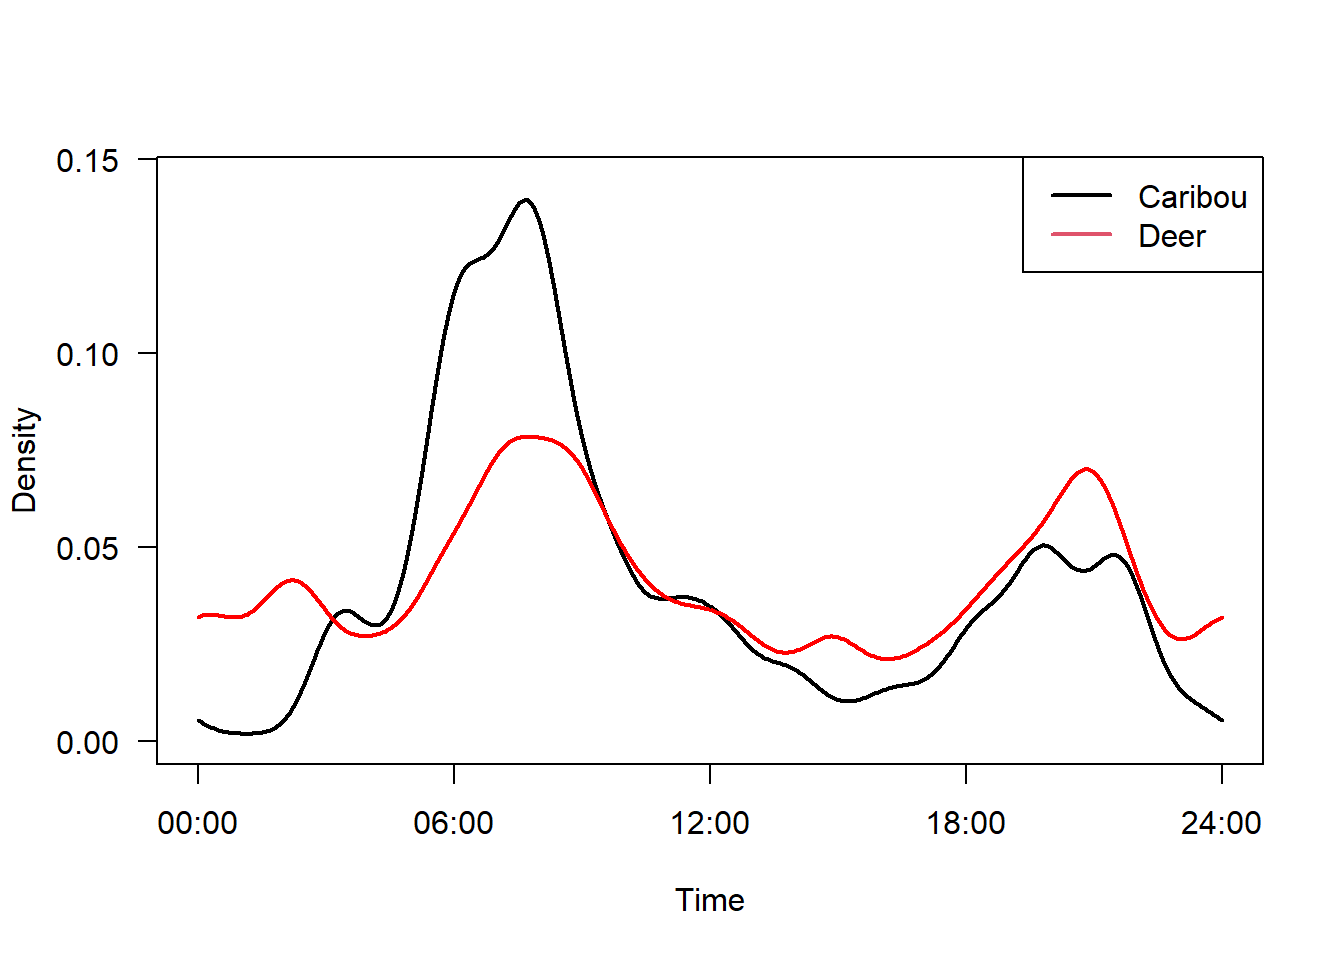
\includegraphics{bookdown-demo_files/figure-latex/unnamed-chunk-50-1.pdf}
Where each think black line is an active camera, and each thin grey box
represents each slice of the detection history.

We can create the detection histories using the following code:

\begin{Shaded}
\begin{Highlighting}[]
\KeywordTok{library}\NormalTok{(dplyr)}
\KeywordTok{library}\NormalTok{(tidyr)}
\KeywordTok{library}\NormalTok{(magrittr)}
\KeywordTok{library}\NormalTok{(tibble)}

\NormalTok{##Subset to your focal data}
\NormalTok{tmp <-}\StringTok{ }\NormalTok{weekObs[,}\KeywordTok{c}\NormalTok{(}\StringTok{"Deployment.Location.ID"}\NormalTok{, }\StringTok{"Date"}\NormalTok{, }\StringTok{"Odocoileus.virginianus"}\NormalTok{)]}

\CommentTok{# Turn the counts into presence/absence}
\NormalTok{tmp}\OperatorTok{$}\NormalTok{Odocoileus.virginianus[tmp}\OperatorTok{$}\NormalTok{Odocoileus.virginianus}\OperatorTok{>}\DecValTok{0}\NormalTok{] <-}\StringTok{ }\DecValTok{1}

\CommentTok{# Create a history}
\NormalTok{detHist <-}\StringTok{  }\NormalTok{tmp }\OperatorTok
\StringTok{  }\CommentTok{#Convert from long into wide format (a detection history) using spread}
\StringTok{  }\KeywordTok{spread}\NormalTok{(Date,Odocoileus.virginianus, }\DataTypeTok{fill =} \OtherTok{NA}\NormalTok{) }\OperatorTok\StringTok{ }
\StringTok{  }\CommentTok{# group by deployment location}
\StringTok{  }\KeywordTok{group_by}\NormalTok{(Deployment.Location.ID,) }\OperatorTok
\StringTok{  }\KeywordTok{column_to_rownames}\NormalTok{( }\DataTypeTok{var =} \StringTok{"Deployment.Location.ID"}\NormalTok{)}

\NormalTok{detHist <-}\StringTok{ }\KeywordTok{as.matrix}\NormalTok{(detHist)}
\end{Highlighting}
\end{Shaded}

The resulting data frame looks like this:

\begin{table}
\centering
\begin{tabular}[t]{l|r|r|r|r|r|r|r|r|r|r|r|r|r|r|r|r|r|r|r|r|r|r|r|r|r|r|r|r|r|r|r|r|r|r|r|r|r|r|r|r|r|r|r|r|r|r|r|r|r|r|r|r|r|r|r}
\hline
  & 2018-W45 & 2018-W46 & 2018-W47 & 2018-W48 & 2018-W49 & 2018-W50 & 2018-W51 & 2018-W52 & 2019-W00 & 2019-W01 & 2019-W02 & 2019-W03 & 2019-W04 & 2019-W05 & 2019-W06 & 2019-W07 & 2019-W08 & 2019-W09 & 2019-W10 & 2019-W11 & 2019-W12 & 2019-W13 & 2019-W14 & 2019-W15 & 2019-W16 & 2019-W17 & 2019-W18 & 2019-W19 & 2019-W20 & 2019-W21 & 2019-W22 & 2019-W23 & 2019-W24 & 2019-W25 & 2019-W26 & 2019-W27 & 2019-W28 & 2019-W29 & 2019-W30 & 2019-W31 & 2019-W32 & 2019-W33 & 2019-W34 & 2019-W35 & 2019-W36 & 2019-W37 & 2019-W38 & 2019-W39 & 2019-W40 & 2019-W41 & 2019-W42 & 2019-W43 & 2019-W44 & 2019-W45 & 2019-W46\\
\hline
Algar08 & 0 & 0 & 0 & 0 & 0 & 1 & 0 & 0 & 0 & 0 & 0 & 0 & 0 & 0 & 0 & 0 & 0 & 0 & 0 & 0 & 0 & 0 & 0 & 0 & 0 & 0 & 1 & 0 & 0 & 0 & 0 & 0 & 0 & 0 & 0 & 0 & 0 & 0 & 0 & 0 & 0 & 0 & 0 & 0 & 0 & 0 & 0 & 0 & 0 & 0 & 0 & 0 & 0 & 0 & 0\\
\hline
Algar27 & 1 & 0 & 0 & 0 & 0 & 0 & 0 & 0 & 0 & 0 & 0 & 0 & 0 & 0 & 0 & 0 & 0 & 0 & 0 & 0 & 0 & 0 & NA & NA & NA & NA & NA & NA & NA & NA & NA & NA & NA & NA & NA & NA & NA & NA & NA & NA & NA & NA & NA & NA & NA & NA & NA & NA & NA & NA & NA & NA & NA & NA & NA\\
\hline
Algar29 & 0 & 1 & 1 & 1 & 0 & 1 & 0 & 0 & 0 & 0 & 0 & 0 & 0 & 0 & 0 & 0 & 0 & 0 & 0 & 0 & 0 & 0 & 1 & 0 & 1 & 0 & 1 & 1 & 1 & 0 & 0 & 0 & 0 & 1 & 0 & 0 & 0 & 0 & 0 & 0 & 0 & 1 & 0 & 0 & 1 & 0 & 0 & 0 & 0 & 0 & 1 & 1 & 1 & 1 & 0\\
\hline
Algar31 & 0 & 0 & 0 & 0 & 0 & 0 & 0 & 0 & 0 & 0 & 0 & 0 & 0 & 0 & 0 & 0 & 0 & 0 & 0 & 0 & 0 & 0 & 0 & 0 & 0 & 0 & 0 & 0 & 0 & 0 & 0 & 1 & 0 & 0 & 0 & 0 & 0 & 0 & 0 & 0 & 0 & 0 & 0 & 0 & 0 & 0 & 0 & 0 & 0 & 0 & 0 & 0 & 0 & 0 & 0\\
\hline
Algar32 & 0 & 0 & 0 & 0 & 0 & 0 & 0 & 0 & 0 & 0 & 0 & 0 & 0 & 0 & 0 & 0 & 0 & 0 & 0 & 0 & 0 & 0 & 0 & 0 & 0 & 0 & 0 & 0 & 0 & 0 & 0 & 0 & 1 & 0 & 0 & 0 & 0 & 0 & 0 & 0 & 0 & 0 & 0 & 0 & 0 & 0 & 0 & 0 & 0 & 0 & 0 & 0 & 0 & 0 & 0\\
\hline
Algar34 & 0 & 0 & 1 & 0 & 0 & 0 & 0 & 0 & 0 & 0 & 1 & 0 & 0 & 0 & 0 & 0 & 0 & 0 & 0 & 0 & 0 & 0 & 0 & 0 & 0 & 0 & 0 & 0 & 0 & 0 & 0 & 0 & 0 & 0 & 0 & 0 & 0 & 0 & 0 & 0 & 0 & 0 & 0 & 0 & 0 & 0 & 0 & 0 & 0 & 0 & 0 & 0 & 0 & 0 & 0\\
\hline
Algar35 & 0 & 0 & 0 & 0 & 0 & 0 & 0 & 0 & 0 & 0 & 0 & 0 & 0 & 0 & 0 & 0 & 0 & 0 & 0 & 0 & 0 & 0 & 0 & 0 & 0 & 0 & 0 & 0 & 0 & 0 & 1 & 0 & 0 & 0 & 0 & 0 & 0 & 0 & 0 & 0 & 0 & 0 & 0 & 0 & 0 & 0 & 0 & 0 & 0 & 0 & 0 & 0 & 0 & 0 & 0\\
\hline
Algar37 & 0 & 0 & 0 & 0 & 0 & 0 & 0 & 0 & 0 & 0 & 0 & 0 & 0 & 0 & 0 & 0 & 0 & 0 & 0 & 0 & 0 & 0 & 0 & 0 & 0 & 0 & 0 & 0 & 0 & 0 & 0 & 0 & 0 & 0 & 0 & 0 & 0 & 0 & 0 & 0 & 0 & 0 & 0 & 0 & 0 & 0 & 0 & 0 & 0 & 0 & 0 & 0 & 0 & 0 & 0\\
\hline
Algar38 & 0 & 0 & 0 & 0 & 0 & 0 & 0 & 0 & 0 & 0 & 0 & 0 & 0 & 0 & 0 & 0 & 0 & 0 & 0 & 0 & 0 & 0 & 0 & 0 & 0 & 0 & 0 & 0 & 0 & 0 & 0 & 0 & 0 & 0 & 0 & 0 & 0 & 0 & 0 & 0 & 0 & 0 & 0 & 0 & 0 & 0 & 0 & 0 & 0 & 0 & 0 & 0 & 0 & 0 & 0\\
\hline
Algar39 & 0 & 0 & 0 & 0 & 0 & 0 & 0 & 0 & 0 & 0 & 0 & 0 & 0 & 0 & 0 & 0 & 0 & 0 & 0 & 0 & 0 & 0 & 0 & 0 & 0 & 0 & 0 & 0 & 0 & 0 & 0 & 0 & 0 & 0 & 0 & 0 & 0 & 0 & 0 & 0 & 0 & 0 & 0 & 0 & 0 & 0 & 0 & 0 & 0 & 0 & 0 & 0 & 0 & 0 & 0\\
\hline
Algar61 & 0 & 1 & 1 & 0 & 0 & 1 & 0 & 0 & 0 & 1 & 0 & 0 & 1 & 1 & 1 & 1 & 1 & 1 & 0 & 1 & 0 & 0 & 0 & 0 & 0 & 0 & 0 & 0 & 0 & 0 & 1 & 1 & 1 & 1 & 1 & 0 & 1 & 1 & 0 & 1 & 0 & 1 & 0 & 1 & 0 & 0 & 0 & 0 & 0 & 0 & 0 & 0 & 0 & 1 & 1\\
\hline
Algar62 & 0 & 0 & 0 & 0 & 0 & 0 & 1 & 1 & 0 & 1 & 0 & 1 & 1 & 0 & 0 & 0 & 0 & 0 & 0 & 0 & 0 & 0 & 1 & 1 & 1 & 1 & 0 & 0 & 1 & 1 & 1 & 1 & 1 & 1 & 0 & 1 & 0 & 0 & 0 & 0 & 0 & 1 & 1 & 1 & 1 & 0 & 0 & 0 & 0 & 0 & 0 & 0 & 0 & 0 & 0\\
\hline
Algar63 & 0 & 1 & 1 & 0 & 1 & 0 & 1 & 0 & 0 & 0 & 1 & 0 & 0 & 0 & 1 & 0 & 0 & 0 & 0 & 0 & 0 & 0 & 0 & 0 & 1 & 0 & 1 & 0 & 0 & 0 & 1 & 1 & 1 & 0 & 0 & 1 & 1 & 0 & 1 & 0 & 0 & 1 & 0 & 0 & 0 & 0 & 0 & 0 & 0 & 0 & 0 & 0 & 0 & 0 & 1\\
\hline
Algar64 & 0 & 0 & 0 & 0 & 0 & 0 & 0 & 0 & 0 & 0 & 0 & 0 & 0 & 0 & 0 & 0 & 0 & 0 & 0 & 0 & 0 & 0 & 0 & 0 & 0 & 0 & 0 & 0 & 0 & 0 & 0 & 0 & 0 & 0 & 0 & 0 & 0 & 0 & 0 & 0 & 0 & 0 & 0 & 0 & 0 & 0 & 0 & 0 & 0 & 0 & 0 & 0 & 0 & 0 & 0\\
\hline
Algar65 & 0 & 0 & 0 & 0 & 0 & 0 & 0 & 0 & 0 & 0 & 0 & 0 & 0 & 0 & 0 & 0 & 0 & 0 & 0 & 0 & 0 & 0 & 0 & 0 & 0 & 0 & 0 & 0 & 0 & 0 & 0 & 0 & 0 & 0 & NA & NA & NA & NA & NA & NA & NA & NA & NA & NA & NA & NA & NA & NA & NA & NA & NA & NA & NA & NA & NA\\
\hline
Algar66 & 0 & 0 & 0 & 0 & 0 & 0 & 0 & 0 & 0 & 0 & 0 & 0 & 0 & 0 & 0 & 0 & 0 & 0 & 0 & 0 & 0 & 0 & 0 & 0 & 0 & 0 & 0 & 0 & 0 & 0 & 0 & 0 & 0 & 0 & 1 & 0 & 0 & 0 & 0 & 0 & 0 & 0 & 0 & 0 & 0 & 0 & 0 & 0 & 0 & 0 & 0 & 0 & 0 & 0 & 0\\
\hline
Algar67 & 0 & 0 & 0 & 0 & 0 & 0 & 0 & 0 & 0 & 0 & 0 & 0 & 0 & 0 & 0 & 0 & 0 & 0 & 0 & 0 & 0 & 0 & 0 & 0 & 0 & 0 & 1 & 0 & 0 & 0 & 1 & 0 & 0 & 0 & 0 & 0 & 1 & 0 & 0 & 0 & 0 & 0 & 0 & 0 & 0 & 0 & 0 & 0 & 0 & 0 & 0 & 0 & 0 & 0 & 0\\
\hline
Algar68 & 0 & 0 & 0 & 0 & 0 & 0 & 0 & 0 & 0 & 0 & 0 & 0 & 0 & 0 & 0 & 0 & 0 & 0 & 0 & 0 & 0 & 0 & 0 & 0 & 0 & 0 & 0 & 0 & 0 & 0 & 0 & 0 & 0 & 0 & 0 & 0 & 0 & 0 & 0 & 0 & 0 & 0 & 0 & 0 & 0 & 0 & 0 & 0 & 0 & 0 & 0 & 0 & 0 & 0 & 0\\
\hline
Algar69 & 1 & 1 & 0 & 1 & 1 & 1 & 0 & 0 & 0 & 0 & 0 & 0 & 0 & 0 & 0 & 0 & 0 & 0 & 0 & 0 & 0 & 1 & 0 & 1 & 1 & 0 & 1 & 0 & 0 & 0 & 0 & 0 & 0 & 1 & 0 & 0 & 1 & 1 & 1 & 0 & 1 & 1 & 1 & 1 & 0 & 0 & 1 & 1 & 1 & 1 & 1 & 0 & 0 & 1 & 1\\
\hline
Algar70 & 0 & 0 & 0 & 0 & 0 & 0 & 0 & 0 & 0 & 0 & 0 & 0 & 0 & 0 & 0 & 0 & 0 & 0 & 0 & 0 & 0 & 0 & 0 & 0 & 0 & 0 & 0 & 0 & 0 & 0 & 0 & 0 & 1 & 0 & 1 & 0 & 0 & 0 & 1 & 0 & 1 & 0 & 0 & 0 & 0 & 0 & 0 & 0 & 0 & 0 & 0 & 0 & 0 & 0 & 0\\
\hline
\end{tabular}
\end{table}

It is a matrix of all the dates the cameras were active, and whether the
species was present or absent on that day. It should mirror the camera
activity plot above. The \texttt{fill\ =\ NA} command puts a zero where
there is data for a given day. However, we have lost our effort
information - the number of days each camera was active in a given time
period.

To keep that information we also create an effort history
\texttt{effHist}:

\begin{Shaded}
\begin{Highlighting}[]
\CommentTok{# To create the effort matrix - inst of the Focal Species bring in the effort}
\NormalTok{effDat <-}\StringTok{ }\NormalTok{weekObs[,}\KeywordTok{c}\NormalTok{(}\StringTok{"Deployment.Location.ID"}\NormalTok{, }\StringTok{"Date"}\NormalTok{, }\StringTok{"Effort"}\NormalTok{)]}

\NormalTok{effHist <-}\StringTok{  }\NormalTok{effDat }\OperatorTok
\StringTok{  }\CommentTok{# Create a matrix based on dates and effort}
\StringTok{  }\KeywordTok{spread}\NormalTok{(Date,Effort, }\DataTypeTok{fill =} \OtherTok{NA}\NormalTok{) }\OperatorTok\StringTok{ }
\StringTok{  }\CommentTok{# group by deloyment Location ID, then make that the row.namesd}
\StringTok{  }\KeywordTok{group_by}\NormalTok{(Deployment.Location.ID,) }\OperatorTok
\StringTok{  }\KeywordTok{column_to_rownames}\NormalTok{( }\DataTypeTok{var =} \StringTok{"Deployment.Location.ID"}\NormalTok{) }

\NormalTok{effHist <-}\StringTok{ }\KeywordTok{as.matrix}\NormalTok{(effHist)}
\end{Highlighting}
\end{Shaded}

Check that it looks sensible:

\begin{table}
\centering
\begin{tabular}[t]{l|r|r|r|r|r|r|r|r|r|r|r|r|r|r|r|r|r|r|r|r|r|r|r|r|r|r|r|r|r|r|r|r|r|r|r|r|r|r|r|r|r|r|r|r|r|r|r|r|r|r|r|r|r|r|r}
\hline
  & 2018-W45 & 2018-W46 & 2018-W47 & 2018-W48 & 2018-W49 & 2018-W50 & 2018-W51 & 2018-W52 & 2019-W00 & 2019-W01 & 2019-W02 & 2019-W03 & 2019-W04 & 2019-W05 & 2019-W06 & 2019-W07 & 2019-W08 & 2019-W09 & 2019-W10 & 2019-W11 & 2019-W12 & 2019-W13 & 2019-W14 & 2019-W15 & 2019-W16 & 2019-W17 & 2019-W18 & 2019-W19 & 2019-W20 & 2019-W21 & 2019-W22 & 2019-W23 & 2019-W24 & 2019-W25 & 2019-W26 & 2019-W27 & 2019-W28 & 2019-W29 & 2019-W30 & 2019-W31 & 2019-W32 & 2019-W33 & 2019-W34 & 2019-W35 & 2019-W36 & 2019-W37 & 2019-W38 & 2019-W39 & 2019-W40 & 2019-W41 & 2019-W42 & 2019-W43 & 2019-W44 & 2019-W45 & 2019-W46\\
\hline
Algar08 & 1 & 7 & 7 & 7 & 7 & 7 & 7 & 2 & 5 & 7 & 7 & 7 & 7 & 7 & 7 & 7 & 7 & 7 & 7 & 7 & 7 & 7 & 7 & 7 & 7 & 7 & 7 & 7 & 7 & 7 & 7 & 7 & 7 & 7 & 7 & 7 & 7 & 7 & 7 & 7 & 7 & 7 & 7 & 7 & 7 & 7 & 7 & 7 & 7 & 7 & 7 & 7 & 7 & 7 & 5\\
\hline
Algar27 & 3 & 7 & 7 & 7 & 7 & 7 & 7 & 2 & 5 & 7 & 7 & 7 & 7 & 7 & 7 & 7 & 7 & 7 & 7 & 7 & 7 & 4 & NA & NA & NA & NA & NA & NA & NA & NA & NA & NA & NA & NA & NA & NA & NA & NA & NA & NA & NA & NA & NA & NA & NA & NA & NA & NA & NA & NA & NA & NA & NA & NA & NA\\
\hline
Algar29 & 3 & 7 & 7 & 7 & 7 & 7 & 7 & 2 & 5 & 7 & 7 & 7 & 7 & 7 & 7 & 7 & 7 & 7 & 7 & 7 & 7 & 7 & 7 & 7 & 7 & 7 & 7 & 7 & 7 & 7 & 7 & 7 & 7 & 7 & 7 & 7 & 7 & 7 & 7 & 7 & 7 & 7 & 7 & 7 & 7 & 7 & 7 & 7 & 7 & 7 & 7 & 7 & 7 & 7 & 4\\
\hline
Algar31 & 2 & 7 & 7 & 7 & 7 & 7 & 7 & 2 & 5 & 7 & 7 & 7 & 7 & 7 & 7 & 7 & 7 & 7 & 7 & 7 & 7 & 7 & 7 & 7 & 7 & 7 & 7 & 7 & 7 & 7 & 7 & 7 & 7 & 7 & 7 & 7 & 7 & 7 & 7 & 7 & 7 & 7 & 7 & 7 & 7 & 7 & 7 & 7 & 7 & 7 & 7 & 7 & 7 & 7 & 5\\
\hline
Algar32 & 4 & 7 & 7 & 7 & 7 & 7 & 7 & 2 & 5 & 7 & 7 & 7 & 7 & 7 & 7 & 7 & 7 & 7 & 7 & 7 & 7 & 7 & 7 & 7 & 7 & 7 & 7 & 7 & 7 & 7 & 7 & 7 & 7 & 7 & 7 & 7 & 7 & 7 & 7 & 7 & 7 & 7 & 7 & 7 & 7 & 7 & 7 & 7 & 7 & 7 & 7 & 7 & 7 & 7 & 3\\
\hline
Algar34 & 1 & 7 & 7 & 7 & 7 & 7 & 7 & 2 & 5 & 7 & 7 & 7 & 7 & 7 & 7 & 7 & 7 & 7 & 7 & 7 & 7 & 7 & 7 & 7 & 7 & 7 & 7 & 7 & 7 & 7 & 7 & 7 & 7 & 7 & 7 & 7 & 7 & 7 & 7 & 7 & 7 & 7 & 7 & 7 & 7 & 7 & 7 & 7 & 7 & 7 & 7 & 7 & 7 & 7 & 5\\
\hline
Algar35 & 3 & 7 & 7 & 7 & 7 & 7 & 7 & 2 & 5 & 7 & 7 & 7 & 7 & 7 & 7 & 7 & 7 & 7 & 7 & 7 & 7 & 7 & 7 & 7 & 7 & 7 & 7 & 7 & 7 & 7 & 7 & 7 & 7 & 7 & 7 & 7 & 7 & 7 & 7 & 7 & 7 & 7 & 7 & 7 & 7 & 7 & 7 & 7 & 7 & 7 & 7 & 7 & 7 & 7 & 6\\
\hline
Algar37 & 1 & 7 & 7 & 7 & 7 & 7 & 7 & 2 & 5 & 7 & 7 & 7 & 7 & 7 & 7 & 7 & 7 & 7 & 7 & 7 & 7 & 7 & 7 & 7 & 7 & 7 & 7 & 7 & 7 & 7 & 7 & 7 & 7 & 7 & 7 & 7 & 7 & 7 & 7 & 7 & 7 & 7 & 7 & 7 & 7 & 7 & 7 & 7 & 7 & 7 & 7 & 7 & 7 & 7 & 5\\
\hline
Algar38 & 2 & 7 & 7 & 7 & 7 & 7 & 7 & 2 & 5 & 7 & 7 & 7 & 7 & 7 & 7 & 7 & 7 & 7 & 7 & 7 & 7 & 7 & 7 & 7 & 7 & 7 & 7 & 7 & 7 & 7 & 7 & 7 & 7 & 7 & 7 & 7 & 7 & 7 & 7 & 7 & 7 & 7 & 7 & 7 & 7 & 7 & 7 & 7 & 7 & 7 & 7 & 7 & 7 & 7 & 5\\
\hline
Algar39 & 2 & 7 & 7 & 7 & 7 & 7 & 7 & 2 & 5 & 7 & 7 & 7 & 7 & 7 & 7 & 7 & 7 & 7 & 7 & 7 & 7 & 7 & 7 & 7 & 7 & 7 & 7 & 7 & 7 & 7 & 7 & 7 & 7 & 7 & 7 & 7 & 7 & 7 & 7 & 7 & 7 & 7 & 7 & 7 & 7 & 7 & 7 & 7 & 7 & 7 & 7 & 7 & 7 & 7 & 3\\
\hline
Algar61 & 1 & 7 & 7 & 7 & 7 & 7 & 7 & 2 & 5 & 7 & 7 & 7 & 7 & 7 & 7 & 7 & 7 & 7 & 7 & 7 & 7 & 7 & 7 & 7 & 7 & 7 & 7 & 7 & 7 & 7 & 7 & 7 & 7 & 7 & 7 & 7 & 7 & 7 & 7 & 7 & 7 & 7 & 7 & 7 & 7 & 7 & 7 & 7 & 7 & 7 & 7 & 7 & 7 & 7 & 3\\
\hline
Algar62 & 1 & 7 & 7 & 7 & 7 & 7 & 7 & 2 & 5 & 7 & 7 & 7 & 7 & 7 & 7 & 7 & 7 & 7 & 7 & 7 & 7 & 7 & 7 & 7 & 7 & 7 & 7 & 7 & 7 & 7 & 7 & 7 & 7 & 7 & 7 & 7 & 7 & 7 & 7 & 7 & 7 & 7 & 7 & 7 & 7 & 7 & 7 & 7 & 7 & 7 & 7 & 7 & 7 & 7 & 5\\
\hline
Algar63 & 2 & 7 & 7 & 7 & 7 & 7 & 7 & 2 & 5 & 7 & 7 & 7 & 7 & 7 & 7 & 7 & 7 & 7 & 7 & 7 & 7 & 7 & 7 & 7 & 7 & 7 & 7 & 7 & 7 & 7 & 7 & 7 & 7 & 7 & 7 & 7 & 7 & 7 & 7 & 7 & 7 & 7 & 7 & 7 & 7 & 7 & 7 & 7 & 7 & 7 & 7 & 7 & 7 & 7 & 5\\
\hline
Algar64 & 1 & 7 & 7 & 7 & 7 & 7 & 7 & 2 & 5 & 7 & 7 & 7 & 7 & 7 & 7 & 7 & 7 & 7 & 7 & 7 & 7 & 7 & 7 & 7 & 7 & 7 & 7 & 7 & 7 & 7 & 7 & 7 & 7 & 7 & 7 & 7 & 7 & 7 & 7 & 7 & 7 & 7 & 7 & 7 & 7 & 7 & 7 & 7 & 7 & 7 & 7 & 7 & 7 & 7 & 5\\
\hline
Algar65 & 2 & 7 & 7 & 7 & 7 & 7 & 7 & 2 & 5 & 7 & 7 & 7 & 7 & 7 & 7 & 7 & 7 & 7 & 7 & 7 & 7 & 7 & 7 & 7 & 7 & 7 & 7 & 7 & 7 & 7 & 7 & 7 & 7 & 6 & NA & NA & NA & NA & NA & NA & NA & NA & NA & NA & NA & NA & NA & NA & NA & NA & NA & NA & NA & NA & NA\\
\hline
Algar66 & 2 & 7 & 7 & 7 & 7 & 7 & 7 & 2 & 5 & 7 & 7 & 7 & 7 & 7 & 7 & 7 & 7 & 7 & 7 & 7 & 7 & 7 & 7 & 7 & 7 & 7 & 7 & 7 & 7 & 7 & 7 & 7 & 7 & 7 & 7 & 7 & 7 & 7 & 7 & 7 & 7 & 7 & 7 & 7 & 7 & 7 & 7 & 7 & 7 & 7 & 7 & 7 & 7 & 7 & 3\\
\hline
Algar67 & 3 & 7 & 7 & 7 & 7 & 7 & 7 & 2 & 5 & 7 & 7 & 7 & 7 & 7 & 7 & 7 & 7 & 7 & 7 & 7 & 7 & 7 & 7 & 7 & 7 & 7 & 7 & 7 & 7 & 7 & 7 & 7 & 7 & 7 & 7 & 7 & 7 & 7 & 7 & 7 & 7 & 7 & 7 & 7 & 7 & 7 & 7 & 7 & 7 & 7 & 7 & 7 & 7 & 7 & 4\\
\hline
Algar68 & 3 & 7 & 7 & 7 & 7 & 7 & 7 & 2 & 5 & 7 & 7 & 7 & 7 & 7 & 7 & 7 & 7 & 7 & 7 & 7 & 7 & 7 & 7 & 7 & 7 & 7 & 7 & 7 & 7 & 7 & 7 & 7 & 7 & 7 & 7 & 7 & 7 & 7 & 7 & 7 & 7 & 7 & 7 & 7 & 7 & 7 & 7 & 7 & 7 & 7 & 7 & 7 & 7 & 7 & 4\\
\hline
Algar69 & 4 & 7 & 7 & 7 & 7 & 7 & 7 & 2 & 5 & 7 & 7 & 7 & 7 & 7 & 7 & 7 & 7 & 7 & 7 & 7 & 7 & 7 & 7 & 7 & 7 & 7 & 7 & 7 & 7 & 7 & 7 & 7 & 7 & 7 & 7 & 7 & 7 & 7 & 7 & 7 & 7 & 7 & 7 & 7 & 7 & 7 & 7 & 7 & 7 & 7 & 7 & 7 & 7 & 7 & 3\\
\hline
Algar70 & 4 & 7 & 7 & 7 & 7 & 7 & 7 & 2 & 5 & 7 & 7 & 7 & 7 & 7 & 7 & 7 & 7 & 7 & 7 & 7 & 7 & 7 & 7 & 7 & 7 & 7 & 7 & 7 & 7 & 7 & 7 & 7 & 7 & 7 & 7 & 7 & 7 & 7 & 7 & 7 & 7 & 7 & 7 & 7 & 7 & 7 & 7 & 7 & 7 & 7 & 7 & 7 & 7 & 7 & 3\\
\hline
\end{tabular}
\end{table}

Remove weeks w/0 full sample?

\begin{Shaded}
\begin{Highlighting}[]
\NormalTok{detHist[effHist}\OperatorTok{!=}\DecValTok{7}\NormalTok{] <-}\StringTok{ }\OtherTok{NA}
\end{Highlighting}
\end{Shaded}

\subsection{unmarked package}\label{unmarked-package}

\begin{Shaded}
\begin{Highlighting}[]
\KeywordTok{library}\NormalTok{(unmarked)}
\NormalTok{sta <-}\StringTok{ }\KeywordTok{read.csv}\NormalTok{(}\StringTok{"data/raw_data/Example_station_data.csv"}\NormalTok{, }\DataTypeTok{header=}\NormalTok{T)}
\CommentTok{# Unmarked wants your detection history, effort data and site covariates as matrices.}

\CommentTok{# Build an unmarkedFramOccu}
\NormalTok{unDat <-}\StringTok{ }\KeywordTok{unmarkedFrameOccu}\NormalTok{(}\DataTypeTok{y =}\NormalTok{ detHist,}
                          \CommentTok{# siteCovs = dataframe with site rows x column variables (in same order as detHist)}
                           \DataTypeTok{siteCovs =}\NormalTok{ sta) }
\end{Highlighting}
\end{Shaded}

\begin{verbatim}
## Warning: siteCovs contains characters. Converting them to factors.
\end{verbatim}

\begin{Shaded}
\begin{Highlighting}[]
\CommentTok{# Fit general model all variables}
\NormalTok{m1 <-}\StringTok{ }\KeywordTok{occu}\NormalTok{(}\DataTypeTok{formula =} \OperatorTok{~}\DecValTok{1} \CommentTok{# detection formula first}
                     \OperatorTok{~}\NormalTok{LOW500, }\CommentTok{# occupancy formula second,}
                \DataTypeTok{data =}\NormalTok{ unDat)}
\end{Highlighting}
\end{Shaded}

\begin{Shaded}
\begin{Highlighting}[]
\KeywordTok{summary}\NormalTok{(m1)}
\end{Highlighting}
\end{Shaded}

\begin{verbatim}
## 
## Call:
## occu(formula = ~1 ~ LOW500, data = unDat)
## 
## Occupancy (logit-scale):
##             Estimate  SE     z P(>|z|)
## (Intercept)     6.15 2.9  2.12  0.0339
## LOW500         -7.39 3.6 -2.05  0.0405
## 
## Detection (logit-scale):
##  Estimate    SE     z P(>|z|)
##     -1.63 0.106 -15.4 9.8e-54
## 
## AIC: 617.8133 
## Number of sites: 20
## optim convergence code: 0
## optim iterations: 45 
## Bootstrap iterations: 0
\end{verbatim}

\begin{Shaded}
\begin{Highlighting}[]
\CommentTok{# Generate new data to predict from }
\NormalTok{newDat <-}\StringTok{ }\KeywordTok{cbind}\NormalTok{(}\KeywordTok{expand.grid}\NormalTok{(}\DataTypeTok{LOW500=}\KeywordTok{seq}\NormalTok{(}\KeywordTok{min}\NormalTok{(sta}\OperatorTok{$}\NormalTok{LOW500),}\KeywordTok{max}\NormalTok{(sta}\OperatorTok{$}\NormalTok{LOW500), }\DataTypeTok{length.out=}\DecValTok{100}\NormalTok{)))}

\NormalTok{newDat <-}\StringTok{ }\KeywordTok{predict}\NormalTok{(m1, }\DataTypeTok{type=}\StringTok{"state"}\NormalTok{, }\DataTypeTok{newdata =}\NormalTok{ newDat, }\DataTypeTok{appendData=}\OtherTok{TRUE}\NormalTok{)}

\NormalTok{p1 <-}\StringTok{ }\KeywordTok{ggplot}\NormalTok{(newDat, }\KeywordTok{aes}\NormalTok{(}\DataTypeTok{x =}\NormalTok{ LOW500, }\DataTypeTok{y =}\NormalTok{ Predicted)) }\OperatorTok{+}
\StringTok{  }\KeywordTok{geom_ribbon}\NormalTok{(}\KeywordTok{aes}\NormalTok{(}\DataTypeTok{ymin =}\NormalTok{ lower, }\DataTypeTok{ymax =}\NormalTok{ upper), }\DataTypeTok{alpha =} \FloatTok{0.5}\NormalTok{, }\DataTypeTok{linetype =} \StringTok{"dashed"}\NormalTok{) }\OperatorTok{+}
\StringTok{  }\KeywordTok{geom_path}\NormalTok{(}\DataTypeTok{size =} \DecValTok{1}\NormalTok{) }\OperatorTok{+}
\StringTok{  }\KeywordTok{labs}\NormalTok{(}\DataTypeTok{x =} \StringTok{"Proportion lowland habitat"}\NormalTok{, }\DataTypeTok{y =} \StringTok{"Occupancy probability"}\NormalTok{) }\OperatorTok{+}
\StringTok{  }\KeywordTok{theme_classic}\NormalTok{() }\OperatorTok{+}
\StringTok{  }\KeywordTok{coord_cartesian}\NormalTok{(}\DataTypeTok{ylim =} \KeywordTok{c}\NormalTok{(}\DecValTok{0}\NormalTok{,}\DecValTok{1}\NormalTok{))}

\NormalTok{p1}
\end{Highlighting}
\end{Shaded}

\includegraphics{bookdown-demo_files/figure-latex/unnamed-chunk-59-1.pdf}

\section{Multispecies occupancy
model}\label{multispecies-occupancy-model-1}

Coming soon!

\chapter{Density}\label{density}

There is an explosion in the number of frameowrk looking to hit what is
considered the gold stardard in many ecological surveys - population
density information.

\textbf{Key resources}

{[}Gilbert, Neil A., et al. ``Abundance estimation of unmarked animals
based on camera‐trap data.'' Conservation Biology 35.1 (2021):
88-100{]}(173-181.{]}(\url{https://conbio.onlinelibrary.wiley.com/doi/epdf/10.1111/cobi.13517})

\chapter{Activity}\label{activity}

Given that camera traps record the time of the photo, they represent a
powerful tool to explore and contrast the acivity pattterns of the
species they detect. Such analyses can give insight into ompetition,
predation and coexistance.

\emph{Must read}
\href{https://zslpublications.onlinelibrary.wiley.com/doi/full/10.1002/rse2.60}{Frey,
Sandra, et al. ``Investigating animal activity patterns and temporal
niche partitioning using camera‐trap data: Challenges and
opportunities.'' Remote Sensing in Ecology and Conservation 3.3 (2017):
123-132.}

Two key packages

\begin{itemize}
\tightlist
\item
  \texttt{overlap}
  \url{https://cran.r-project.org/web/packages/overlap/index.html}
\item
  \texttt{activity}
  \url{https://cran.r-project.org/web/packages/activity/index.html}
\end{itemize}

\section{Example}\label{example}

To demonstrate how we might investigate temporal niche partitioning, we
will be working from the independent observations data frame.

\begin{Shaded}
\begin{Highlighting}[]
\CommentTok{# Import the data}
\NormalTok{dat <-}\StringTok{ }\KeywordTok{read.csv}\NormalTok{(}\StringTok{"data/processed_data/Algar_30min_Independent.csv"}\NormalTok{, }\DataTypeTok{header=}\NormalTok{T)}
\end{Highlighting}
\end{Shaded}

Which looks like this:

\begin{table}
\centering
\begin{tabular}[t]{l|l|l|l|l|l|r|r|l|l|l|r|r|r}
\hline
Project.ID & Deployment.Location.ID & Species & Date\_Time.Captured & Age & Sex & Number.of.Animals & Minimum.Group.Size & Behaviour & Blank & Event.ID & Event.Duration & Event.Groupsize & Event.Observations\\
\hline
Algar & Algar08 & Odocoileus virginianus & 2018-12-18 20:54:56 & Adult & Male & 1 & 1 & Travelling & FALSE & E0 & 15 & 1 & 7\\
\hline
Algar & Algar08 & Alces alces & 2019-04-20 14:37:51 & Adult &  & 1 & 2 & Travelling & FALSE & E1 & 57 & 2 & 10\\
\hline
Algar & Algar08 & Alces alces & 2019-04-21 19:58:59 & Unidentified &  & 2 & 2 &  & FALSE & E2 & 58 & 2 & 11\\
\hline
Algar & Algar08 & Odocoileus virginianus & 2019-05-07 09:43:59 & Adult &  & 1 & 1 & Travelling & FALSE & E3 & 5 & 1 & 4\\
\hline
Algar & Algar08 & Rangifer tarandus & 2019-05-23 08:31:29 & Unidentified &  & 1 & 2 & Travelling & FALSE & E4 & 34 & 2 & 9\\
\hline
Algar & Algar08 & Alces alces & 2019-08-04 05:31:51 & Unidentified &  & 1 & 2 & Travelling & FALSE & E5 & 4 & 2 & 4\\
\hline
\end{tabular}
\end{table}

Then load the activity package.

\begin{Shaded}
\begin{Highlighting}[]
\CommentTok{# Import the data}
\KeywordTok{library}\NormalTok{(activity) }\CommentTok{# estimate radial time}
\end{Highlighting}
\end{Shaded}

We first need to convert the ``time'' in our datasets into radian time
(on the range {[}0, 2*pi{]}) and proportion time (on the range 0-1):

\begin{Shaded}
\begin{Highlighting}[]
\CommentTok{#Radian time}
\NormalTok{dat}\OperatorTok{$}\NormalTok{rtime <-}\StringTok{ }\KeywordTok{gettime}\NormalTok{(dat}\OperatorTok{$}\NormalTok{Date_Time.Captured, }\StringTok{"%Y-%m-%d %H:%M:%S"}\NormalTok{)}
\end{Highlighting}
\end{Shaded}

Then fit the basic activity models available in the package. Note, more
complex models are available, including accountting for the fact that
the detection distance of camera traps varies from night to day. Here we
will keep this simple!

\textbf{White-tailed deer}

\begin{Shaded}
\begin{Highlighting}[]
\NormalTok{m1 <-}\StringTok{ }\KeywordTok{fitact}\NormalTok{(dat}\OperatorTok{$}\NormalTok{rtime[dat}\OperatorTok{$}\NormalTok{Species}\OperatorTok{==}\StringTok{"Odocoileus virginianus"}\NormalTok{])}
\KeywordTok{plot}\NormalTok{(m1)}
\end{Highlighting}
\end{Shaded}

\includegraphics{bookdown-demo_files/figure-latex/unnamed-chunk-66-1.pdf}

\textbf{Caribou}

\begin{Shaded}
\begin{Highlighting}[]
\NormalTok{m2 <-}\StringTok{ }\KeywordTok{fitact}\NormalTok{(dat}\OperatorTok{$}\NormalTok{rtime[dat}\OperatorTok{$}\NormalTok{Species}\OperatorTok{==}\StringTok{"Rangifer tarandus"}\NormalTok{])}
\KeywordTok{plot}\NormalTok{(m2)}
\end{Highlighting}
\end{Shaded}

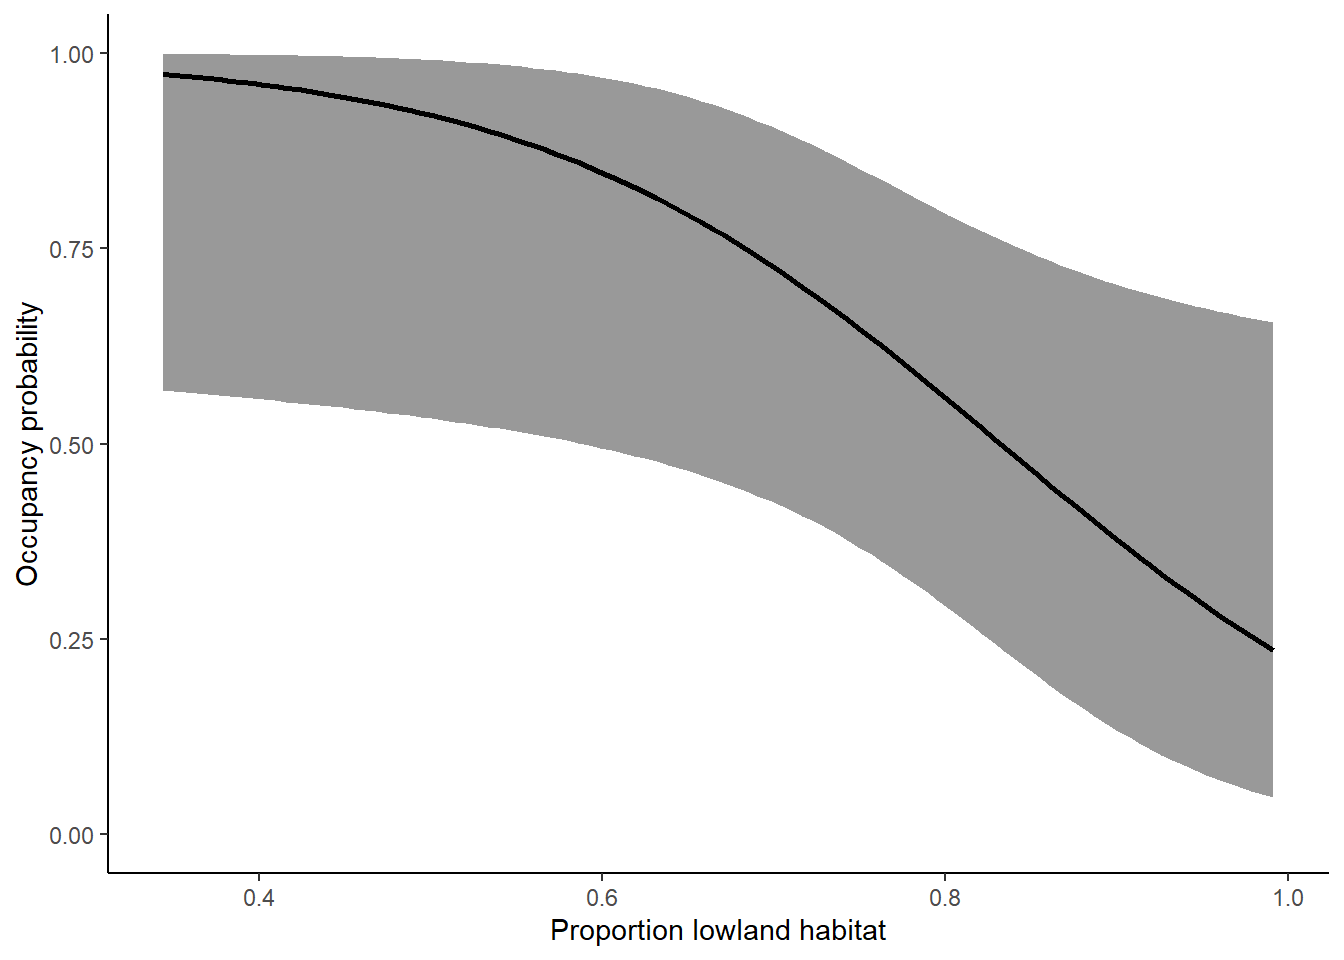
\includegraphics{bookdown-demo_files/figure-latex/unnamed-chunk-67-1.pdf}

We can compare the activity plots of both species on the same axis
visually:

\begin{Shaded}
\begin{Highlighting}[]
\CommentTok{# Plot both on the same axis}

\KeywordTok{plot}\NormalTok{(m1, }\DataTypeTok{yunit=}\StringTok{"density"}\NormalTok{, }\DataTypeTok{data=}\StringTok{"none"}\NormalTok{, }\DataTypeTok{ylim=}\KeywordTok{c}\NormalTok{(}\DecValTok{0}\NormalTok{,}\FloatTok{0.1}\NormalTok{), }\DataTypeTok{las=}\DecValTok{1}\NormalTok{, }\DataTypeTok{lwd=}\DecValTok{2}\NormalTok{)}
\KeywordTok{plot}\NormalTok{(m2, }\DataTypeTok{yunit=}\StringTok{"density"}\NormalTok{, }\DataTypeTok{data=}\StringTok{"none"}\NormalTok{, }\DataTypeTok{add=}\OtherTok{TRUE}\NormalTok{, }\DataTypeTok{tline=}\KeywordTok{list}\NormalTok{(}\DataTypeTok{col=}\StringTok{"red"}\NormalTok{))}
\KeywordTok{legend}\NormalTok{(}\StringTok{"topleft"}\NormalTok{, }\KeywordTok{c}\NormalTok{(}\StringTok{"White tailed deer"}\NormalTok{, }\StringTok{"Caribou"}\NormalTok{), }\DataTypeTok{col=}\DecValTok{1}\OperatorTok{:}\DecValTok{2}\NormalTok{, }\DataTypeTok{lty=}\DecValTok{1}\NormalTok{)}
\end{Highlighting}
\end{Shaded}

\includegraphics{bookdown-demo_files/figure-latex/unnamed-chunk-68-1.pdf}

We can compare different activity patterns using coefficient of overlap
(∆) - devleoped by Ridout and Linkie. The coefficient ranges from 0 (no
overlap) to 1 (complete overlap). We can implement for a two species
comparison as follows:

\begin{Shaded}
\begin{Highlighting}[]
\CommentTok{# Note reps reduced to speed up running time}
\KeywordTok{compareCkern}\NormalTok{(m1, m2, }\DataTypeTok{reps =} \DecValTok{250}\NormalTok{)}
\end{Highlighting}
\end{Shaded}

\begin{verbatim}
##        obs       null     seNull      pNull 
## 0.79074068 0.84462622 0.03705724 0.08400000
\end{verbatim}

The output above represents: obs = observed overlap index; null = mean
null overlap index; seNull = standard error of the null distribution;
pNull = probability observed index arose by chance.

Which suggets that there is no significant different between our two
species, perhaps not surprising given that they spatially degregate not
temporally.

\subsection{Other examples}\label{other-examples}

Houngbégnon, Fructueux GA, et al. ``Daily Activity Patterns and
Co-Occurrence of Duikers Revealed by an Intensive Camera Trap Survey
across Central African Rainforests.'' Animals 10.12 (2020): 2200.
\url{https://pubmed.ncbi.nlm.nih.gov/33255400/}

Ross J, Hearn AJ, Johnson PJ, Macdonald DW (2013). \Activity patterns
and temporal avoidance by prey in response to Sunda clouded leopard
predation risk." Journal of Zoology, 290(2), 96\{106.

Ramesh T, Kalle R, Sankar K, Qureshi Q (2012). \Spatio-temporal
partitioning among large carnivores in relation to major prey species in
Western Ghats." Journal of Zoology, 287(4), 269\{275.

Azevedo FC, Lemos FG, Freitas-Junior MC, Rocha DG, Azevedo FCC (2018).
\Puma activity patterns and temporal overlap with prey in a
human-modied landscape at Southeastern Brazil." Journal of Zoology,

\chapter{Phenology}\label{phenology}

Phenopix is an R package which allows the user to extract visual
information from time lapse images. It provides a quantitative daily
measure of vegetation phenology at each site (e.g.~green-up, senescence,
snow cover)

The Phenopix package has a five step process: i) a region of interest
(ROI) is identified; ii) the red, green, and blue digital numbers from
each image in the timeseries is extracted and an index of relative
`greenness' is computed and plotted from the digital numbers; iii) the
vegetation indices' data points are filtered to remove inconsistencies;
iv) a curve is fit to the data and phenophases are determined from the
curve; v) and phenophase uncertainties are calculated.

\section{Worked example}\label{worked-example}

Coming soon. Check the \href{https://github.com/WildCoLab}{wildCo github
page for updates}

\chapter{Phenology}\label{phenology-1}

Phenopix is an R package which allows the user to extract visual
information from time lapse images. It provides a quantitative daily
measure of vegetation phenology at each site (e.g.~green-up, senescence,
snow cover)

The Phenopix package has a five step process: i) a region of interest
(ROI) is identified; ii) the red, green, and blue digital numbers from
each image in the timeseries is extracted and an index of relative
`greenness' is computed and plotted from the digital numbers; iii) the
vegetation indices' data points are filtered to remove inconsistencies;
iv) a curve is fit to the data and phenophases are determined from the
curve; v) and phenophase uncertainties are calculated.

\section{Worked example}\label{worked-example-1}

Coming soon. Check the \href{https://github.com/WildCoLab}{wildCo github
page for updates}

\chapter{Phenology}\label{phenology-2}

Phenopix is an R package which allows the user to extract visual
information from time lapse images. It provides a quantitative daily
measure of vegetation phenology at each site (e.g.~green-up, senescence,
snow cover)

The Phenopix package has a five step process: i) a region of interest
(ROI) is identified; ii) the red, green, and blue digital numbers from
each image in the timeseries is extracted and an index of relative
`greenness' is computed and plotted from the digital numbers; iii) the
vegetation indices' data points are filtered to remove inconsistencies;
iv) a curve is fit to the data and phenophases are determined from the
curve; v) and phenophase uncertainties are calculated.

\section{Worked example}\label{worked-example-2}

Coming soon. Check the \href{https://github.com/WildCoLab}{wildCo github
page for updates}

\chapter{Phenology}\label{phenology-3}

Phenopix is an R package which allows the user to extract visual
information from time lapse images. It provides a quantitative daily
measure of vegetation phenology at each site (e.g.~green-up, senescence,
snow cover)

The Phenopix package has a five step process: i) a region of interest
(ROI) is identified; ii) the red, green, and blue digital numbers from
each image in the timeseries is extracted and an index of relative
`greenness' is computed and plotted from the digital numbers; iii) the
vegetation indices' data points are filtered to remove inconsistencies;
iv) a curve is fit to the data and phenophases are determined from the
curve; v) and phenophase uncertainties are calculated.

\section{Worked example}\label{worked-example-3}

Coming soon. Check the \href{https://github.com/WildCoLab}{wildCo github
page for updates}

\bibliography{book.bib,packages.bib}

\end{document}
